% Options for packages loaded elsewhere
\PassOptionsToPackage{unicode}{hyperref}
\PassOptionsToPackage{hyphens}{url}
\PassOptionsToPackage{dvipsnames,svgnames,x11names}{xcolor}
%
\documentclass[
  11pt,
]{article}

\usepackage{amsmath,amssymb}
\usepackage{lmodern}
\usepackage{iftex}
\ifPDFTeX
  \usepackage[T1]{fontenc}
  \usepackage[utf8]{inputenc}
  \usepackage{textcomp} % provide euro and other symbols
\else % if luatex or xetex
  \usepackage{unicode-math}
  \defaultfontfeatures{Scale=MatchLowercase}
  \defaultfontfeatures[\rmfamily]{Ligatures=TeX,Scale=1}
  \setmainfont[]{Trebuchet MS}
\fi
% Use upquote if available, for straight quotes in verbatim environments
\IfFileExists{upquote.sty}{\usepackage{upquote}}{}
\IfFileExists{microtype.sty}{% use microtype if available
  \usepackage[]{microtype}
  \UseMicrotypeSet[protrusion]{basicmath} % disable protrusion for tt fonts
}{}
\makeatletter
\@ifundefined{KOMAClassName}{% if non-KOMA class
  \IfFileExists{parskip.sty}{%
    \usepackage{parskip}
  }{% else
    \setlength{\parindent}{0pt}
    \setlength{\parskip}{6pt plus 2pt minus 1pt}}
}{% if KOMA class
  \KOMAoptions{parskip=half}}
\makeatother
\usepackage{xcolor}
\usepackage[top=30mm,left=20mm]{geometry}
\setlength{\emergencystretch}{3em} % prevent overfull lines
\setcounter{secnumdepth}{5}
% Make \paragraph and \subparagraph free-standing
\ifx\paragraph\undefined\else
  \let\oldparagraph\paragraph
  \renewcommand{\paragraph}[1]{\oldparagraph{#1}\mbox{}}
\fi
\ifx\subparagraph\undefined\else
  \let\oldsubparagraph\subparagraph
  \renewcommand{\subparagraph}[1]{\oldsubparagraph{#1}\mbox{}}
\fi


\providecommand{\tightlist}{%
  \setlength{\itemsep}{0pt}\setlength{\parskip}{0pt}}\usepackage{longtable,booktabs,array}
\usepackage{calc} % for calculating minipage widths
% Correct order of tables after \paragraph or \subparagraph
\usepackage{etoolbox}
\makeatletter
\patchcmd\longtable{\par}{\if@noskipsec\mbox{}\fi\par}{}{}
\makeatother
% Allow footnotes in longtable head/foot
\IfFileExists{footnotehyper.sty}{\usepackage{footnotehyper}}{\usepackage{footnote}}
\makesavenoteenv{longtable}
\usepackage{graphicx}
\makeatletter
\def\maxwidth{\ifdim\Gin@nat@width>\linewidth\linewidth\else\Gin@nat@width\fi}
\def\maxheight{\ifdim\Gin@nat@height>\textheight\textheight\else\Gin@nat@height\fi}
\makeatother
% Scale images if necessary, so that they will not overflow the page
% margins by default, and it is still possible to overwrite the defaults
% using explicit options in \includegraphics[width, height, ...]{}
\setkeys{Gin}{width=\maxwidth,height=\maxheight,keepaspectratio}
% Set default figure placement to htbp
\makeatletter
\def\fps@figure{htbp}
\makeatother
\newlength{\cslhangindent}
\setlength{\cslhangindent}{1.5em}
\newlength{\csllabelwidth}
\setlength{\csllabelwidth}{3em}
\newlength{\cslentryspacingunit} % times entry-spacing
\setlength{\cslentryspacingunit}{\parskip}
\newenvironment{CSLReferences}[2] % #1 hanging-ident, #2 entry spacing
 {% don't indent paragraphs
  \setlength{\parindent}{0pt}
  % turn on hanging indent if param 1 is 1
  \ifodd #1
  \let\oldpar\par
  \def\par{\hangindent=\cslhangindent\oldpar}
  \fi
  % set entry spacing
  \setlength{\parskip}{#2\cslentryspacingunit}
 }%
 {}
\usepackage{calc}
\newcommand{\CSLBlock}[1]{#1\hfill\break}
\newcommand{\CSLLeftMargin}[1]{\parbox[t]{\csllabelwidth}{#1}}
\newcommand{\CSLRightInline}[1]{\parbox[t]{\linewidth - \csllabelwidth}{#1}\break}
\newcommand{\CSLIndent}[1]{\hspace{\cslhangindent}#1}

% Packages

%\newcommand{\lf2l}{Lorraine Fab Living Lab}

%\usepackage[table, svgnames]{xcolor}

\let\paragraph\oldparagraph
\let\subparagraph\oldsubparagraph

\usepackage{titlesec}

\titleformat{\section}{\sffamily\Large\bfseries\rlap{\color{gray}\rule[-2ex]{\linewidth}{4ex}\vspace{-4ex}}\sffamily\Large\bfseries\color{white}}{\thesection}{1em}{}
\newcommand{\sectionbreak}{\clearpage}

%\usepackage{graphicx}
%\usepackage[, x11names]{xcolor}

%\usepackage{titlesec}
%\titleformat{\section}{\LARGE}{\rlap{\color{Aquamarine1!92!Chartreuse1}\rule[-0.4cm]{\linewidth}{1.2cm}} \thesection}{1em}{}

\usepackage{textcomp}

\usepackage{xcolor}

% Emulate the possible action of a package that changes the default color

\definecolor{ocre}{RGB}{243,102,25}
\usepackage{caption}
\usepackage[font={color=darkgray,bf}, figurename=Fig., labelfont={it}]{caption}

\usepackage{tabu}
\usepackage{multirow}

%\usepackage{lscape}
\usepackage{pdflscape}
\usepackage{booktabs}
\usepackage{longtable}
\usepackage{array}
\usepackage{multirow}
\usepackage{wrapfig}
\usepackage{float}
\usepackage{colortbl}
\usepackage{pdflscape}
\usepackage{tabu}
\usepackage{threeparttable}
\usepackage{threeparttablex}
\usepackage[normalem]{ulem}
\usepackage{makecell}
\usepackage{xcolor}
\makeatletter
\@ifpackageloaded{tcolorbox}{}{\usepackage[many]{tcolorbox}}
\@ifpackageloaded{fontawesome5}{}{\usepackage{fontawesome5}}
\definecolor{quarto-callout-color}{HTML}{909090}
\definecolor{quarto-callout-note-color}{HTML}{0758E5}
\definecolor{quarto-callout-important-color}{HTML}{CC1914}
\definecolor{quarto-callout-warning-color}{HTML}{EB9113}
\definecolor{quarto-callout-tip-color}{HTML}{00A047}
\definecolor{quarto-callout-caution-color}{HTML}{FC5300}
\definecolor{quarto-callout-color-frame}{HTML}{acacac}
\definecolor{quarto-callout-note-color-frame}{HTML}{4582ec}
\definecolor{quarto-callout-important-color-frame}{HTML}{d9534f}
\definecolor{quarto-callout-warning-color-frame}{HTML}{f0ad4e}
\definecolor{quarto-callout-tip-color-frame}{HTML}{02b875}
\definecolor{quarto-callout-caution-color-frame}{HTML}{fd7e14}
\makeatother
\makeatletter
\makeatother
\makeatletter
\makeatother
\makeatletter
\@ifpackageloaded{caption}{}{\usepackage{caption}}
\AtBeginDocument{%
\ifdefined\contentsname
  \renewcommand*\contentsname{Table of contents}
\else
  \newcommand\contentsname{Table of contents}
\fi
\ifdefined\listfigurename
  \renewcommand*\listfigurename{List of Figures}
\else
  \newcommand\listfigurename{List of Figures}
\fi
\ifdefined\listtablename
  \renewcommand*\listtablename{List of Tables}
\else
  \newcommand\listtablename{List of Tables}
\fi
\ifdefined\figurename
  \renewcommand*\figurename{Figure}
\else
  \newcommand\figurename{Figure}
\fi
\ifdefined\tablename
  \renewcommand*\tablename{Table}
\else
  \newcommand\tablename{Table}
\fi
}
\@ifpackageloaded{float}{}{\usepackage{float}}
\floatstyle{ruled}
\@ifundefined{c@chapter}{\newfloat{codelisting}{h}{lop}}{\newfloat{codelisting}{h}{lop}[chapter]}
\floatname{codelisting}{Listing}
\newcommand*\listoflistings{\listof{codelisting}{List of Listings}}
\makeatother
\makeatletter
\@ifpackageloaded{caption}{}{\usepackage{caption}}
\@ifpackageloaded{subcaption}{}{\usepackage{subcaption}}
\makeatother
\makeatletter
\@ifpackageloaded{tcolorbox}{}{\usepackage[many]{tcolorbox}}
\makeatother
\makeatletter
\@ifundefined{shadecolor}{\definecolor{shadecolor}{rgb}{.97, .97, .97}}
\makeatother
\makeatletter
\makeatother
\ifLuaTeX
  \usepackage{selnolig}  % disable illegal ligatures
\fi
\IfFileExists{bookmark.sty}{\usepackage{bookmark}}{\usepackage{hyperref}}
\IfFileExists{xurl.sty}{\usepackage{xurl}}{} % add URL line breaks if available
\urlstyle{same} % disable monospaced font for URLs
\hypersetup{
  pdftitle={Delivrable WP IN construction Version: March 01 / 2023 10},
  colorlinks=true,
  linkcolor={blue},
  filecolor={Maroon},
  citecolor={Blue},
  urlcolor={blue},
  pdfcreator={LaTeX via pandoc}}

\title{Delivrable WP IN construction Version: March 01 / 2023 10}
\author{}
\date{}

\begin{document}
\maketitle

\begin{titlepage}
	\begin{center}

		\vspace{30mm}
		
		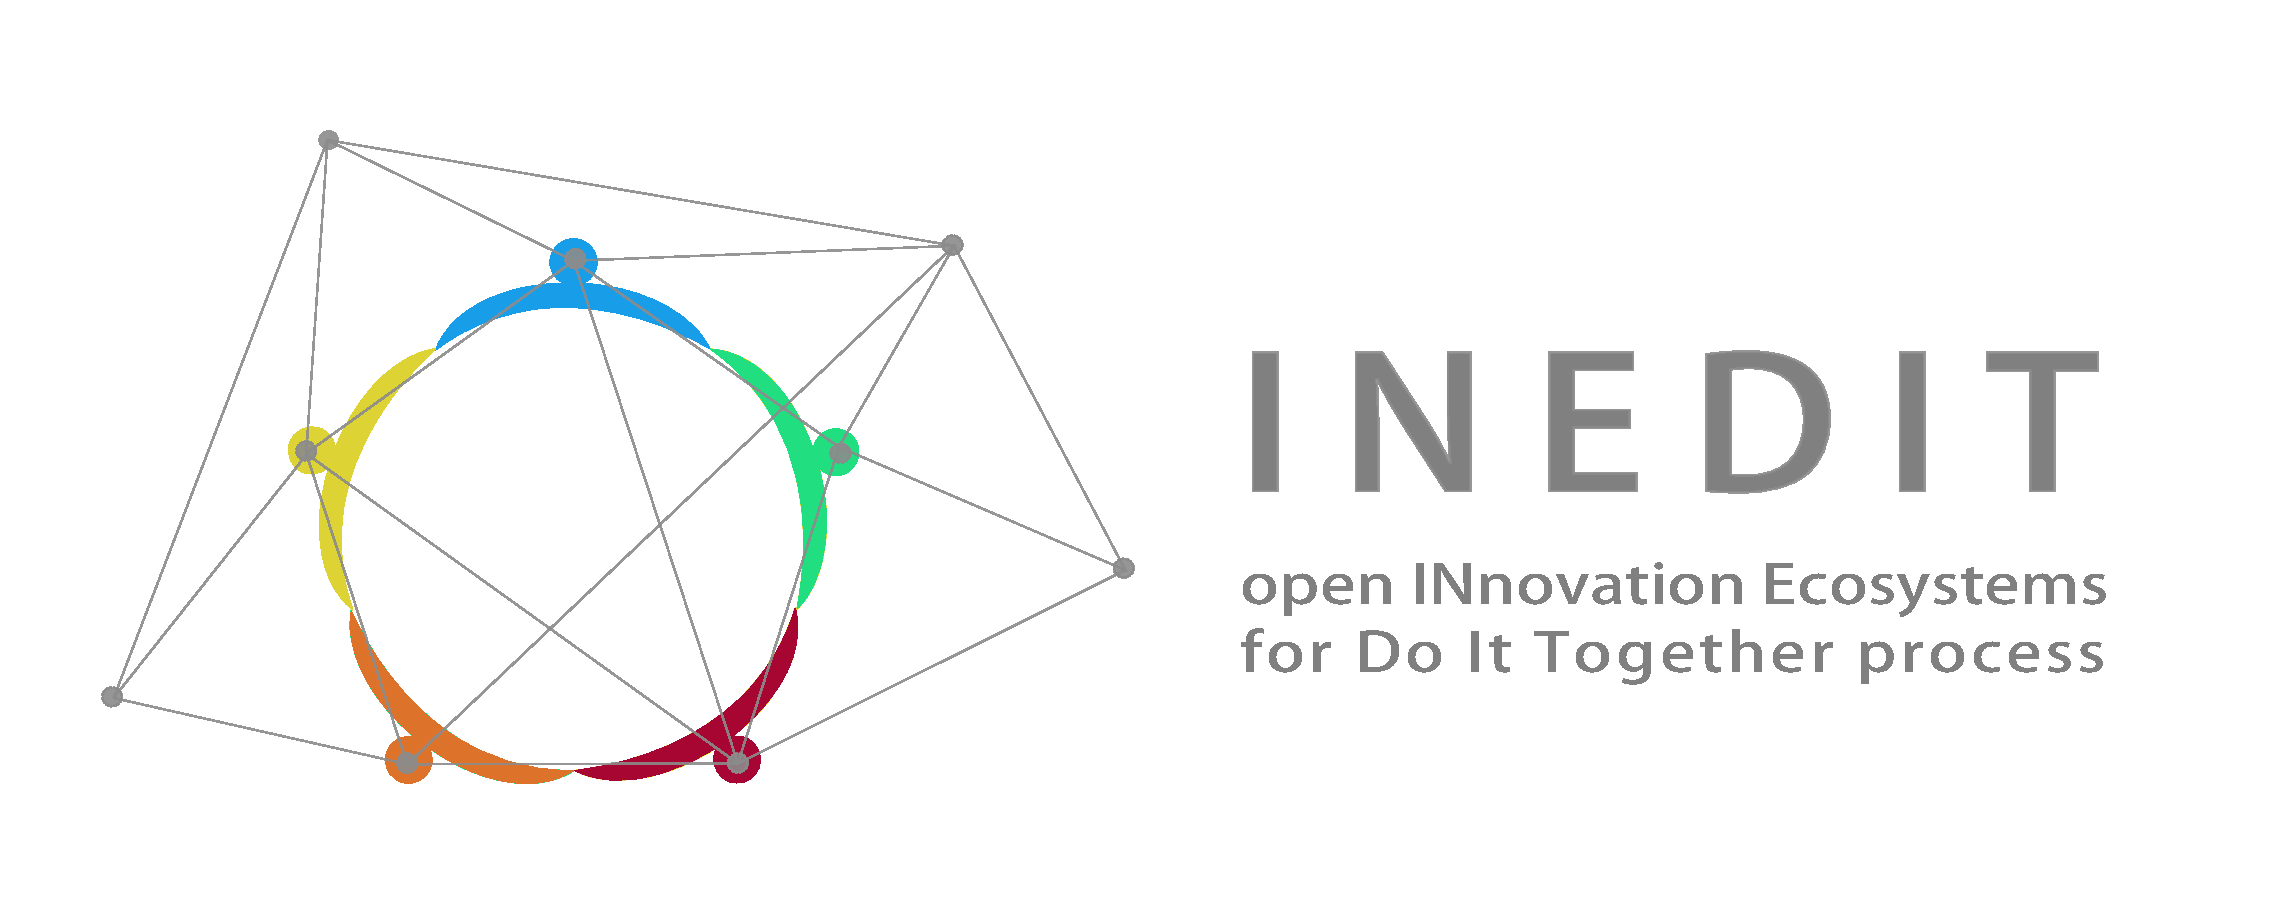
\includegraphics[width=\linewidth]{figures/Inedit_horiz.pdf}\\ 
		
		\vfill
		
		\textbf{\Huge{\textcolor{darkgray}{ D6.4 3D Printing of recycled plastic demonstrator }}} \\ 
		
		\vfill
		
		\vspace{60mm} 
		
		
		
      \textcolor{gray}{\rule{\textwidth}{2pt}}
      
		\vspace{5pt}
		\begin{tabular}{ c p{8cm} c }
           & & Version 1.0  \\ 
         WP6 T6.5  & & January 2023   \\ 
      \end{tabular}
		\vspace{5pt} 
		
		\textcolor{gray}{\rule{\textwidth}{2pt}}
		
		
	
		
		\vfill
		
	\end{center}
\end{titlepage}

\newpage


\begin{tabu} to \linewidth { X  X | X | X }
\toprule

 
\multicolumn{2}{l |}{ \multirow{4}{*}{  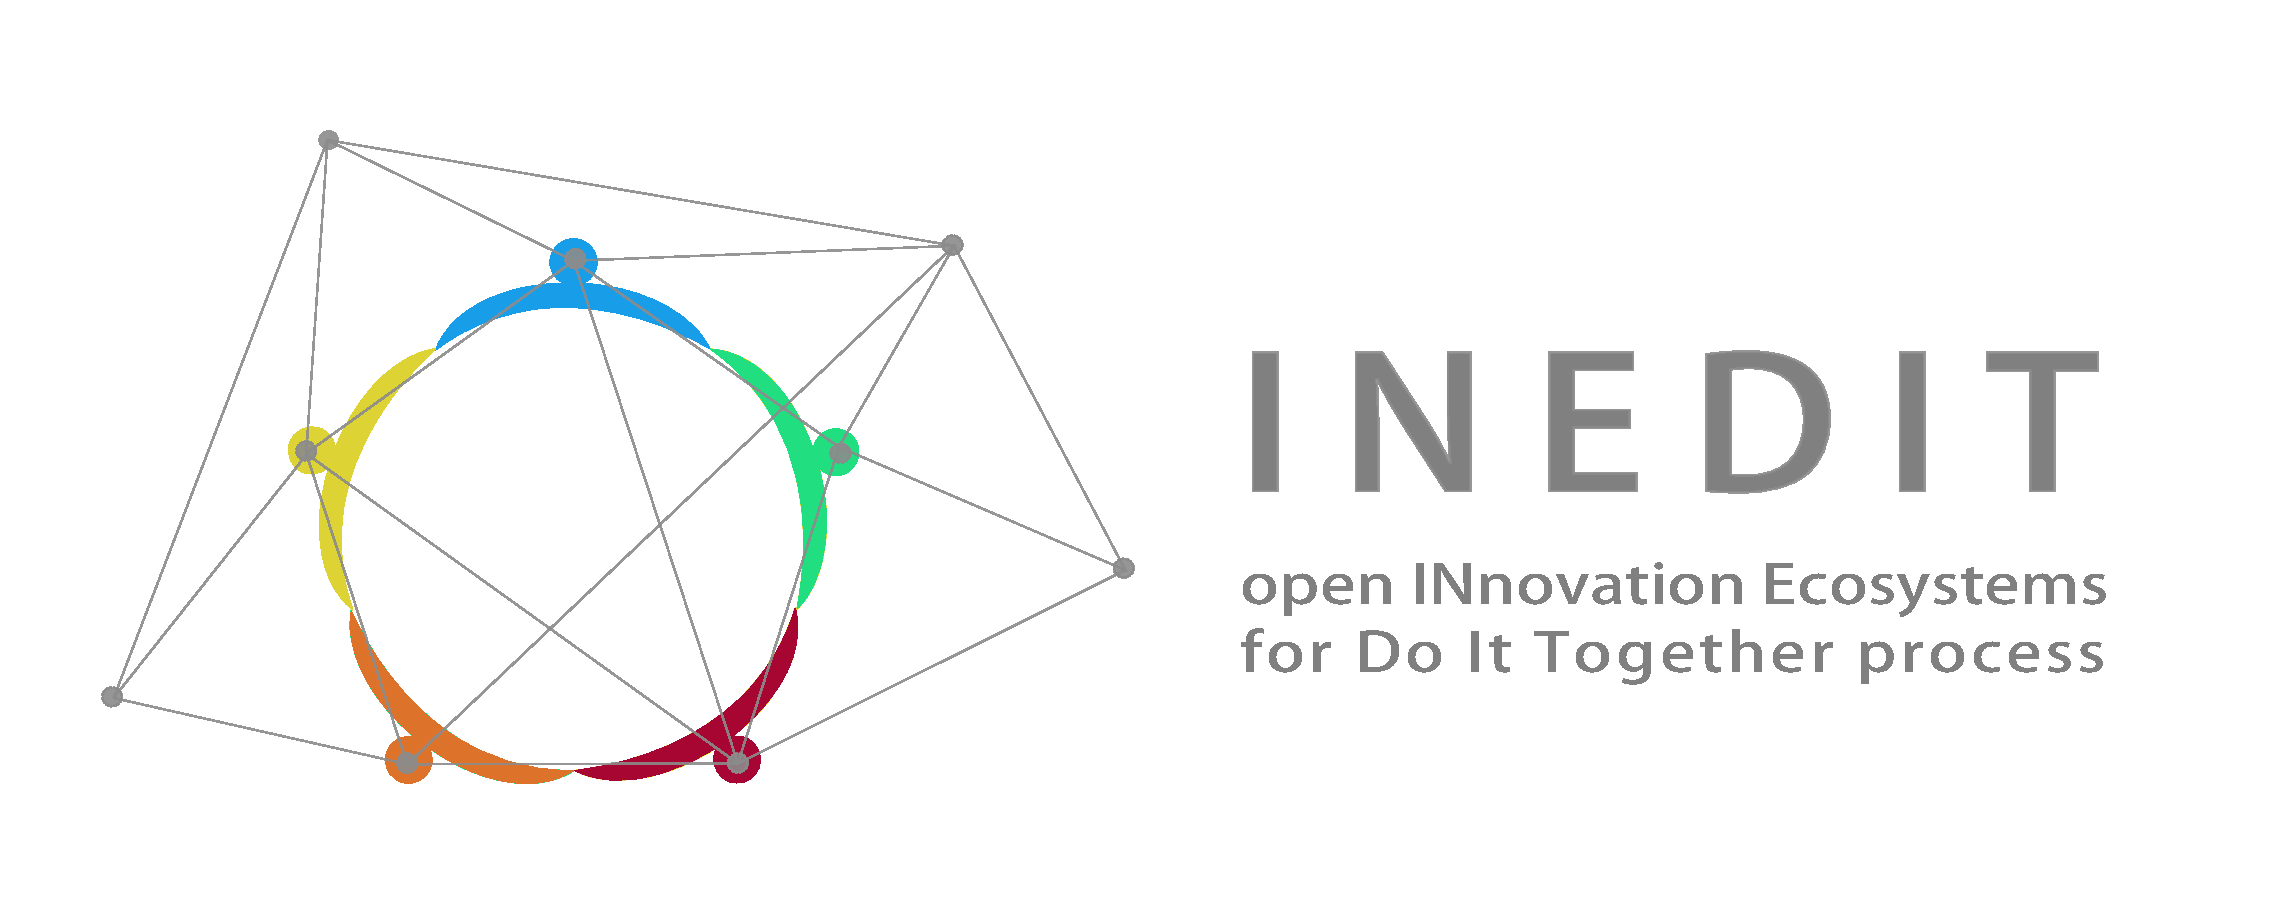
\includegraphics[width=7cm]{figures/Inedit_horiz.pdf} } }  & Work Package: & 6   \\ \cmidrule{3-4}
   & & Type of document:  & Deliverable        \\ \cmidrule{3-4}

   & & Due Delivery Date:    & January 31/2023     \\ \cmidrule{3-4}
 
   & & Actual Delivery Date:    & January 31 / 2023       \\ \midrule
 

\multicolumn{4}{l|}{ } \\ \midrule

 Responsible:    &  \multicolumn{3}{|l}{Université de Lorraine }        \\ \midrule
        
 Dissemination Level    &  \multicolumn{3}{|l}{ }  \\ \midrule
 Title:    &   \multicolumn{3}{|l}{ }    \\ \hline

 Description:    &    \multicolumn{3}{|l}{ }   \\ \midrule

 Version    &   \multicolumn{3}{|l}{ }    \\ \midrule
 Contributors       & Versions    & Dates       & Revision Description \\ \midrule
        
 & & & \\ \midrule
        
\end{tabu}


\vfill

\begin{center}
\textcolor{lightgray}{Disclaimer}

\textcolor{lightgray}{
\small
This document is provided « as is » with no warranties whatsoever, including any warranty or merchantability, non-infringement, fitness for any particular purpose, or any warranty otherwise arising out of any proposal, specification or sample.  No license, express or implied, by estoppels or otherwise, to any intellectual property rights are granted herein. The members of the project INEDIT do not accept any liability for actions or omissions of INEDIT members or third parties and disclaim any obligation to enforce the use of this document. }

\textcolor{lightgray}{
This document reflects only the authors' view and the Commission is not responsible for any use that may be made of the information it contains.  This document is subject to change without notice. 
}
\end{center}
\normalsize

\newpage

\ifdefined\Shaded\renewenvironment{Shaded}{\begin{tcolorbox}[frame hidden, borderline west={3pt}{0pt}{shadecolor}, sharp corners, enhanced, breakable, boxrule=0pt, interior hidden]}{\end{tcolorbox}}\fi

\renewcommand*\contentsname{Table of contents}
{
\hypersetup{linkcolor=}
\setcounter{tocdepth}{3}
\tableofcontents
}
\listoffigures
\color{darkgray}

\hypertarget{introduction}{%
\section{Introduction}\label{introduction}}

This deliverable deals with the description and implementation test of
the 3D printing of recycled plastic demonstrator. The ambition of this
use case is to test the feasibility of the distributed recycling via
additive manufacturing (DRAM)
(\protect\hyperlink{ref-CruzSanchez2020}{Cruz Sanchez et al., 2020})
concept with the purpose to integrate in the Do-It-Together approach.
There are two main goals:

Evaluate the technical and logistical feasibility of the distributed
recycling approach for the furniture sector, highlighting the advantages
and barriers found in the implementation process.

Provide a explain the a methodology in order

The document is structured in three main parts:

A baseline introduction is made regarding the plastic recycling issues
in order to

\hypertarget{plastic-issues-for-the-european-union}{%
\section{Plastic Issues for the European
Union}\label{plastic-issues-for-the-european-union}}

Since 1950', our society have gained enormous advantages in terms of
quality of life thanks to the technical development of the development
of plastic and polymer materials. Plastic is a material that is widely
used in our daily lives and plays a fundamental role in industry and
economic development. The plastic material are found in almost all our
products: food packaging, cars, technological tools, clothing, among
others. The main reason is that plastic materials offer a variety of
chemical and mechanical properties to be useful for a wide array of
applications. Plastics are extremely useful, but their mismanagement has
affected the environment and our health. The over-consumption and
especially bad practices (single use, difficulty of reuse, etc.), make
plastics one of the major societal challenges of an ecological
transition that has become imperative. The main problem is the
end-of-life treatment which traditionally uses a centralized system
where plastic waste often has to travel thousands of kilometers\ldots{}
to be incinerated or landfilled. In addition to the energy and
environmental impact of their production, there is also the impact of
the end of life.

Unfortunately, the plastic waste pollution poses a major threat because
of the issue of non-degradability affecting the ecological environments
(\protect\hyperlink{ref-Hopewell2009}{Hopewell et al., 2009};
\protect\hyperlink{ref-Ryberg2019}{Ryberg et al., 2019};
\protect\hyperlink{ref-Thompson2009b}{Thompson et al., 2009}). Indeed,
recycling rates remain small (approx. 14\%) in the plastic packaging
field on a global scale
(\protect\hyperlink{ref-Hahladakis2018}{Hahladakis and Iacovidou,
2018}). Even in Europe, which tends to lead on environmental
stewardship, the recycling rate is about 32.5 wt\%
(\protect\hyperlink{ref-Plastics2019}{Plastics, 2019}). However, these
values consider the amount of plastic waste collected, rather than the
total amount in circulation
(\protect\hyperlink{ref-Kranzinger2018}{Kranzinger et al., 2018}).
Rethinking the development and use of plastics is central to the
circular economy paradigm, to provide less harmful options for the
environment. Thus, more types of plastic packaging are available, but
each reflects diverse circular economy strategies

To tackle this accumulation waste problem, the European strategy for
plastics in the circular economy (CE) is gaining attention in the policy
and business debate surrounding sustainable development of industrial
production (\protect\hyperlink{ref-EC2018}{European Commission, 2018};
\protect\hyperlink{ref-Geissdoerfer2017}{Geissdoerfer et al., 2017}). CE
tackles a central societal issue concerning the current principle
``take, make, dispose'' (linear economy) and its negative effects caused
by the depletion of natural resources, waste generation, biodiversity
loss, pollution (water, air, soil) and non-sustainable economics
(\protect\hyperlink{ref-VanBuren2016}{van Buren et al., 2016}). The
validation (technical, economic, legislative) of waste plastic as a
secondary raw material in industrial processes is considered now a core
target to integrate CE into the plastic value chain
(\protect\hyperlink{ref-Simon2019}{Simon, 2019}). Strategies of open and
closed-loop recycling as well as upcycling and downcycling functionality
approaches can offer paths to validate the secondary raw materials
(\protect\hyperlink{ref-Zhuo2014}{Zhuo and Levendis, 2014}). The
promotion of cross-sectorial valorization of plastic wastes through
Industrial symbiosis approaches seems to be a relevant strategy for the
circular economy strategies of the EU
(\protect\hyperlink{ref-Karaylan2021}{Karayılan et al., 2021})

Based on this context, it is presented the demostration of the INEDIT
project called `3D Printing of Recycling Plastic' that was developed and
implemented. In the

\hypertarget{context-of-the-3d-printing-of-recycled-plastic-demostrator}{%
\section{Context of the 3D Printing of Recycled Plastic
Demostrator}\label{context-of-the-3d-printing-of-recycled-plastic-demostrator}}

\hypertarget{presentation-of-the-scale-of-the-demostrator-rives-de-meurthe-district-nancy-france}{%
\subsection{Presentation of the scale of the demostrator: Rives de
Meurthe district (Nancy,
France)}\label{presentation-of-the-scale-of-the-demostrator-rives-de-meurthe-district-nancy-france}}

The demonstrator is placed at the City of Nancy - France. Nancy is a
city located in northeastern France, in the region of Lorraine. It is
the capital of the Meurthe-et-Moselle department and has a population of
approximately 105,000 inhabitants.

It is the capital of the Meurthe-et-Moselle department, on the Meurthe
River in Lorraine. Nancy was the capital of the steel industry until its
collapse. In 1977, it created France's third largest technology park,
Nancy-Brabois, which is very accessible thanks to the highway network.

Located in the east of the city, the Rives de Meurthe district extends
from the banks of the Meurthe in the east to the boulevard Lobau and the
boulevard of the 26th infantry regiment in the west. To the south, it is
bounded by the rue de Tomblaine and to the north by the rue du Crosne.
It is separated from the rest of the city of Nancy by the canal from the
Marne to the Rhine. It thus gives the impression of being an independent
city, adjacent to Nancy.

\hypertarget{third-place-octroi-nancy}{%
\subsection{Third place Octroi Nancy}\label{third-place-octroi-nancy}}

The third place Octroi Nancy is a part of the neighborhood of the Rives
de Meurthe. This project transforms the former slaughterhouses of the
city of Nancy into \emph{``cultural, creative and citizen''} third place
with \(4600~m^2\) of renovated buildings
(\protect\hyperlink{ref-pallot2021}{Pallot et al., 2021}). Four large
buildings (Figure~\ref{fig-ok}) were adequated to provide a friendly and
multidisciplinary meeting place between culture and innovation; open to
experimentation and intended to operate as a creative laboratory for the
city. This place is intended to be an open space allowing the connection
of future occupants, such as artists and creatives, with the inhabitants
of the city and companies.

\begin{figure}

\begin{minipage}[t]{0.50\linewidth}

{\centering 

\raisebox{-\height}{


\includegraphics{figures/ok3/OK3.png}

}

}

\subcaption{\label{fig-oka}Description of the OK3 site}
\end{minipage}%
%
\begin{minipage}[t]{0.50\linewidth}

{\centering 

\raisebox{-\height}{


\includegraphics{figures/ok3/OK3.png}

}

}

\subcaption{\label{fig-okb}Photo of OK3}
\end{minipage}%

\caption{\label{fig-ok}The OK3 Site}

\end{figure}

At the 2023, this third place is an open ecosystem that will bring
together artists, researchers and creative people with the public, the
city's inhabitants and businesses.

\hypertarget{lorraine-fab-living-lab}{%
\subsection{\texorpdfstring{Lorraine Fab Living
Lab\textregistered}{Lorraine Fab Living Lab}}\label{lorraine-fab-living-lab}}

The \textbf{Lorraine Smart Cities Living Lab (LSCLL)} is a
trans-disciplinary resource center of the Université de Lorraine, to
support and link the different societal challenges of the Lorraine
territory with the local resources. It enables the integration of
different users, implementing collaborative and agile approaches in the
service of \emph{Research, Development of Innovations, Training and a
Citizen Culture}. It experiments in terms of projects, governance and
support platform since 2008, involving several laboratories and other
public and private partners as detailed in the Figure~\ref{fig-LSCLL}.
Since 2010, this project is member of the European Network of Living
Labs (ENoLL)\footnote{\(4^{th}\) wave of labelisation)}, seeking to
develop public-private-population Partnerships (PPPPs) to disseminate
innovation and related practices.

\begin{figure}

\begin{minipage}[t]{0.50\linewidth}

{\centering 

\raisebox{-\height}{

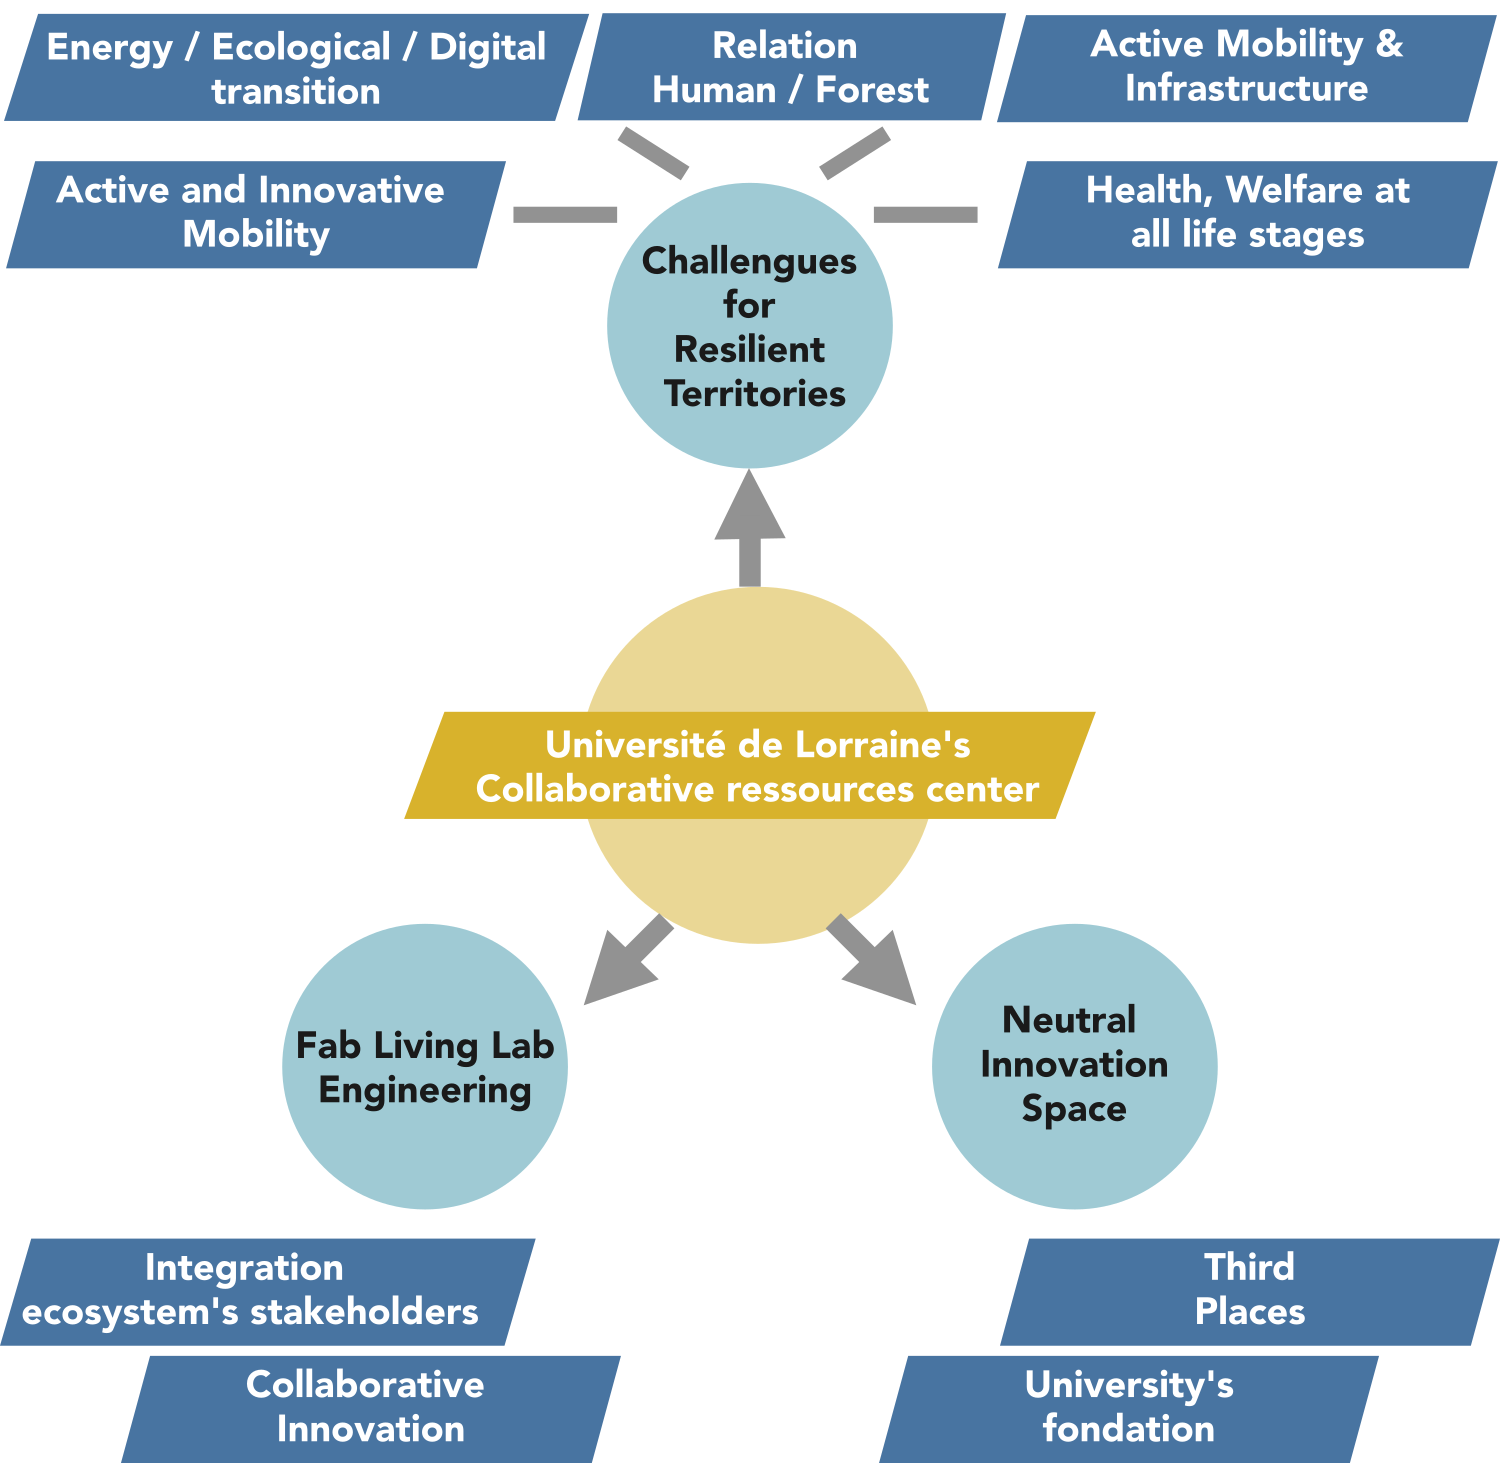
\includegraphics{figures/lf2l/LSCLL.png}

}

}

\subcaption{\label{fig-LSCLL}Description of the Lo site}
\end{minipage}%
%
\begin{minipage}[t]{0.50\linewidth}

{\centering 

\raisebox{-\height}{


\includegraphics{figures/ok3/OK3.png}

}

}

\subcaption{\label{fig-okb}Photo of OK3}
\end{minipage}%

\caption{\label{fig-lscll}The OK3 Site}

\end{figure}

Since 2014, the LSCLL formalizes its strategic intention with the the
Lorraine Fab Living Lab\textregistered    (LF2L\textregistered) research
platform for prospective assessment of innovative usages
(\protect\hyperlink{ref-Dupont2016}{Dupont et al., 2016}).\\
The LF2L physical environment is constituted by a collaborative and a
fabLab space. The collaborative space allows users to foster
co-operation in engineering design with different stakeholders in order
to new create concepts/designs. On the other hand, FabLab space allows
users to materialize the concepts/designs in an easy and quick way in
order to have an prospective evaluation
(\protect\hyperlink{ref-Boujut2003}{Boujut and Blanco, 2003};
\protect\hyperlink{ref-Dupont2015b}{Dupont et al., 2015},
\protect\hyperlink{ref-Dupont2014}{2014}). The synergy of these two
spaces enables the project development in a living lab approach taking
into account the User Centered Design principles.

The conceptual framework is composed of three main elements as
illustrated in Figure~\ref{fig-lf2l-methodology}:

\begin{figure}

\begin{minipage}[t]{0.50\linewidth}

{\centering 

\raisebox{-\height}{

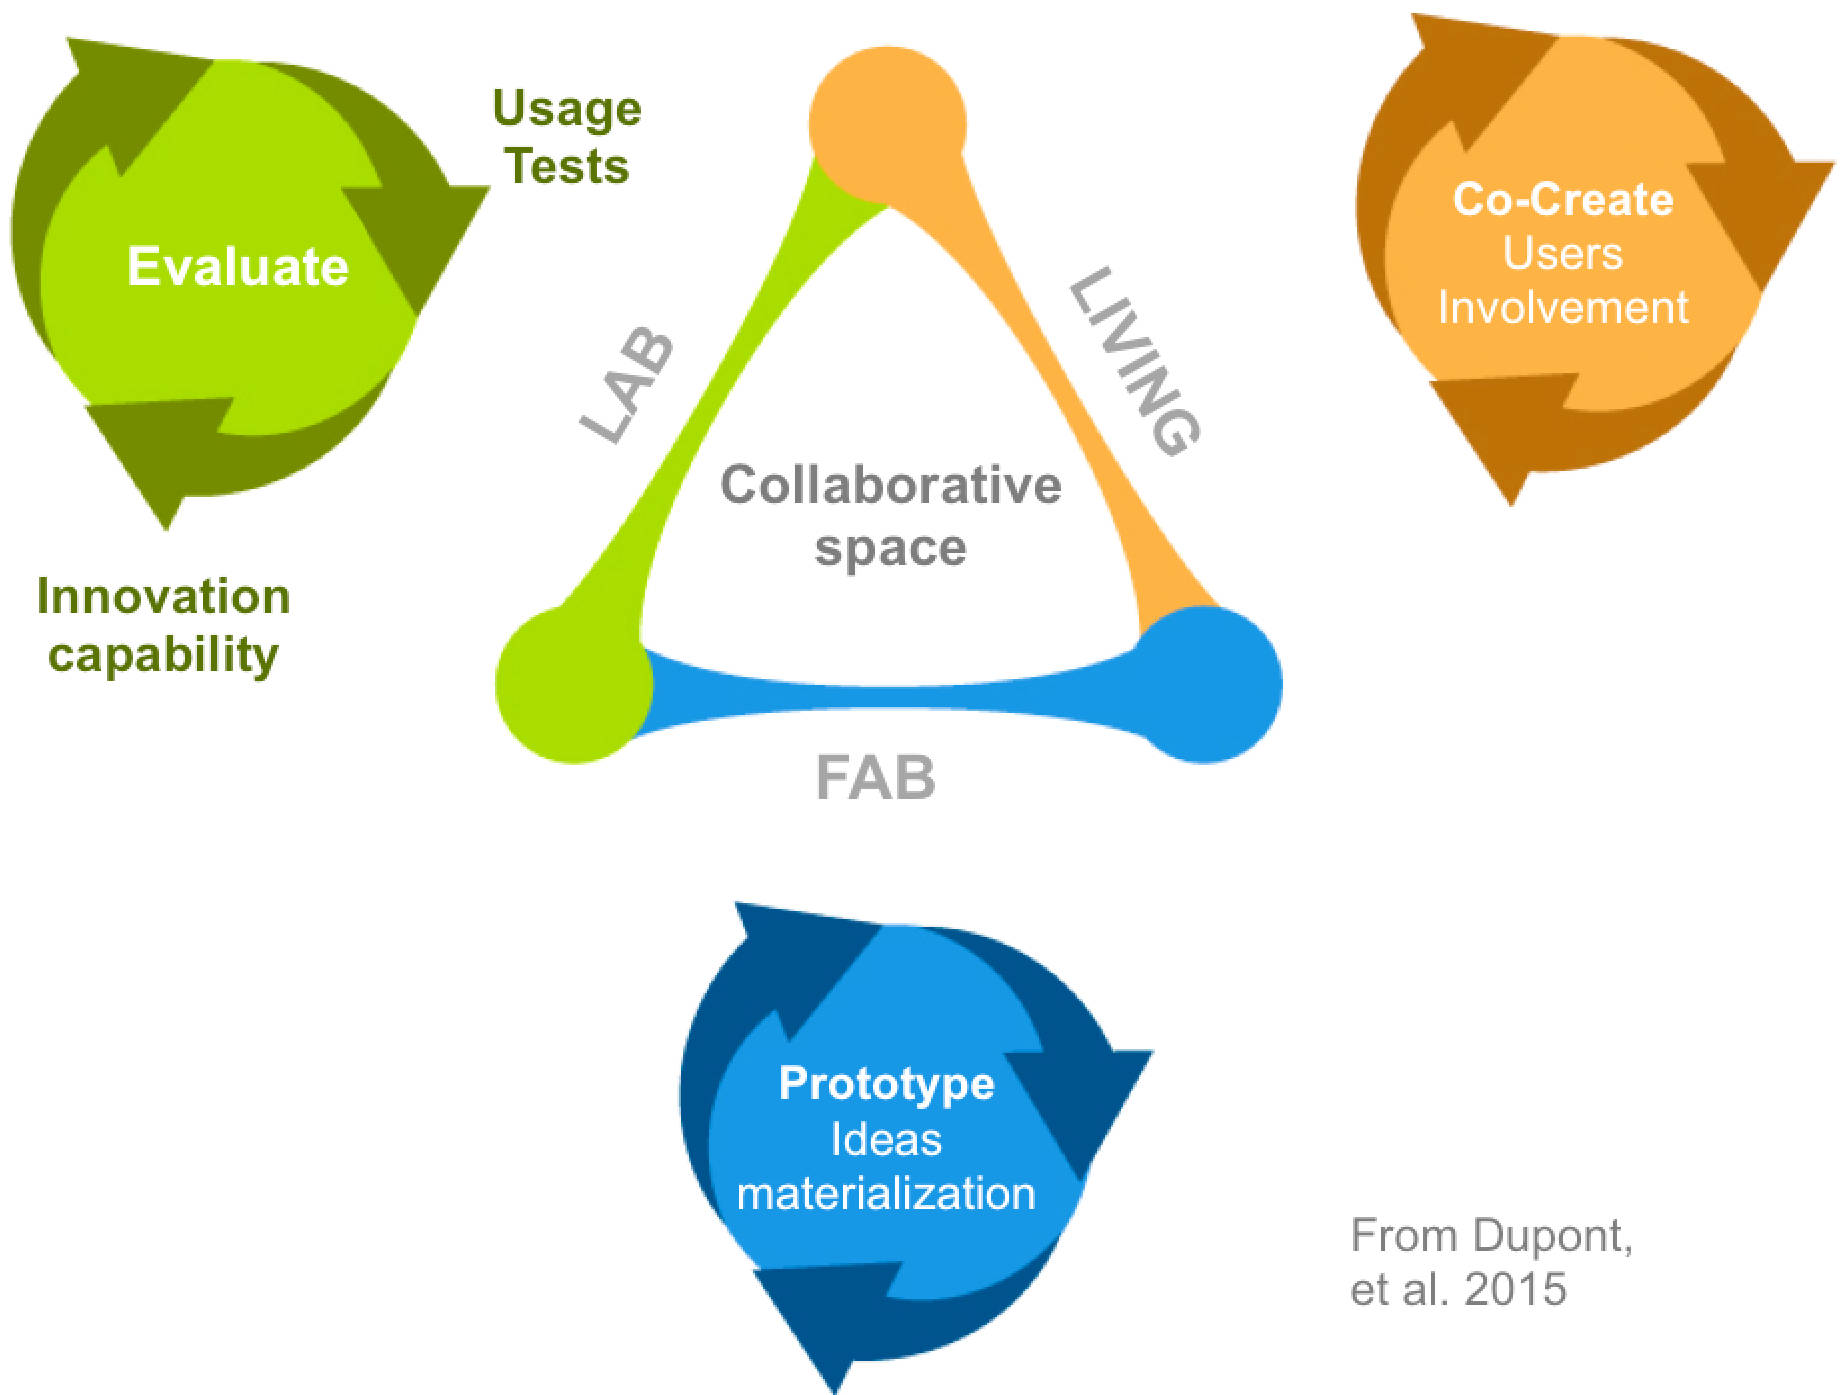
\includegraphics{figures/lf2l/Methodology-01.jpg}

}

\caption{\label{fig-lf2l-methodology}The Lorraine Fab Living Lab
methodlogy.}

}

\end{minipage}%
%
\begin{minipage}[t]{0.50\linewidth}

{\centering 

\begin{enumerate}
\def\labelenumi{\arabic{enumi}.}
\tightlist
\item
  \emph{Co-creation}: Creative process to find alternative resolution
  concepts to a problem-topic given integrating the key stakeholders in
  the process.
\item
  \emph{Prototyping}: Materialization (virtual/real) of the concept in
  order to have a first and quick in- sight.
\item
  \emph{Evaluation}: Establishment of the pertinence of the concepts in
  order to create a feedback/improvement process.
\end{enumerate}

}

\end{minipage}%

\end{figure}

The conceptual innovation framework of LF2L takes into consideration the
2D (concept), 3D (object), 4D (over time) approaches involving different
type of stakeholders (e.g.~researches, companies, networks,) in order to
have a foresight usage evaluation of a new concept, technology or
project. The stages and 2D/3D/4D resources allowing prospective
assessment of innovative usages in order to support this conceptual
framework inside this ``innovation space'' as indicated in figure 2.3
(\protect\hyperlink{ref-Dupont2016}{Dupont et al., 2016},
\protect\hyperlink{ref-Dupont2015b}{2015}): This approach is useful to
accelerate the deployment of industrial and/or urban demonstrators.

\hypertarget{d-printing-of-recycled-plastic-demonstrator-the-green-fablab}{%
\section{3D Printing of recycled plastic demonstrator: the ``Green
FabLab''}\label{d-printing-of-recycled-plastic-demonstrator-the-green-fablab}}

\hypertarget{rationale-for-the-technological-system-of-the-3d-printing-recycling-demonstrator}{%
\subsection{Rationale for the technological system of the 3D printing
recycling
demonstrator}\label{rationale-for-the-technological-system-of-the-3d-printing-recycling-demonstrator}}

Based on the context characteristics of the (LF2L\textregistered) and
the Octroi local ecosystems, the 3D printed demonstrator, also called
locally as the \emph{``Green Fablab''} as illustrated in the
Figure~\ref{fig-gf-2021}, it is an initial socio-technical demonstrator
of the distributed recycling approach that combines a living lab
approach inside a citizen third place ecosystem.

\begin{figure}[H]

{\centering 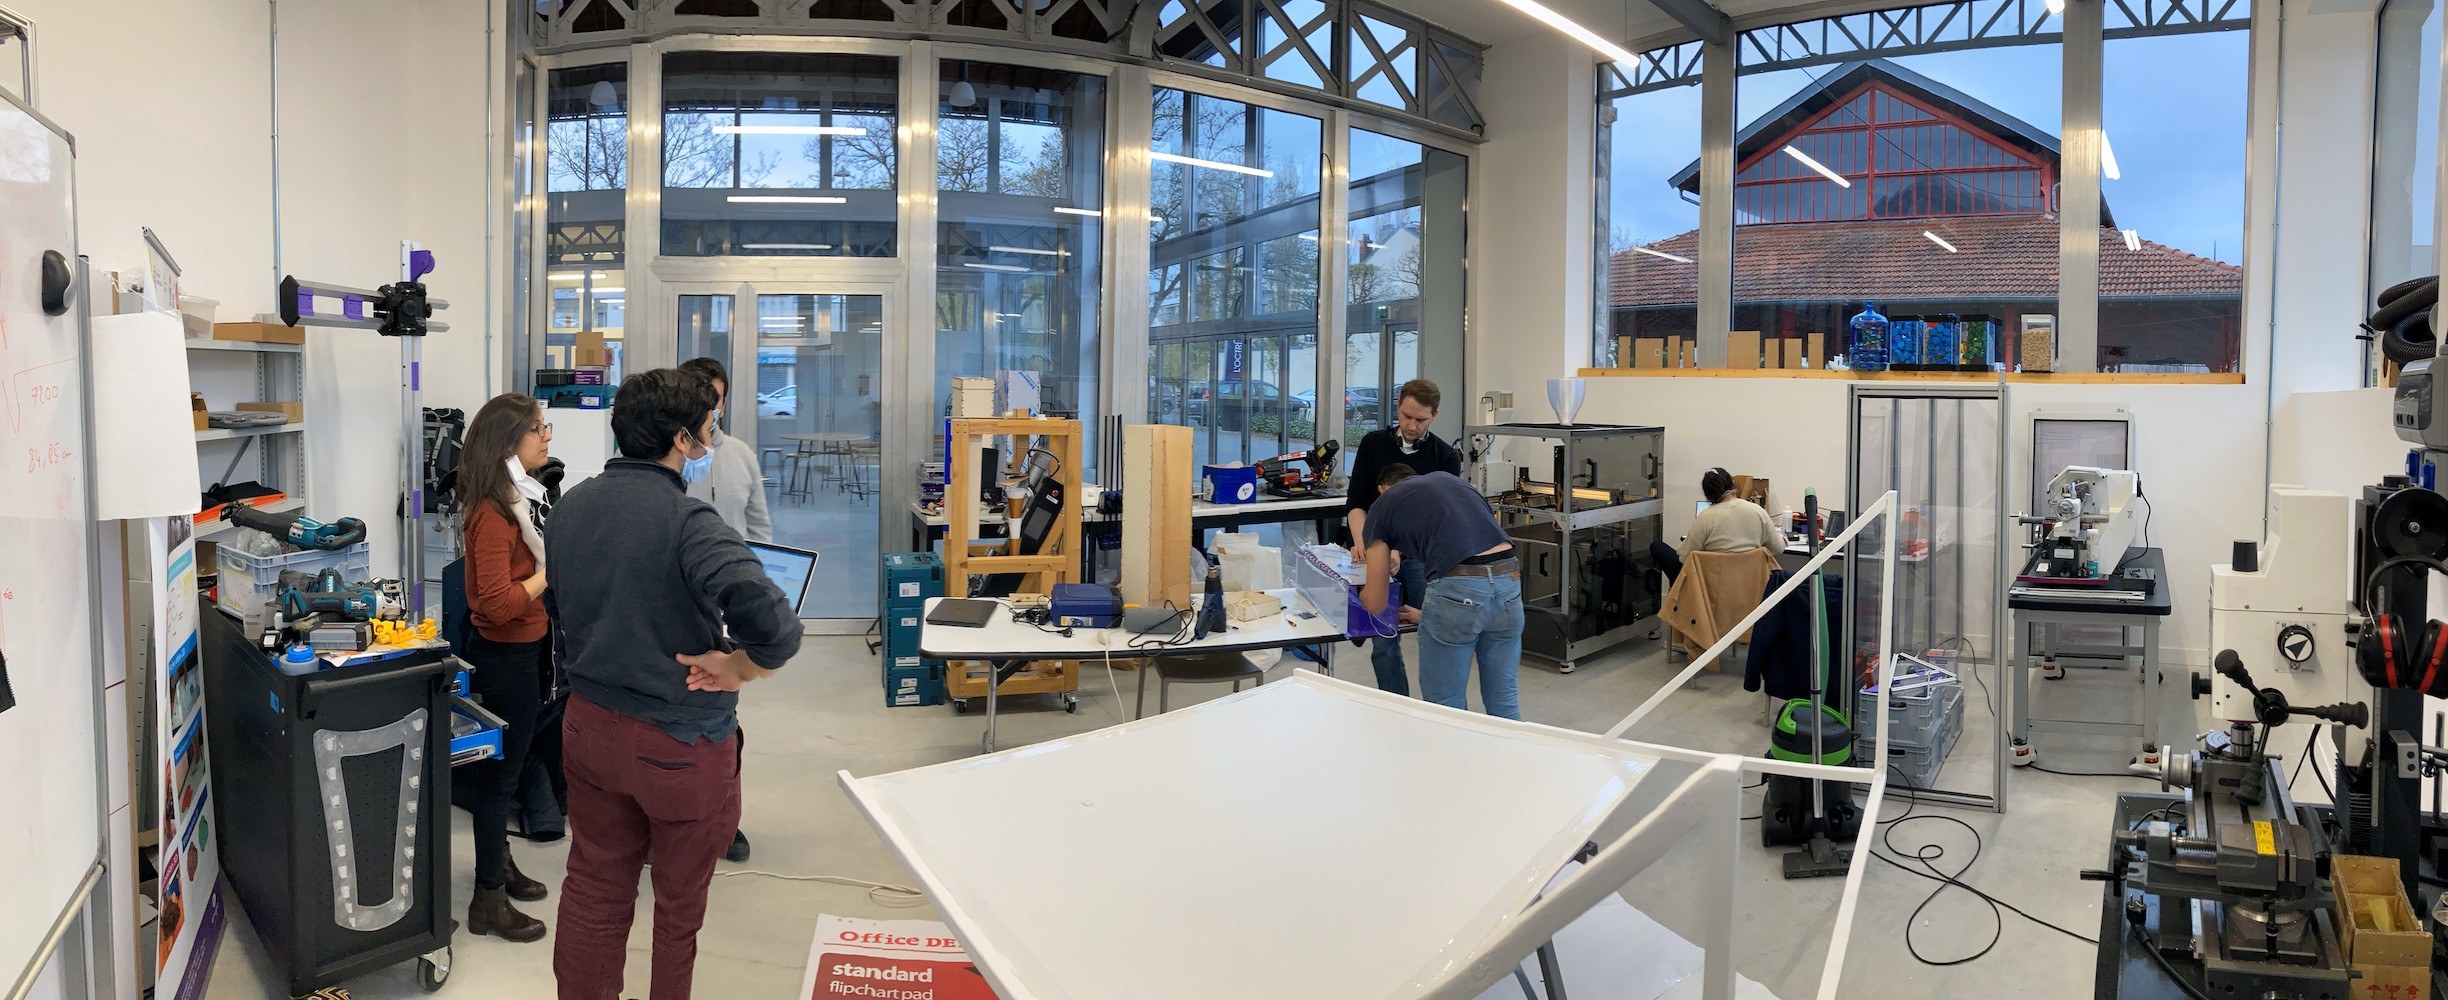
\includegraphics[width=0.9\textwidth,height=\textheight]{figures/2021-11-17-octroi.jpeg}

}

\caption{\label{fig-gf-2021}Initial overview of the Green Fablab at
November 2021}

\end{figure}

The Green FabLab demonstrator aims to experiment the technical
feasibility and evaluation of a distributed and local plastic recycling.
The main purpose is to valorize plastic waste for 3D printing technology
and manual injection moulding techniques in the context of an open
innovation space such as the Octroi Nancy. The results of this
experimentation can be a baseline for many archetypes of open
communities such as fab labs, Hackerspaces or even industrial
prototyping zones.

The main purpose of this demonstrator in the INEDIT project is
\textbf{to prove that plastic waste material can have several uses, and
therefore several values, during its life cycle}. The same material
could be recycled and transformed into new raw material for different
products. It is in this spirit that many associations, SMEs, local
authorities and individuals are developing new local recycling practices
that could allow us to aim for an economy that is more respectful of the
environment, fairer for society and more engaging for local politicians.

Therefore, it is neccesary to understand the key conditions under which
to deploy a notion of circular economy with plastic waste to possible
establish a secondary raw material market for this asset. Likewise, it
is required the study of technical parameters for the technological
diversity to possible use the waste material including the open source
3D printers and manual desktop injection. The outputs are, not only by
minimizing use of the environment as a sink for residuals but -- perhaps
more importantly -- by minimizing the use of virgin materials. Hence,
the environmental impact of this technology is significantly reduced.

Moreover, taking into account the exponential growth of these spaces
(Fablab, Hakerspace, Makespace), they could help to increase the
efficiency to the problem of polymer recycling through the development
of a distributed recycling approach. In these geographically distributed
spaces, the polymer recycling process of the surrounding areas (streets,
neighbourhood, industrial zones) will be carried out at small lot sizes
minimizing, energy consumptions, and carbon emissions compared to the
tradition centralized systems, as some researches have already explored
this path.

\hypertarget{distributed-recycling-via-additive-manufacturing-dram}{%
\subsection{Distributed recycling via Additive Manufacturing
DRAM}\label{distributed-recycling-via-additive-manufacturing-dram}}

The Additive manufacturing (AM) -also known as 3D printing- is an
important industrial vector in the and its direct (and distributed)
manufacturing capabilities is becoming a key industrial process that
could play a relevant role in the transition from a linear to circular
economy (\protect\hyperlink{ref-Despeisse2016}{Despeisse et al., 2017}).
AM technologies is expected to transform the production process
(\protect\hyperlink{ref-Chen2017}{Chen et al., 2017};
\protect\hyperlink{ref-Jiang2017}{Jiang et al., 2017};
\protect\hyperlink{ref-Rahman2018}{Rahman et al., 2018}) thanks to its
ability to transform a numerical model into a deposition of material
(points, lines or areas) to create a 3D part
(\protect\hyperlink{ref-Bourell2017}{Bourell et al., 2017}). The
expiration of the first patents has contributed to an increased
interest, creating consumer value and potential for disruption
(\protect\hyperlink{ref-Beltagui2020}{Beltagui et al., 2021};
\protect\hyperlink{ref-West2016a}{West and Kuk, 2016}). In economic
terms, the global additive manufacturing market is expected to reach USD
23.33 billion by 2026 (\protect\hyperlink{ref-ReportsAndData2019}{Data,
2019}). However, determining when and how to take advantage of the
benefits is a challenge for traditional means of production. From a
societal viewpoint, Jiang et al.
(\protect\hyperlink{ref-Jiang2017}{2017}) reported that the product
development could change from traditional stage-gate models to
iterative, agile processes changing the scenario by 2030.

The technical development of INEDIT's demonstrator is based on the
\textbf{distributed recycling via additive manufacturing (DRAM) approach
(\protect\hyperlink{ref-CruzSanchez2020}{Cruz Sanchez et al., 2020}).
This approach is a major scientific output from the INEDIT project as a
proposition of the future industrial landscape}.

DRAM is defined as the use of recycled materials by means of mechanical
recycling process in the 3D printing process chain. In the literature,
DRAM approach emphasizes the technical steps required to reuse plastic
waste through the recycling chains for material-extrusion-based 3D
printing (\protect\hyperlink{ref-CruzSanchez2020}{Cruz Sanchez et al.,
2020}; \protect\hyperlink{ref-Little2020}{Little et al., 2020}). The use
of recycled material, either in the form of raw material or blended with
virgin material, is a method of special interest to contribute to
sustainable manufacturing (\protect\hyperlink{ref-Zhao2018}{Zhao et al.,
2018}).

Figure~\ref{fig-dram} illustrates the conceptual model of DRAM.

\begin{figure}[H]

{\centering 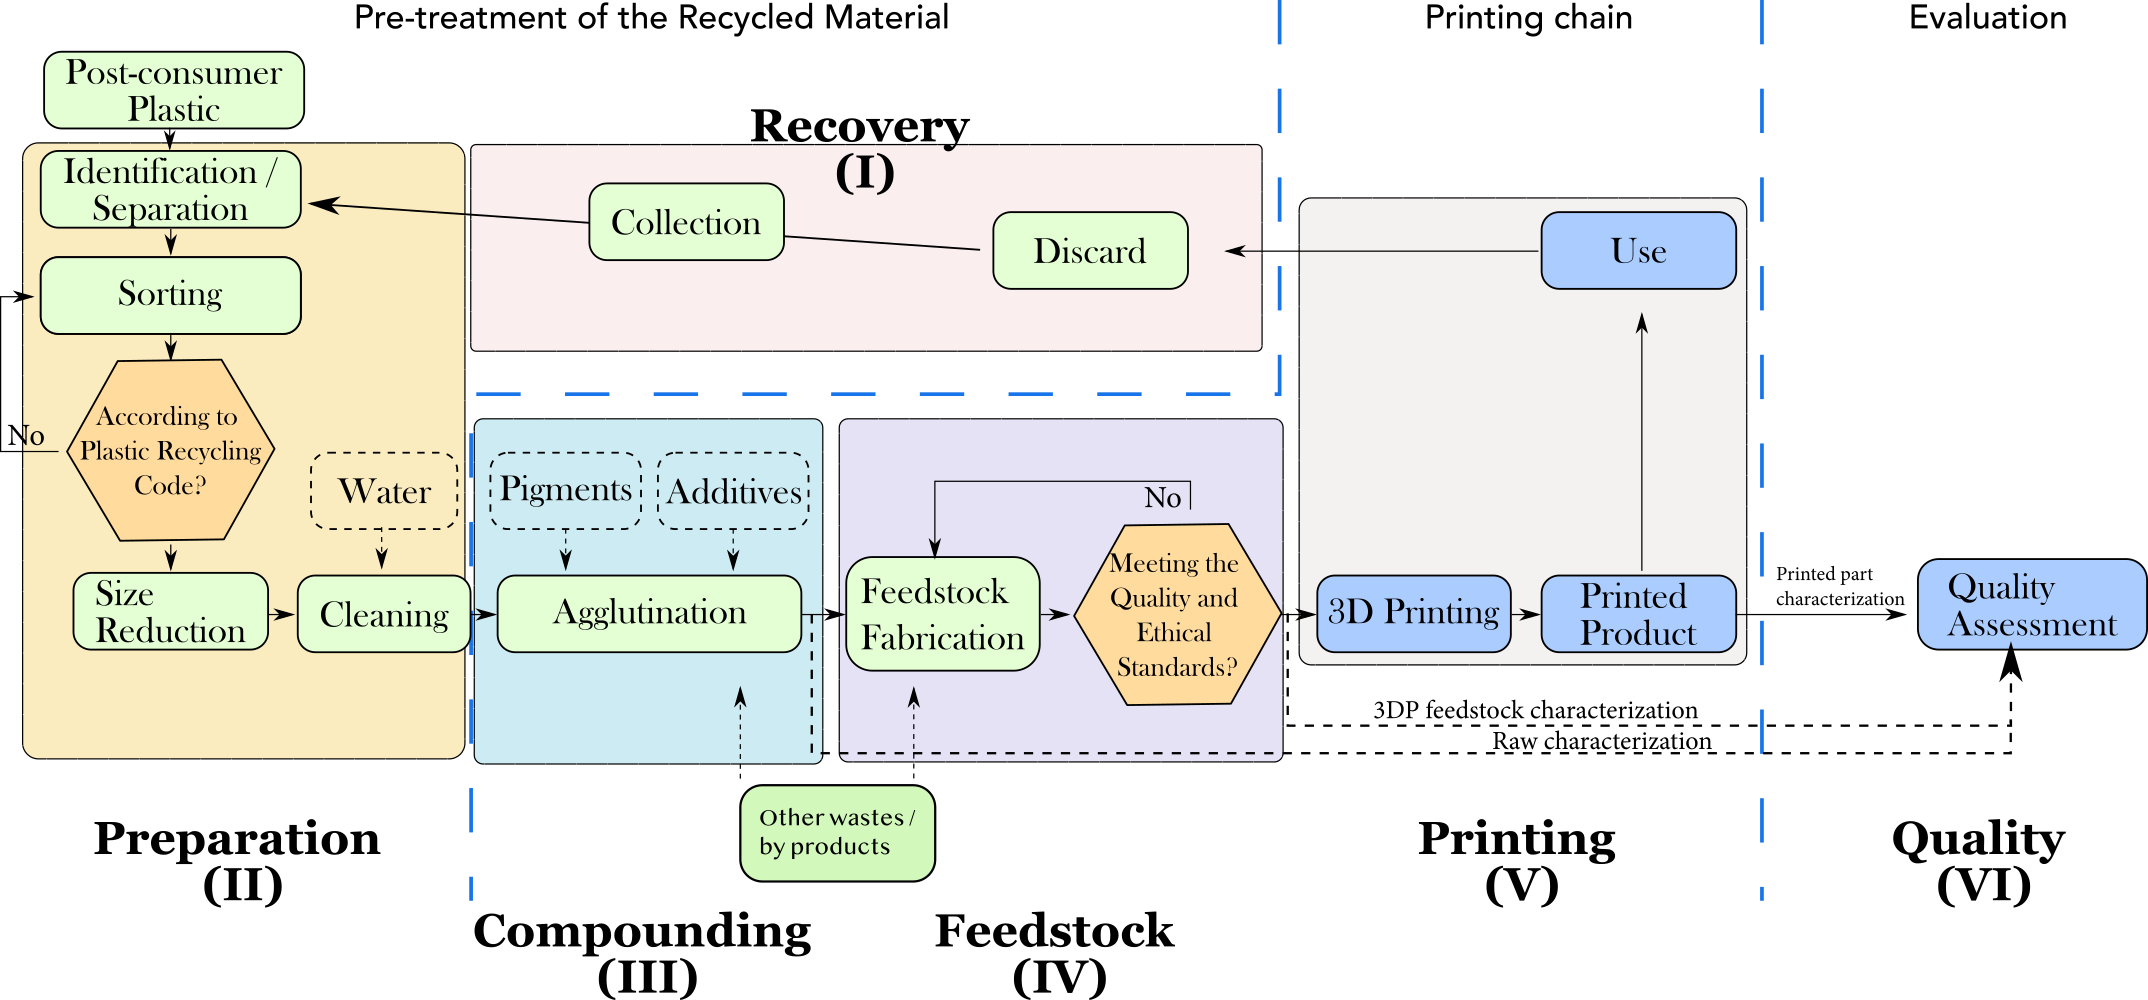
\includegraphics[width=0.9\textwidth,height=\textheight]{figures/DRAM-10.png}

}

\caption{\label{fig-dram}DRAM}

\end{figure}

In a general overview, the \textbf{Recovery (I)} phase concerns the
logistic operations to consider to collect the plastic wastes to be
reused in DRAM. The \textbf{Preparation (II)} phase corresponds to the
actions and strategies to identify, separate, sort, size reduce and
clean waste plastic to guarantee adequate quality for DRAM. The
\textbf{Compounding (III)} phase refers to the development of mono- and
composite-materials. The \textbf{Feedstock (IV)} phase identifies the
actions to fabricate the material usable for the printing process,
either filament for Fused Filament Fabrication (FFF) or the particle
size for Fused Granular Fabrication (FGF). The \textbf{Printing (V)}
stage identifies applications and process improvements for the recycled
printed part. The \textbf{Quality (VI)} phase identifies the multi-level
technical characterization performed to the recycled material.

In the DRAM methodology, consumers have an economic incentive to
recycle. This is because they can use their waste as feedstock for a
wide range of consumer products that can be produced for a fraction of
the conventional cost of the equivalent products. Moreover, 3D printing
is especially well suited because it enables the production of parts
with (almost) no waste, and could reduce the waste related to the
material by more than 40 \%, reusing 95\% of the unused material
(\protect\hyperlink{ref-Petrovic2011}{Petrovic et al., 2011}).\\
Currently, most of the cost of 3D printing is associated with filament
(\protect\hyperlink{ref-Wittbrodt2013}{Wittbrodt et al., 2013}). By
recycling raw materials such as Polylactic acid (PLA), one of the most
frequently used materials in 3D printing, it is possible to reduce the
carbon dioxide emissions that are incurred by transport to landfills or
shipping to customers, offering environmental benefits
(\protect\hyperlink{ref-Santander2020}{Santander et al., 2020}).

A large number of products can already be manufactured with AM, which
affects the geographical spread and density of global value chains
(\protect\hyperlink{ref-Laplume2016}{Laplume et al., 2016}). It is
expected that the reach of AM printable products will be much greater in
the future, as the production of multi-material and built-in
functionalities (e.g.~electronics) will be possible to a large extent.
In addition, the production of spare parts can be carried out on-site,
modifying the role of suppliers in the production lines
(\protect\hyperlink{ref-Zanoni2019}{Zanoni et al., 2019}). Matt et al.
(\protect\hyperlink{ref-Matt2015}{2015}) explored the stages of
distributed model factories and decentralized production types ranging
from distributed capabilities to cloud production. Thus, the need of
transport will be much more carefully because the fact that AM will
enable decentralization of production to localities near customers or in
the most extreme distributed scenario at the customer's premises
(\protect\hyperlink{ref-BonninRoca2019}{Bonnín Roca et al., 2019};
\protect\hyperlink{ref-Petersen2017a}{Petersen and Pearce, 2017};
\protect\hyperlink{ref-Wittbrodt2013}{Wittbrodt et al., 2013}).
Moreover, AM technology makes it possible to reduce market entry
barriers, reduce capital requirements and achieve an efficient minimum
scale of production to promote distributed, flexible forms of production
(\protect\hyperlink{ref-Despeisse2016}{Despeisse et al., 2017}).

The distributed manufacturing/recycling approach enables an alternative
option from an economy-of-scale to an economy-of-scope, where the
products are highly personalized satisfying niche communities or even
individuals (\protect\hyperlink{ref-Hienerth2014}{Hienerth et al.,
2014}; \protect\hyperlink{ref-Petrick2014}{\textbf{Petrick2014?}}). For
these reasons, the AM technology could be a driver for a shift in
manufacturing from globally distributed production to local facilities.
Significant efforts are being made by industry and the scientific
community to move AM techniques from rapid prototyping and tooling
stages towards direct digital manufacturing (DDM)
(\protect\hyperlink{ref-Mueller2012}{Gibson et al., 2010};
\protect\hyperlink{ref-Holmstrom2016}{Holmström et al., 2016}), with the
concomitant environmental and social benefits. Nevertheless, Niaki et
al. (\protect\hyperlink{ref-Niaki2019}{2019}) demonstrated that
environmental and social benefits are not the key preferential factors
in the adoption of AM technologies in different industrial sectors. Only
the economic factor remains relevant in the AM implementation,
considering time- and cost-saving as the most important reasons.

\hypertarget{positionnement-of-use-case-for-omdf-functions}{%
\subsection{Positionnement of Use case for OMDF
Functions}\label{positionnement-of-use-case-for-omdf-functions}}

Considering the Open Manufacturig Demonstrateion Facilities functions
established in the Delivrable XX.X, the Green fablab proves the
following functions:

\begin{figure}[H]

{\centering 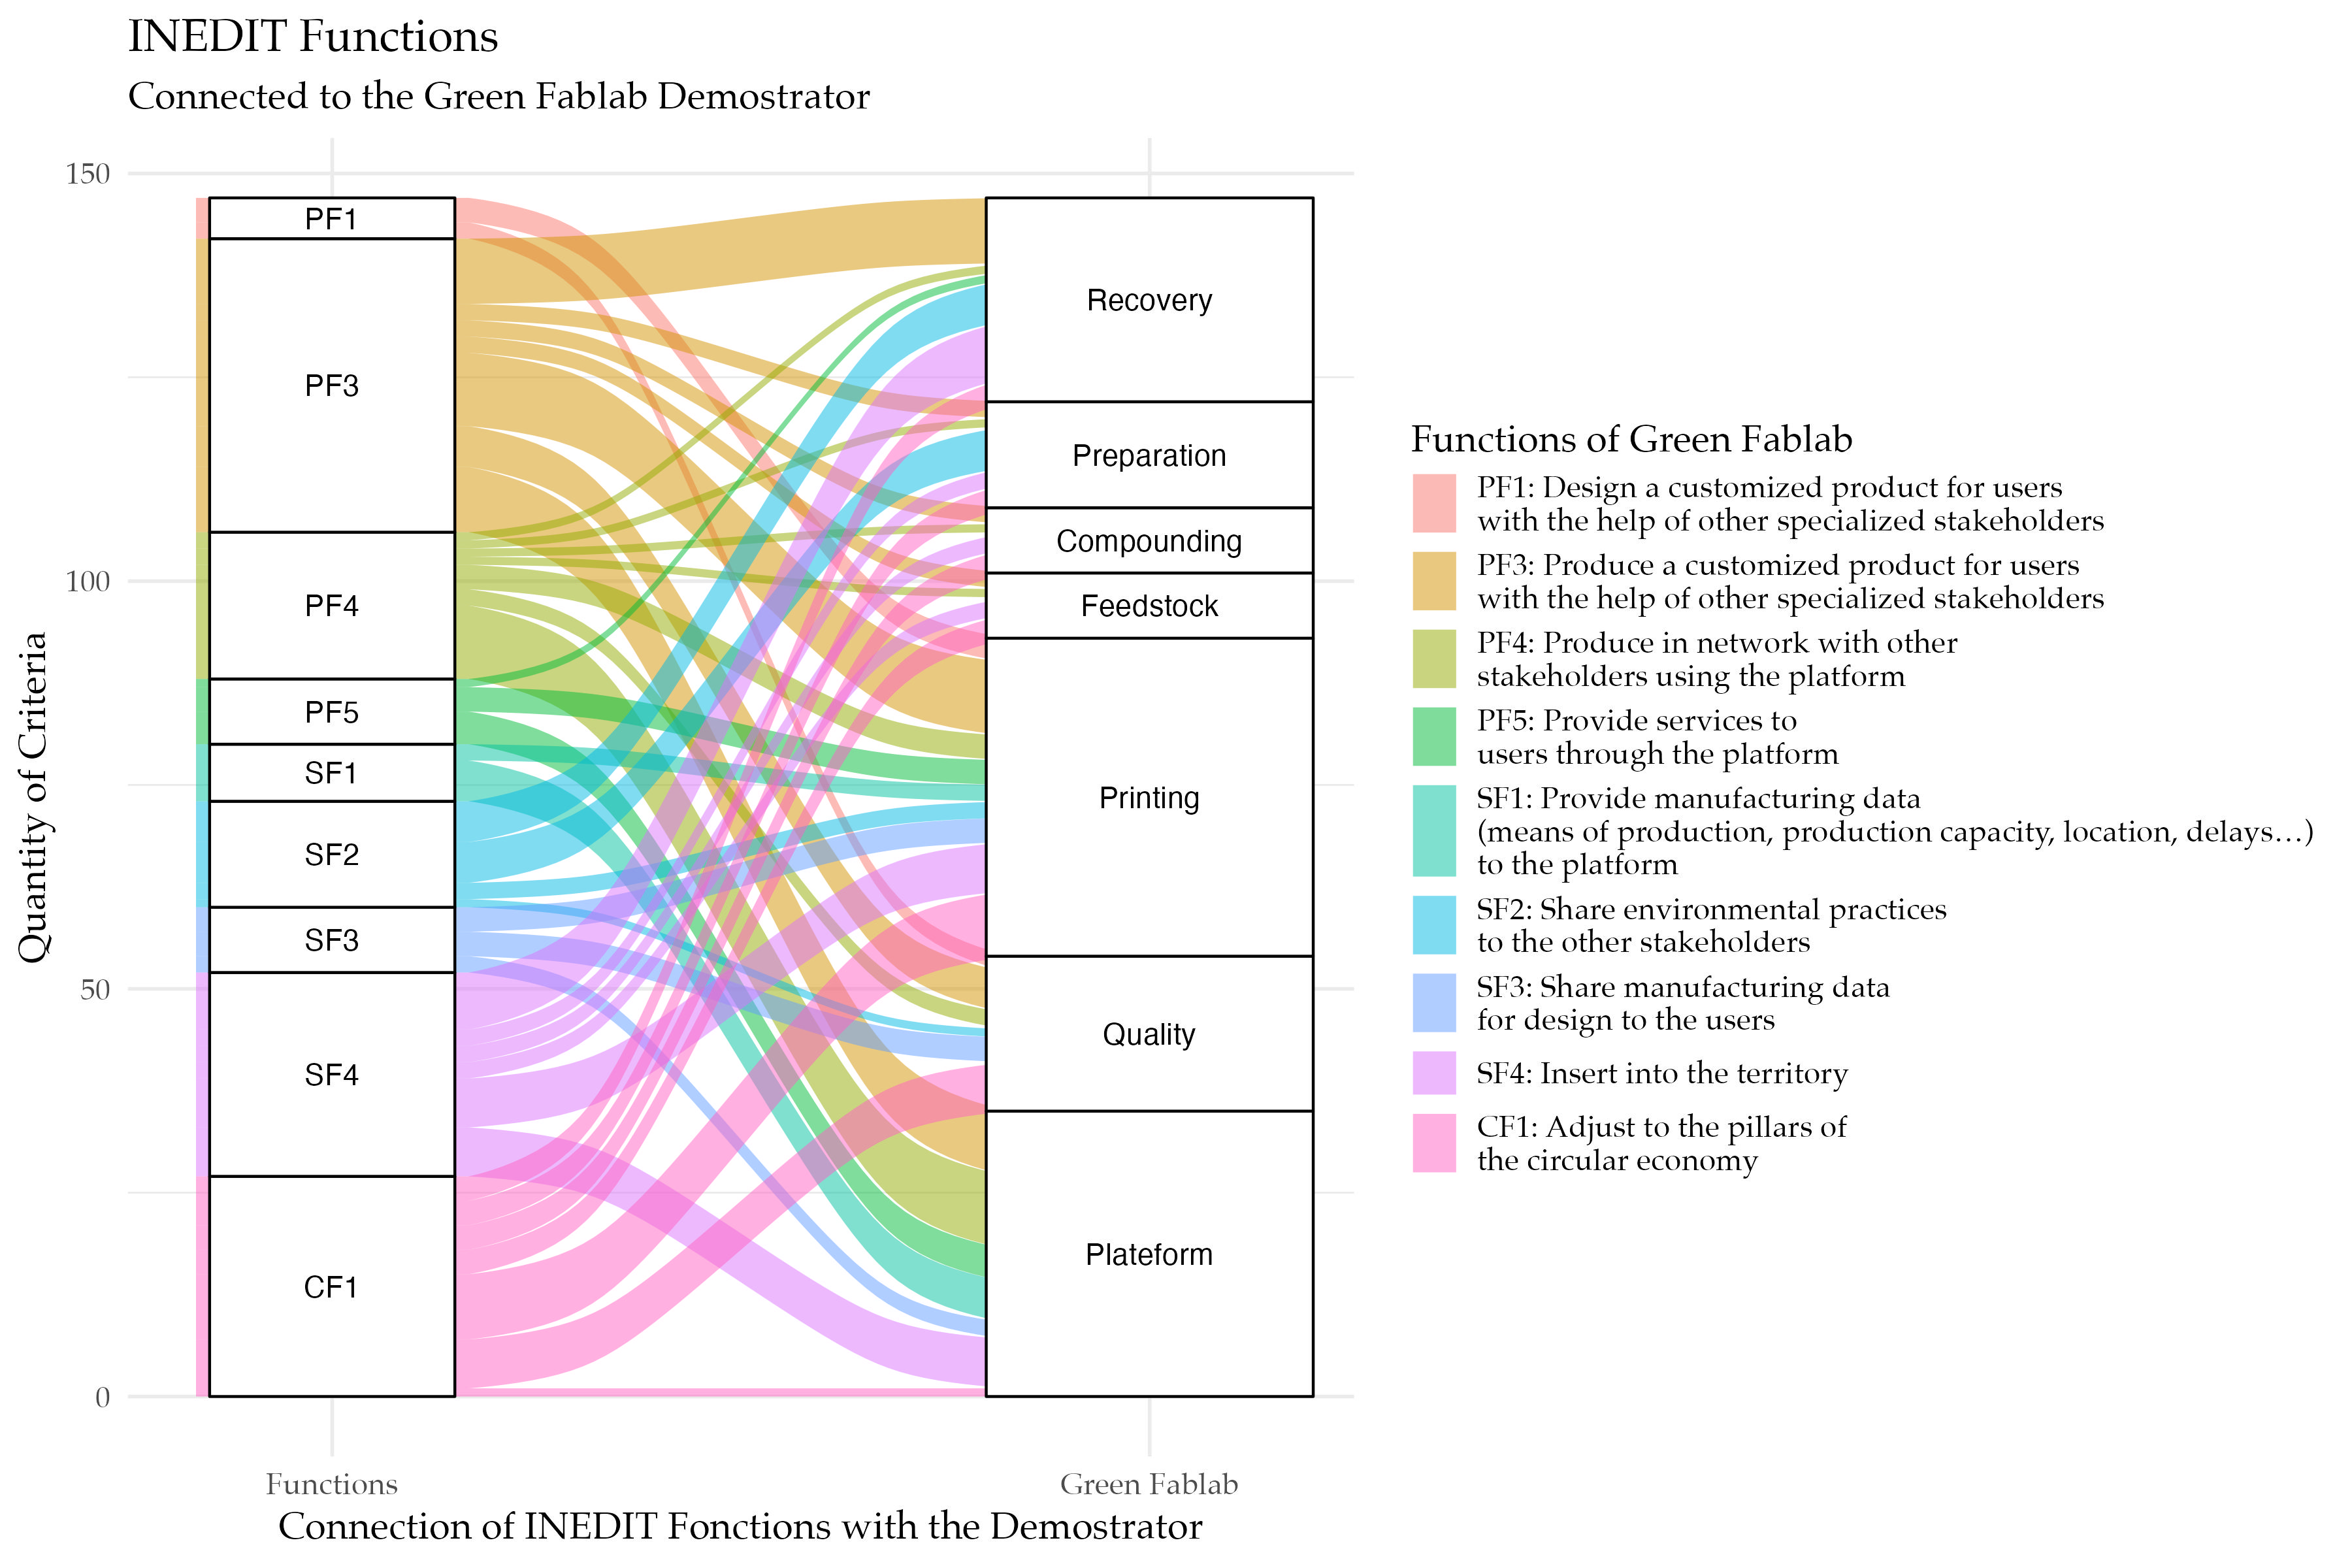
\includegraphics[width=0.95\textwidth,height=\textheight]{figures/Sankey-GF-Global.jpg}

}

\caption{\label{fig-dram}Connection of the 'Green Fablab Use case with
the Open Manufacturing Demonstration Facilities (OMDF) functions}

\end{figure}

\hypertarget{hypothesis-of-ul-case-for-deployment-in-reality}{%
\subsubsection{Hypothesis of UL case for deployment in
reality}\label{hypothesis-of-ul-case-for-deployment-in-reality}}

The implementation of the Green Fablab needs to be done considering
certain assumptions and simplifications to reduce the complexity of this
socio-technical system. The following assumptions were assumed in terms
of geographical scale, material recollection and manufacturing aspects:

\begin{itemize}
\item
  From a material perspective, only certain types of plastic wastes are
  considered. Specifically, Polyethylene terephthalate (PET), High
  density Polyethylene (HDPE), Polypropylene (PP) and Polylactic Acid
  (PLA). The major reason is from the technical perspective relies on
  the availability of these materials at the local area around the
  physical demonstrator.

  \begin{itemize}
  \item
    PLA is one of the most used plastics in 3D printing. Thus, as
    plastic waste source, PLA waste can be found from printed prototypes
    or 3D printed parts discarded.
  \item
    HDPE is one of ???
  \item
    PET
  \end{itemize}
\item
  The sorting, separation and cleaning process of plastics wastes are
  critical processes of the recycling. Therefore, this he recycling
  system considers t as a high because the collected material
  corresponds to a non-contaminated waste. For example, discarded 3D
  printing parts used for prototyping.
\item
  From a geographical point of view, only plastic waste collected from
  the smart collectors was considered. Nevertheless, as MVP use case
  demonstrator, this model can be extrapolated to schools and high
  schools in the Lorraine region (France) have been considered, and the
  route of recovery and delivery considered is obtained in the work of
  (\protect\hyperlink{ref-Santander2020}{Santander et al., 2020}).
\end{itemize}

The 3D printing activities carried out in these establishments have a
specific purpose of making product prototypes and mock-ups, which allow
to generate testing activities, design evaluations, functional
evaluations, corrections. Therefore, after a short lifetime, 3D printing
can be a source of significant amounts of plastic waste due to printed
parts that do not possess the desired quality, unused raw materials, or
products that have already fulfilled their life cycle
(\protect\hyperlink{ref-Alexandre2020}{\textbf{Alexandre2020?}})

\hypertarget{technical-characterization-of-the-3d-printing-of-recycled-demonstrator}{%
\subsection{Technical characterization of the 3D printing of recycled
demonstrator}\label{technical-characterization-of-the-3d-printing-of-recycled-demonstrator}}

\hypertarget{recovery-i}{%
\subsubsection{Recovery I}\label{recovery-i}}

The first step in the implementation of the Green Fablab OMDF is the
activity of \emph{Recovery I}. This phase aims to establish a minimal
baseline logistic operations to consider to collect the plastic wastes
to be recycled in the process. In the scientific literature, the
recovery is one of the main activities to considered in the recycling
process given that this structures a supply chain that certainly is
variable (i.e.~in function of the public support to sort the material in
the specific points of collection). This process is the first step to
create a closed-loop supply network approach for the distributed
manufacturing (\protect\hyperlink{ref-Santander2020}{Santander et al.,
2020}).

The collection tasks consists of collecting plastic waste at different
established points, which are then transported to a treatment center
where it is recycled. The collection and recycling process aims to
generate a recycling micro-network at the local level (neighborhood
scale), which allows the recovery and revaluation of plastic waste
through 3D printing. This allows to save impacts related to the
traditional treatment of plastic waste, as well as to increase the
recycling capacity in the city, giving more independence over the
recycling process. Figure~\ref{fig-recovery} illustrates the process
model considered.

\begin{figure}[H]

{\centering 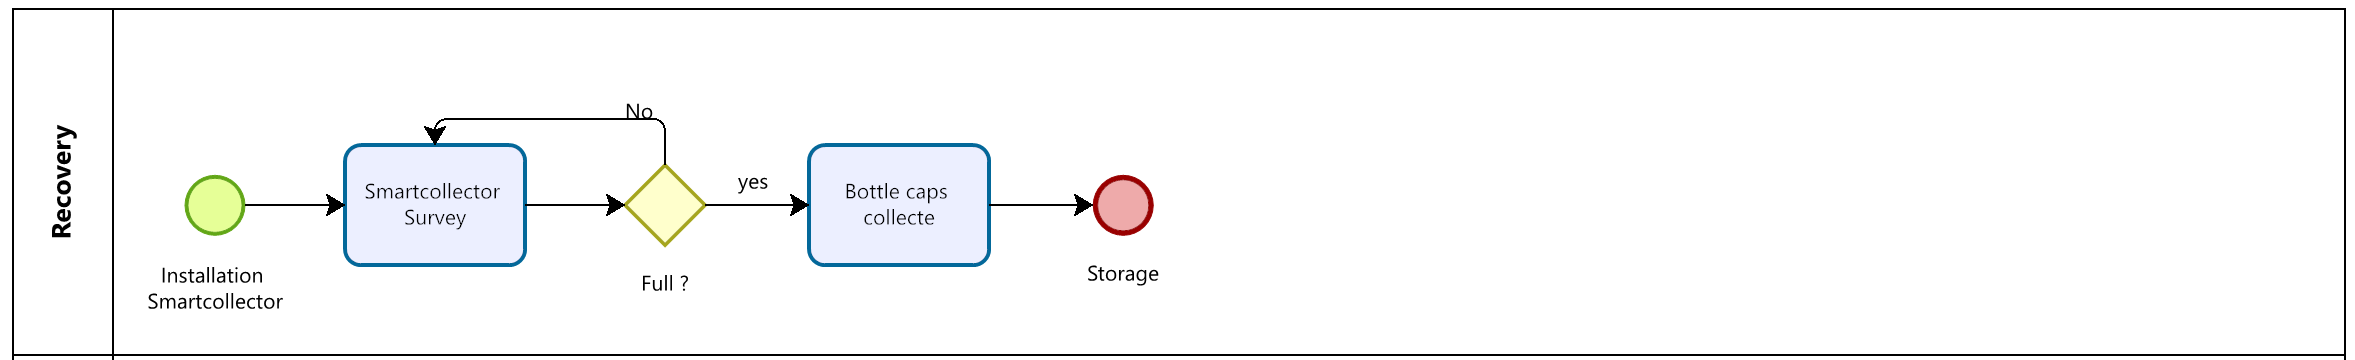
\includegraphics{figures/Recovery.png}

}

\caption{\label{fig-recovery}Recovery processus of the Green Fablab}

\end{figure}

The main difficult relies in the pertinent identification and the
quality state of the plastic waste. Therefore, in the framework of the
INEDIT project, the UL case demonstrator developed a ``smart collector
prototype'' as illustrated in the Figure~\ref{fig-smart-collector}. The
complete documentation of the technical device can be found in the
following open access reference
(\protect\hyperlink{ref-gabriel2023}{Gabriel and Cruz, 2023}). Given the
possible implementation in other contexts, the source files are shared
in open-source repository with the purpose that open communities to take
advantage the experiences developed at the Université de Lorraine.
Eventually, the open communities can propose improvements and better
versions.

\begin{figure}[H]

{\centering 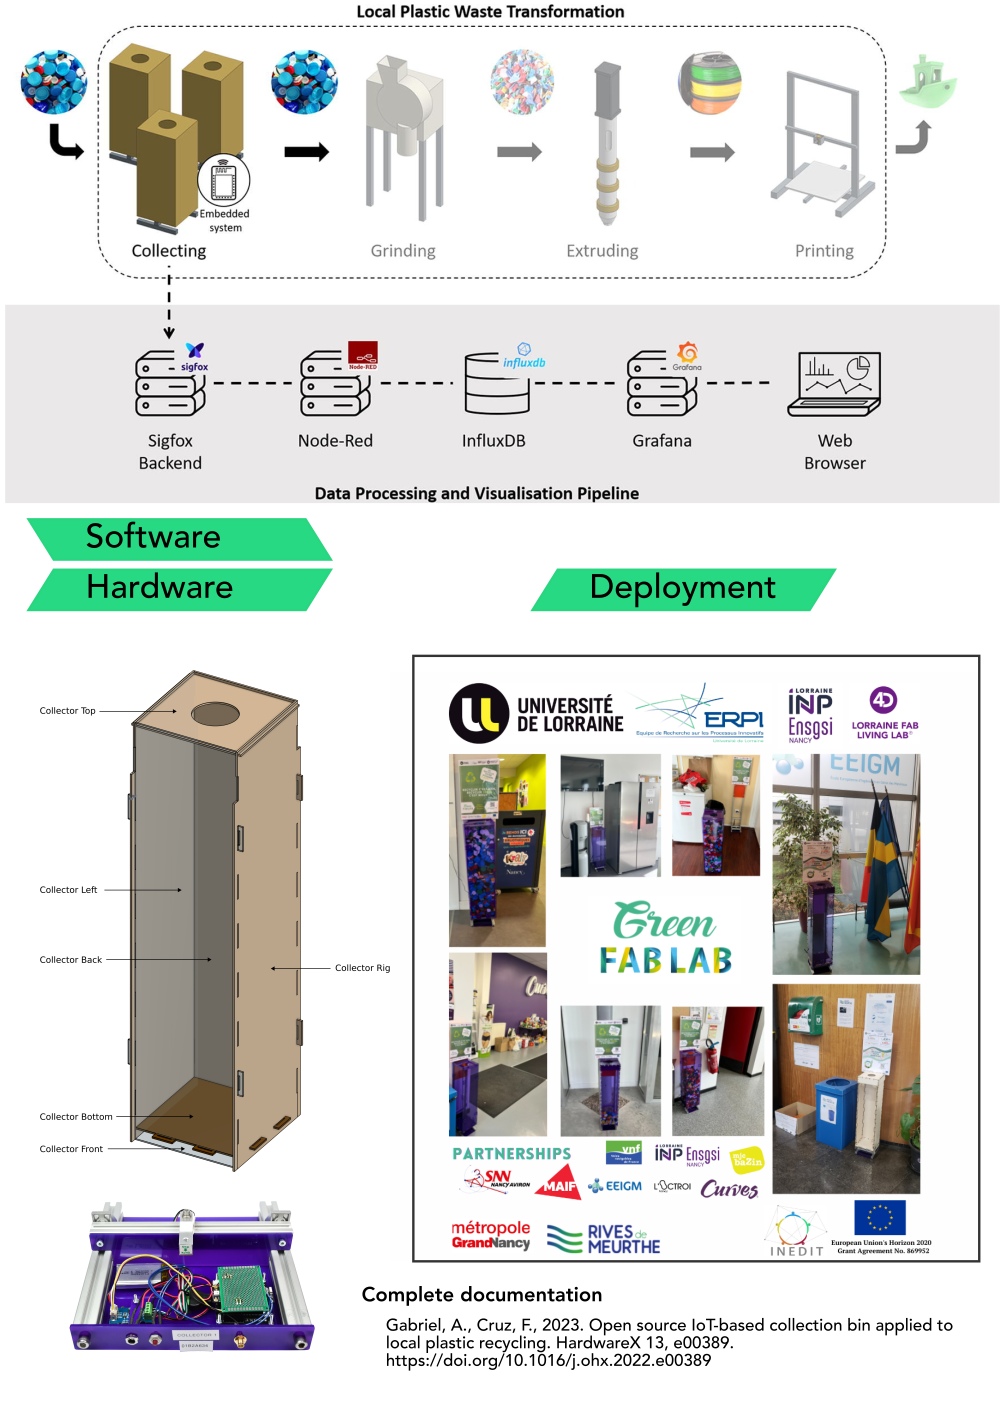
\includegraphics[width=4.16667in,height=\textheight]{figures/SC/Abstract.png}

}

\caption{\label{fig-smart-collector}Description of the developed Smart
collector}

\end{figure}

This is a relevant strategy given the cross-line of Industry 4.0 and
circular economy, which is opening up fields such as smart waste
management systems options to improve the effectiveness of different
materials, including plastic waste
(\protect\hyperlink{ref-Ranjbari2021}{Ranjbari et al., 2021}) using
information technology tools with the advent of the Internet of Things
(IoT) Rejeb et al. (\protect\hyperlink{ref-rejeb2022}{2022}). Smart
waste management system (SWMS) consists of public garbage collectors
with embedded technology that is used to monitor real-time level of
garbage bins in public places (\protect\hyperlink{ref-Bano2020}{Bano et
al., 2020}). The interest of this system is to optimize the path for the
garbage collecting van that eventually reduces fuel cost. However, this
work is mainly based on simulation. Therefore, there is an avenue to
simplify experimentation in this domain using common open-source
technology (hardware and software)
(\protect\hyperlink{ref-Pearce2009}{Pearce and Mushtaq, 2009}) to
implement projects that require heavy infrastructure such as routers and
a gateway to deploy in the territory.

The main functional requirement of the smart collector is to collect and
provide data about plastic waste production in order to design a local
and distributed recycling chain of value. However, the smart collector
may be used in various use cases such as:

\begin{itemize}
\tightlist
\item
  Monitoring the quantity of any other product that is collected over a
  large area.\\
\item
  Generating data about behavior to more precisely dimensions public
  infrastructure.\\
\item
  Monitoring the transformation and recycling process inside the
  transformation unit to follow the state and quantity of raw material
  and final product.\\
\item
  Initiating a digitization process in the waste management process as
  the information system element present here is flexible and commonly
  used in various types of projects.
\end{itemize}

The device uses a controller compatible with batteries and use WAN
technology to avoid the deployment of routers for data acquisition.
Although using various types of sensors allows us to achieve better
results (\protect\hyperlink{ref-Catania2014}{Catania and Ventura, 2014})
by crossing data, the main indicator remains the weight.

The process illustrated by the \textbf{?@fig-abstract} can be described
in the as follows:

\begin{enumerate}
\def\labelenumi{\arabic{enumi}.}
\item
  \textbf{Smart Collector installation}: The first step is to identify
  the main actors in the neighborhood through meetings, visits and
  interviews in order to propose integration into the recycling network
  by installing a smart collector on their premises.
\item
  \textbf{Supervision}: The monitoring is done through a dashboard that
  provides direct information sent by the smart collector. This allows
  to know the weight of each installed smart collector, allowing to have
  an approximation of its degree of occupancy.
\item
  \textbf{Receiving and storing plastic waste}: The storage area must be
  organized and functional with respect to the needs of the
  demonstrator.
\item
  \textbf{Plan and execute the collection}:
\end{enumerate}

In the scientific literature, the reverse logistic and closed loop
supply chains have been extensively studied in the scientific
literature. For instance,
(\protect\hyperlink{ref-Santander2021}{\textbf{Santander2021?}})
evaluated the benefits of a near loop and closed loop recycling network
focused on additive manufacturing, mainly producing recycled filament.
The main results show an economic and environmental benefit of sourcing
filament from recycled plastic rather than purchasing exported virgin
filament.

\hypertarget{preparation-ii}{%
\subsubsection{Preparation II}\label{preparation-ii}}

The second phase of the corresponds to the actions and processes to
identify, separate, sort, size reduce and clean waste plastic to
guarantee with the purpose to obtain feedstock material that is adequate
for the distributed recycling process.

The plastic waste preparation process aims to conditioned the collected
plastic to the requirements of 3D printing. For this process 3 main
sub-processes are considered:

\begin{itemize}
\item
  \textbf{Identification and Sorting}: These two processes aim to
  identify the type of plastic given the regular standard for the
  polymer industry. The process of identification and separation of
  plastics is done manually and allows to separate the plastics that can
  be used as raw material for further production processes.
\item
  \textbf{Cleaning}: This process is aims to remove the traces of any
  other substance that may be present in the plastic waste. In this way
  the processing machines will not be exposed to possible anomalies
  linked to material impurities.
\item
  \textbf{Size reduction}: The size reduction process is carried out to
  possible obtain an adequate granulometry. This process allows to adapt
  the plastic waste for the direct injection process and/or the
  extrusion process.
\item
  \textbf{Drying phase}: This step prevents the formation of bubbles in
  the recycled material when it is melted during the following extrusion
  or densification step
  (\protect\hyperlink{ref-Niaounakis2013}{\textbf{Niaounakis2013?}}).
  Moreover, complete elimination of water prevent hydrolytic
  decomposition of the molecular chains during the melting or
  plasticization, so that the treated material has to be as dry as
  possible.
\end{itemize}

\hypertarget{compounding-iii}{%
\subsubsection{Compounding III}\label{compounding-iii}}

The \emph{Compounding} phase is related to the operation, strategies in
the development of composite materials using recycled feedstock intended
to be use in a printing process. There have been several literature
reviews about the technical aspect of composite materials in the
additive manufacturing context Mohan et al.
(\protect\hyperlink{ref-Mohan2017}{2017}).

Special attention has been paid on material extrusion technologies in
the production of polymer/composite feedstocks as it is economical,
environmentally advantageous and adaptable to flexible filament material
(\protect\hyperlink{ref-Singh2017}{Singh et al., 2017}). For example,
Mohan et al. (\protect\hyperlink{ref-Mohan2017}{2017}) presented a
review on composite materials and process parameters optimisation for
the fused deposition modelling (FDM) process for improving the
mechanical properties (i.e.~tensile strength, fatigue). Brenken et al.
(\protect\hyperlink{ref-Brenken2017}{2018}) reported a detailed summary
of mechanical properties of printed parts for different composite
material for fused filament fabrication. Five majors strategies are
elucidated from the literature review such as:

In the context of the Green Fablab demonstrator of INEDIT project, the
focus is to study the 1) mono-recycled material and 2) the
virgin-recycled blend material. The development of recycling niches of
mono-material where the additive manufacturing can be implemented is key
to study. Different studies in laboratory conditions have been made to
show the technical feasibility of recycling. They include HDPE Kreiger
and Pearce (\protect\hyperlink{ref-Kreiger2013}{2013}), Biomass-derived
poly(ethylene-2,5-furandicarboxylate) (PEF)
(\protect\hyperlink{ref-Kucherov2017}{Kucherov et al., 2017}), PLA
(\protect\hyperlink{ref-CruzSanchez2017}{Cruz Sanchez et al., 2017}),
Linear Low Density Polyethylene (LLDPE)/ low density polyethylene
(LDPE), (\protect\hyperlink{ref-Hart2018}{Hart et al., 2018}),
thermoplastic elastomer (TPE) (\protect\hyperlink{ref-Woern2017}{Woern
and Pearce, 2017}). In fact, Hart et al.
(\protect\hyperlink{ref-Hart2018}{2018}) demonstrated the reconstitution
of residual polymeric packaging waste from Meals-Ready-to-Eat (MREs)
generated by soldiers around the world into additively manufactured
appliances. One conclusion of these studies is the positive technical
use of recycled mono-material for additive manufacturing purposes.

However, it has to be highlighted that one major assumption of these
studies relies in that the material used is already sorted, cleaned and
using a same type of discarded product. For INEDIT project, the interest
is to take into account the inner variability that could be in the
recovery process, concerning the type of material given the fact, while
there are seven types of recycling symbols for each type of polymer, one
major constraint in the current systems is that each manufacturing
company have a patented use of the additive in the polymer matrix, in
order to fulfil its initial function of the product.

\hypertarget{feedstock-iv}{%
\subsubsection{Feedstock IV}\label{feedstock-iv}}

The Feedstock III phase refers to the processes in order to transform
the plastic waste into usable material material for the fabrication
stage. Two outputs are seen in this etape: 1) the filament feedstock and
2) the pellet feedstock. The use of filament or pellet material are in
coherence with the machine process used in the fabrication (cf section
4.4.5). The figure XX present the modeling of the process:

The filament and pellet production process makes it possible to produce
the necessary raw material from plastic waste. The production of these
intermediate products allows the use of different technologies related.
Before using these products (filaments and pellets) it is necessary to
carry out evaluation tests to assess the geometrical characteristics
that are necessary in the printing process.

Figure XX and table present the technical characteristics of the
material equipement

\hypertarget{fabrication-process-technological-mix-to-valorize-the-recycled-material}{%
\subsubsection{Fabrication process -- Technological mix to valorize the
recycled
material}\label{fabrication-process-technological-mix-to-valorize-the-recycled-material}}

In this step, the major output is the valorisation of the plastic waste
material using different two alternative paths: 1) Desktop injection
process, and 2), 3D printing process. As matter of the validation of the
demonstrator at TRL 6 level, the ambition of the demonstrator in the
INEDIT project is to experiment and prove a technological ecosystem mix
that seeks to valorise in a distributed approach different plastics for
different purposes and stakeholders. Therefore, the initial choice is
these two paths to create objects injected and 3D printed parts that are
useful to the local ecosystem of the demonstrator. The technologies are
presented in the following paragraphs.

\hypertarget{desktop-injection-moulding}{%
\paragraph{Desktop injection
moulding}\label{desktop-injection-moulding}}

Injection moulding is one of the most used technique to form plastic
materials.\\
The major point in the `Green Fablab' case is to propose a manual
recycled aspect to possible reuse the plastic waste into sheet

\hypertarget{d-printing-process-fused-filament-granular-fabrication-fff-fgf}{%
\paragraph{3D printing process: Fused Filament \& Granular Fabrication
(FFF \&
FGF)}\label{d-printing-process-fused-filament-granular-fabrication-fff-fgf}}

In the era of the additive manufacturing technology, without a doubt,
the material extrusion-based systems such as the fused filament
fabrication (FFF) has been one of the prominent processes. In fact, the
technological development of open-source 3D printers is creating more
affordable Additive Manufacturing (AM) machines for society in different
applications. It provides the possibility of mass diffusion of this
technology, and consequently, AM is being recognised as a disruptive
that could up-end the last two centuries of approaches to design and
manufacturing Birtchnell and Urry
(\protect\hyperlink{ref-Birtchnell2013a}{2013}).

In the Green Fablab demonstrator, we have two types of material-based
systems:

\begin{enumerate}
\def\labelenumi{\arabic{enumi})}
\tightlist
\item
  Fused filament fabrication (FFF) and 2) Fused Granular Fabrication
  (FGF):
\end{enumerate}

\begin{figure}

\begin{minipage}[t]{0.50\linewidth}

{\centering 

\raisebox{-\height}{

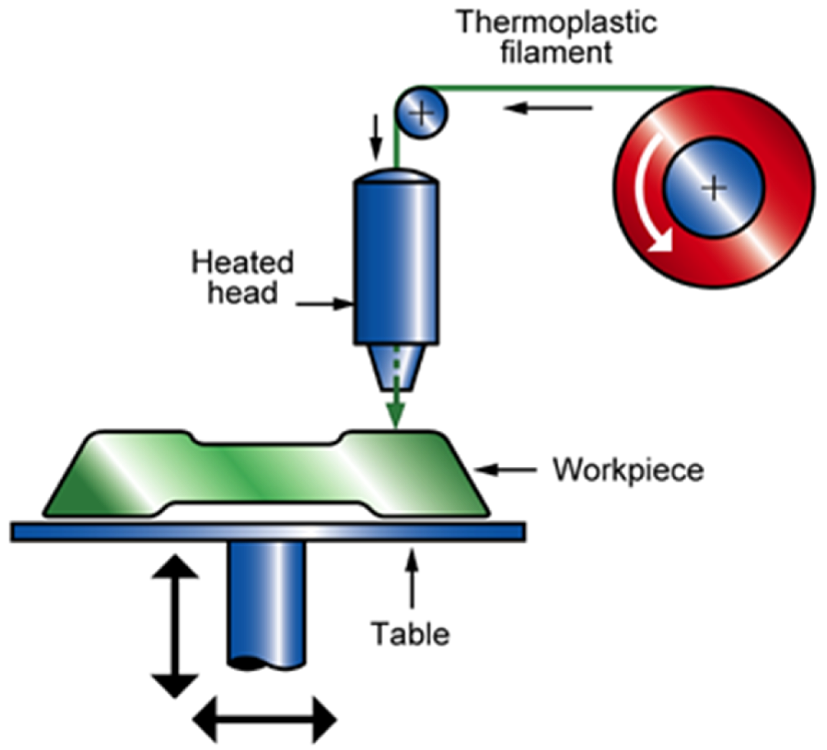
\includegraphics[width=2.08333in,height=\textheight]{figures/FFF-00.png}

}

}

\subcaption{\label{fig-fff}Fused filament fabrication -FFF- principle}
\end{minipage}%
%
\begin{minipage}[t]{0.50\linewidth}

{\centering 

\raisebox{-\height}{

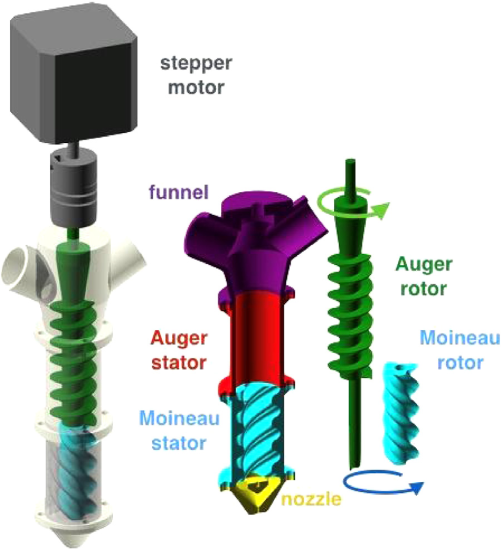
\includegraphics[width=2.08333in,height=\textheight]{figures/Canessa2017.png}

}

}

\subcaption{\label{fig-hanno}Fused granular fabrication -FGF- principle}
\end{minipage}%

\caption{\label{fig-smart-collector}Additive manufacturing of
material-extrusion based systems}

\end{figure}

The filament fabrication was developed and patented in 1989 by Scott
Crump as \emph{Fused Deposition Modelling}, and since 2009, the
technology became open source
(\protect\hyperlink{ref-Crump1992}{\textbf{Crump1992?}}), known as Fused
Filament Fabrication, to establish the difference between the registred
mark. A schematic representation of this technology is presented in
Figure~\ref{fig-fff}. This process usually uses thermoplastic polymer
filaments that are heated until a temperature slightly higher than the
melting temperature at the nozzle of the machine, reaching a semi-liquid
state. At this point, the polymer is extruded on the platform to create
the first layer of the object and after that, the polymer continues to
be printed on top of the previous layer, so that, filament fuses with
the previous layer and then is solidified at room temperature after
printing Cruz Sanchez et al.
(\protect\hyperlink{ref-CruzSanchez2017}{2017}).

At the green Fablab

\begin{figure}[H]

{\centering 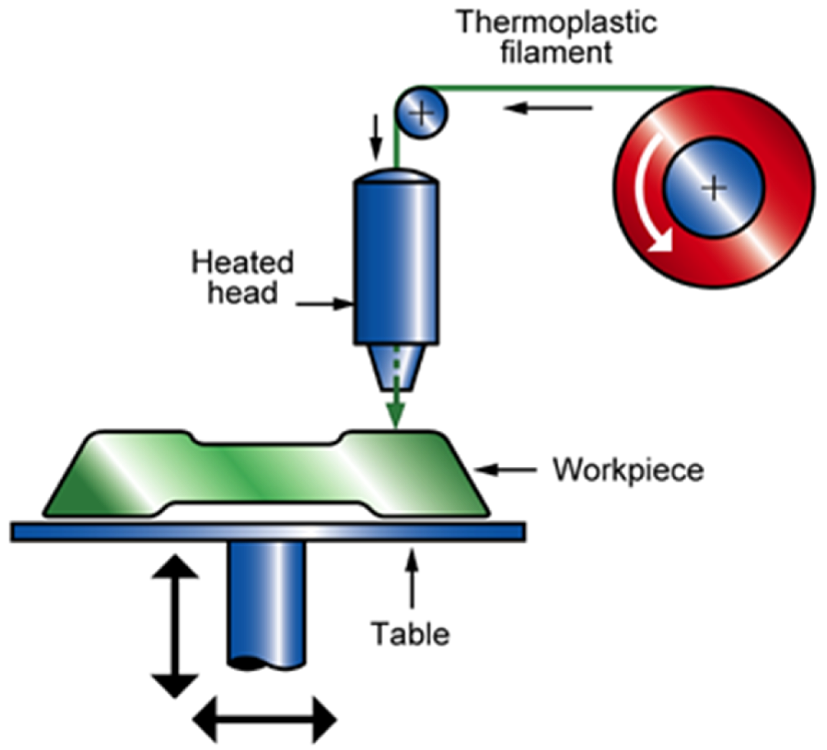
\includegraphics[width=2.08333in,height=\textheight]{figures/FFF-00.png}

}

\caption{\label{fig-fff}Fused filament fabrication -FFF- principle}

\end{figure}

For the

On the other hand, the Fused Granular Fabrication is a direct extrusion
systems of pellets is a key technical advancement to facilitate the use
of recycled material in the printing process. Volpato et al.
(\protect\hyperlink{ref-Volpato2015}{2015}) describes the development of
a piston driven extrusion head that can extrude polypropylene granules
into a filament. The head was designed to minimize the volume of
material fused during the extrusion process and reduce the effect of
material degradation. Canessa et al.
(\protect\hyperlink{ref-Canessa2017}{2017}) developed a mini extruder
for pellets or granules of recycled plastic that can be used in a RepRap
FDM 3D printer for rapid prototyping. The use of Moineau pump technology
to add precise volumetric control to the extrusion of pellets opens
extraordinary new possibilities. It is important to mention that a
Moineau pump has to be coupled to a first stage Auger screw. This
ensures a continuous feed of melted plastic with-out inclusion of air
bubbles, since the Moineau pump itself cannot guarantee such condition.
However, it is also important to highlight that currently this
technology is the phase of laboratory experimentation and initial market
diffusion. The complexity

\begin{figure}

\begin{minipage}[t]{0.50\linewidth}

{\centering 

\raisebox{-\height}{

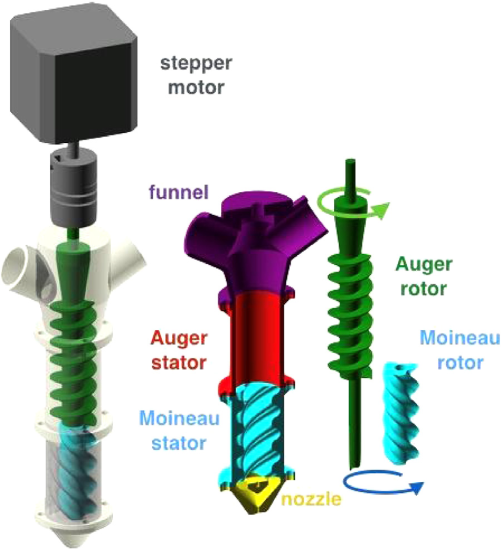
\includegraphics[width=2.08333in,height=\textheight]{figures/Canessa2017.png}

}

}

\subcaption{\label{fig-hanno}Fused granular fabrication -FGF- principle}
\end{minipage}%

\caption{\label{fig-smart-collector}Additive manufacturing of
material-extrusion based systems}

\end{figure}

This machine has a compressions screw which makes pellets or granules of
thermoplastic materials feasible to be 3D printed.

Gigabot X XL machine extruder has a long barrel with 3 heating elements
or zone which helps in uniformly melting and viscosity control of the
thermoplastic. T1 being the heating block near the nozzle while T2 being
in the middle of T1 and T3. Gigabot X XL is equipped with nozzle of
1.75mm diameter which provides good deposition rate. As 3D printing
smaller cross-section is very hard without a cooling system near the
nozzle {[}13{]},{[}14{]} therefore a cooling system was designed, 3D
printed using ABS material and installed onto the system Figure 1

\hypertarget{quality-assessment-vi}{%
\subsubsection{Quality Assessment VI}\label{quality-assessment-vi}}

The quality assessment phase is the process to assess the technical
feasibility of the recycled part.

\hypertarget{operationalization-of-dit-process-for-the-use-case}{%
\section{Operationalization of DIT process for the Use
Case}\label{operationalization-of-dit-process-for-the-use-case}}

\hypertarget{integration-of-the-3d-printing-recycled-plastic}{%
\subsection{Integration of the 3D Printing Recycled
Plastic}\label{integration-of-the-3d-printing-recycled-plastic}}

Explanation of the INEDIT project but focusing on the Open Manufacturing
Demonstration Facilities process

\begin{table}[H]
\centering\begingroup\fontsize{10}{12}\selectfont

\begin{tabular}[t]{>{\raggedright\arraybackslash}p{5cm}>{\raggedright\arraybackslash}p{10cm}>{\raggedright\arraybackslash}p{1.5cm}}
\toprule
Steps ID  & Steps Description  & Corresponding ID\_DIT process \\
\midrule
\cellcolor{gray!6}{STEP 1 - RECEIVE DESIGN AND SPECIFICATION } & \cellcolor{gray!6}{Information about materials, finish, colour, texture, etc. from the INEDIT platform are sent to the manufacturing centre chosen by the ERP module and the Sustainability Driven Orchestrator (SDO). The expected files to be imported are: CAD file of the object, colour and texture, technical requirements identified in the design phase. } & \cellcolor{gray!6}{7\_1 }\\
STEP 2 - VALIDATION OF THE TECHNICAL SPECIFICATIONS OF MODEL TO FABRICATE  & Furniture producers or FabLab with the support of 3D printing technical experts evaluate the printability (if the part can be printed with the available technology) as well as validate the design.  & 7\_2 \\
\cellcolor{gray!6}{STEP 3 - IDENTIFY LOCAL SOURCES OF PLASTIC WASTE } & \cellcolor{gray!6}{This step starts identifying local sources of plastic waste at least 2 km far from the production site. Designers and technicians will evaluate the quantity and quality of possible plastic wastes that could be used as secondary raw material. } & \cellcolor{gray!6}{9\_2 }\\
STEP 4 – PUT IN PLACE SMART COLLECTOR  & By using the Smart Collector developed by UL in the local areas (< 2 km) it is enabled to collect plastic waste from the sources identified before.  & 9\_6 \\
\cellcolor{gray!6}{STEP 5 - TRANSPORT WASTE MATERIAL TO THE RECYCLING FACILITIES } & \cellcolor{gray!6}{All the recycled plastic waste is collected and transported to the recycling facilities } & \cellcolor{gray!6}{9\_9 }\\
\addlinespace
STEP 6 - ADEQUATION AND PREPARATION OF THE MATERIAL, MATERIAL PRINTABILITY VERIFICATION  & The collected material has to be adequate in order to be utilised as recycled feedstock (sorting of usable material, cleaning, etc). The treated material needs to be tested and validated (evaluation on usage and printability).  & 10\_4 \\
\cellcolor{gray!6}{STEP 7 - PATH PLANNING–3D PRINTING } & \cellcolor{gray!6}{Path planning software generates the best printing strategy to reduce the material used and time. The high-tech solution developed by UL manufactures using at least 30\% of recycled plastic the product in the previously chosen manufacturing centre. } & \cellcolor{gray!6}{5\_1\_2 }\\
STEP 8 – POST PROCESSING  & If needed, a post-processing phase refines the product in terms of aesthetic quality in order to meet customer requirements. Some parts need to be assembled in the manufacturing site before shipping to the customer.  & 5\_1\_2 \\
\cellcolor{gray!6}{STEP 9 – TEST BY USE } & \cellcolor{gray!6}{The DIT innovation space enables the designer to test the just realized prototype, to ensure proper functioning in real conditions. } & \cellcolor{gray!6}{6\_1\_1 }\\
STEP 10 – RE-DESIGN AND AFFINATION OF FABRICATION  & If the test by use of the prototype fails, the failure is improved and corrected, repeating the process (re-involving the necessary stakeholders and the technologies used).  & 5\_2\_2 \\
\addlinespace
\cellcolor{gray!6}{STEP 11 – VALIDATION } & \cellcolor{gray!6}{The use case ends validating the product printed, first by the manufacturer and the designer, second by a responsible entity for verification of design feasibility that provides safety and environmental certification and lastly by the customer use (feedback). } & \cellcolor{gray!6}{6\_1\_2 }\\
\bottomrule
\end{tabular}
\endgroup{}
\end{table}

\hypertarget{step-1-receive-design-and-specification}{%
\subsection{Step 1 -- Receive Design and
Specification}\label{step-1-receive-design-and-specification}}

The first step in the reception of the design models and specifications
from the INEDIT platform. The starting point of this activity is the
reception of the respective documents that contains the 3D model to be
manufactured by the use case.

One of the outputs of the co-creation phase of INEDIT is the creation of
a first initial model that can be exploitable in the open manufacturing
process. In that way, the model is received taking into account the
specific requirements of the customer, and the required inputs to
determine if the technologies available in the demonstrated have the
capacity to produce the product. In the case that it cannot be produced,
it is necessary to notify immediately together with the arguments why it
cannot be produced and offer ways of improvement.

\hypertarget{step-2-validation-of-the-technical-specifications-of-model-to-fabricate}{%
\subsection{Step 2 -- Validation of the technical specifications of
model to
fabricate}\label{step-2-validation-of-the-technical-specifications-of-model-to-fabricate}}

In this step, the main purpose is to establish the criteria for the
validation specifications of the model to faricate.

In the case of the Green FabLab, three main criteria were established

\begin{enumerate}
\def\labelenumi{\arabic{enumi}.}
\tightlist
\item
  Concerning the dimmensions
\item
  Concerning the material
\item
  Concerning the printability
\end{enumerate}

\hypertarget{step-3-identify-local-source-of-plastic-waste}{%
\subsection{Step 3 -- Identify local source of plastic
waste}\label{step-3-identify-local-source-of-plastic-waste}}

This step seeks to establish a first network of plastic wastes source
from the local ecosystem. The task of the identification of local source
of plastic is fundamental as the first stage in the recovery process.\\
As illustrated in the Figure~\ref{fig-fedoua-00}, the methodological
approach included the following steps:

\begin{enumerate}
\def\labelenumi{\arabic{enumi}.}
\tightlist
\item
  Pre-diagnosis of the territorial context,
\item
  Identification of the actors,
\item
  Analysis of the actors' involvement and implementation of the smart
  collector, and finally,
\item
  Implementation \& monitoring.
\end{enumerate}

\begin{figure}[H]

{\centering 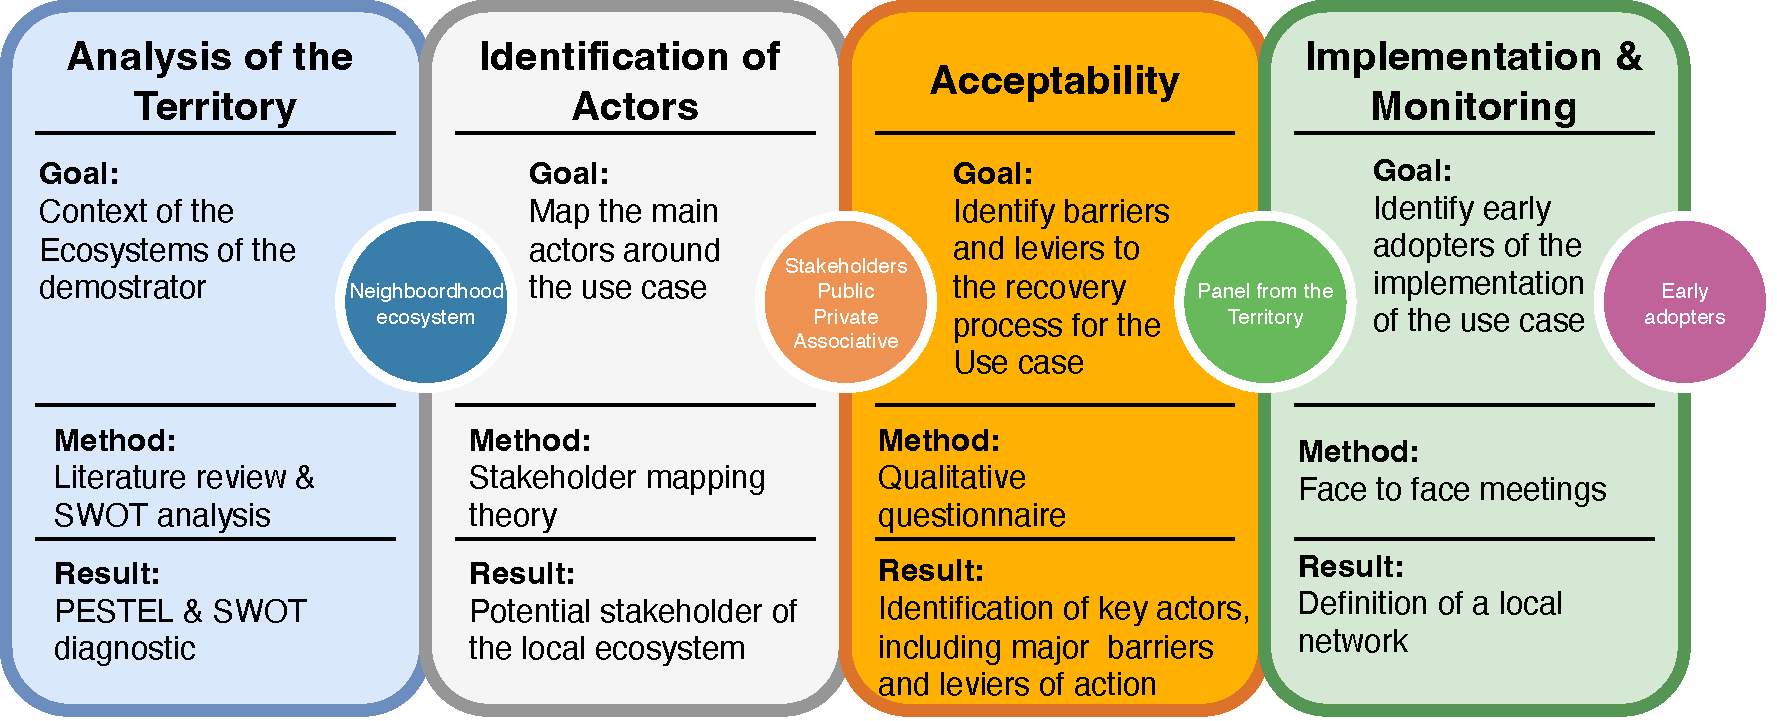
\includegraphics[width=0.9\textwidth,height=\textheight]{figures/Fedoua-00.pdf}

}

\caption{\label{fig-fedoua-00}Methodological steps for the
identification of local sources of plastic wastes}

\end{figure}

Regarding the pre-diagnosis phase, the purpose was to align the INEDIT
project with the territorial context. To do so, between XX-2021 and
YY-2022, the UL team had exchange with key actors of territorial
development agencies and associations (Annex XX for more details) and
the priorities in terms of sustainable development. The main output of
this phase was the establishment of an initial Swot-Pestel analysis for
the implementation of a local recycling network of plastic waste at the
neighborhood of Rives de Meurthe at Nancy.

Based on this first step, it was possible to identify relevant
stakehoders in the local ecosystems to inquire on the issue of plastic
wastes source. First, they needeed to be in a geographical range
perimeter (less than 2km around the Green Fablab) following the
observations of Santander et al.
(\protect\hyperlink{ref-Santander2020}{2020}). Limiting the geographical
perimeter of collection helps in the reduction of environmental impact
because of the reduction of transport impact. Second, the
diversification of the actor profile that can be sensibilized to the
participation of the collection (general public, employees, students)
and/or stakeholder's status (Public, Private, Associative) where the
smart collector can be deployed. These two elements were essential to
consider because the experimentation seeks to establish a baseline of
the recovery process given the uncertainties of participation of the
local context and the sensitization to the management of the plastic by
the general public.

\begin{figure}

\begin{minipage}[t]{0.50\linewidth}

{\centering 

\raisebox{-\height}{

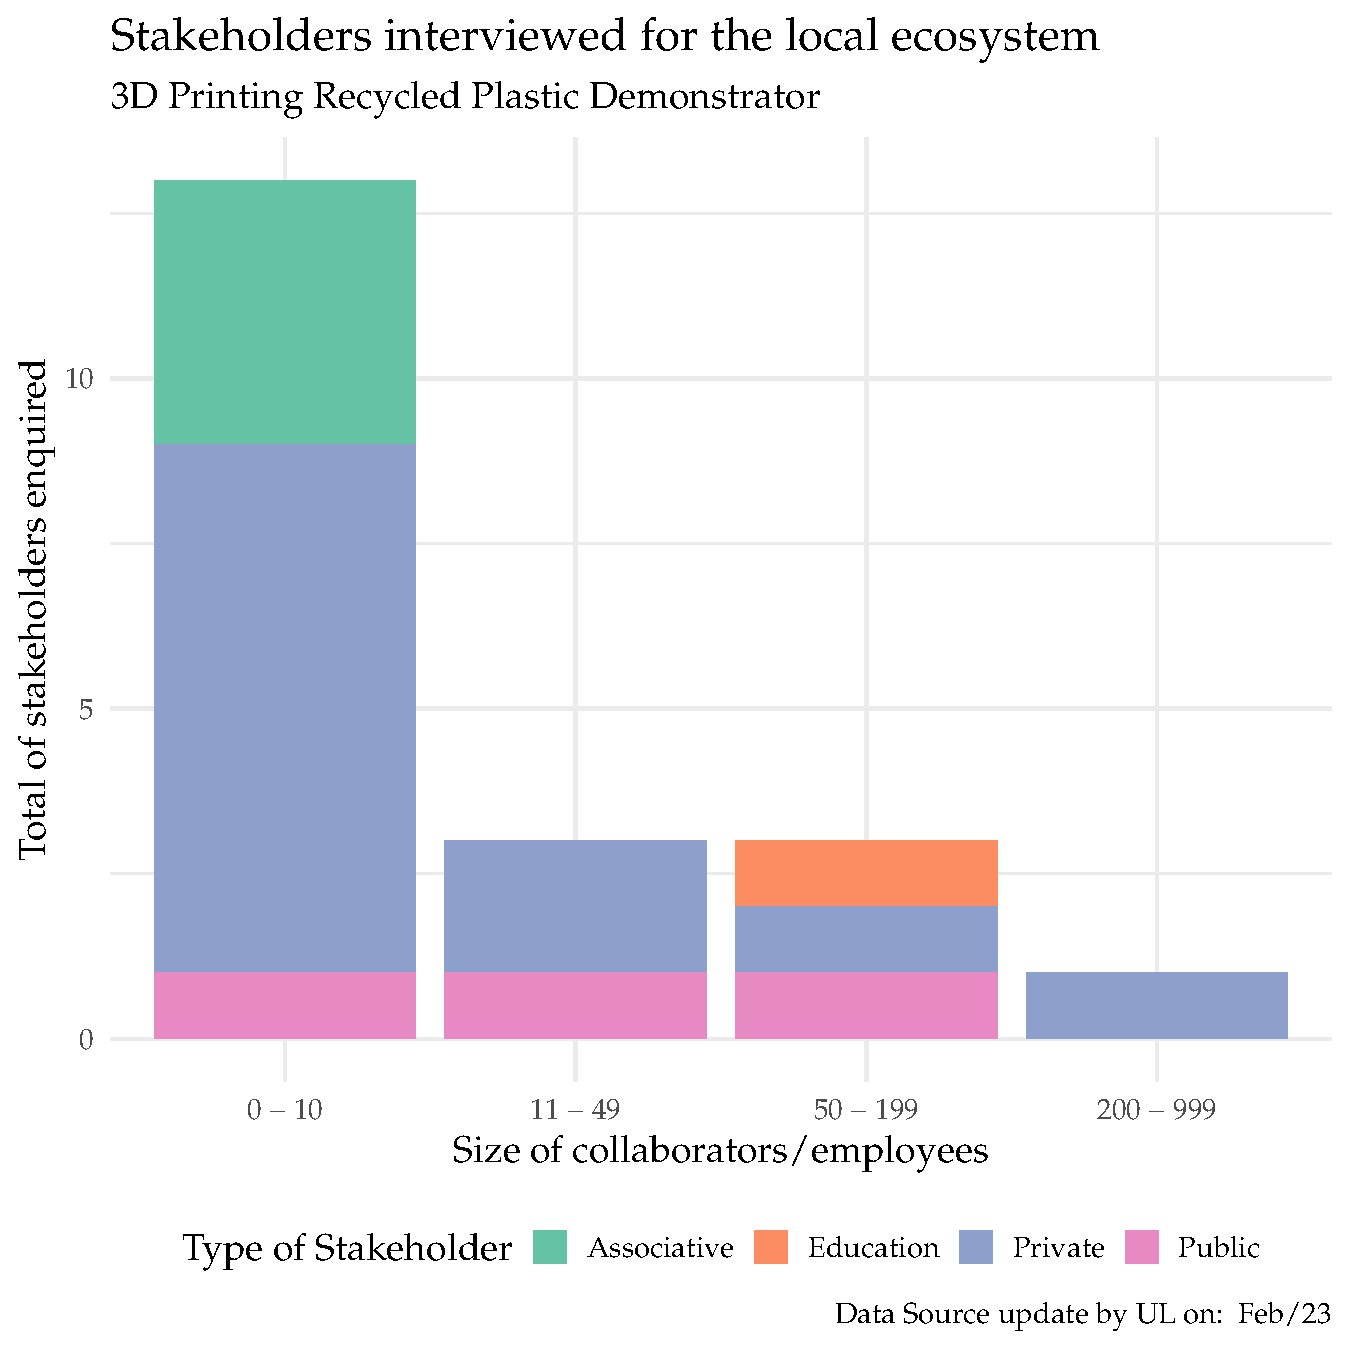
\includegraphics{figures/fedoua/Ecosystem-01.pdf}

}

}

\subcaption{\label{fig-ecosystem-00}Local ecosystem interviewed about
the implementation ofa 3D printing recycled demostrator}
\end{minipage}%
%
\begin{minipage}[t]{0.50\linewidth}

{\centering 

\raisebox{-\height}{

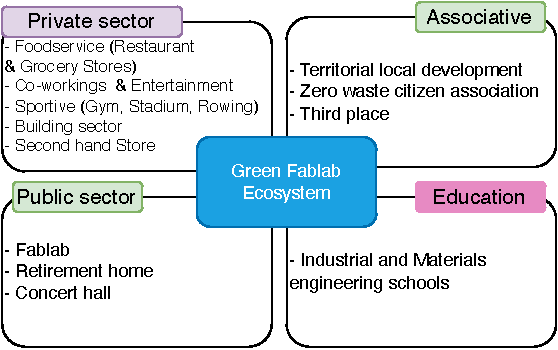
\includegraphics{figures/fedoua/Ecosystem-00.pdf}

}

}

\subcaption{\label{fig-ecosystem-01}Type of stakeholders for the}
\end{minipage}%

\caption{\label{fig-ecosystem}LOcal ecosystem enquired}

\end{figure}

A total of 23 actors were interviewed in the period of time of XX-2020 -
YY-2022, of which 21 by physical or telephone interview and 2 by
electronic questionnaire They were mainly companies (X\% small and Y\%
medium size), associative entities, academic sector. The diversity of
the public was an interesting criterion for the study. Participants in
the economic, cultural and social dynamics of the district through their
membership in the local association of economic actors of the territory.

The scope of activity of most of the respondents is local (at the level
of the neighborhood or city) which may reflect a strong territorial
anchoring and a commitment to local concerns and issues (waste
management, social welfare, local job creation\ldots). The majority of
their business decisions are made locally, which reduces the risk of
depending on the interests of entities outside the territory.

\begin{figure}[H]

{\centering 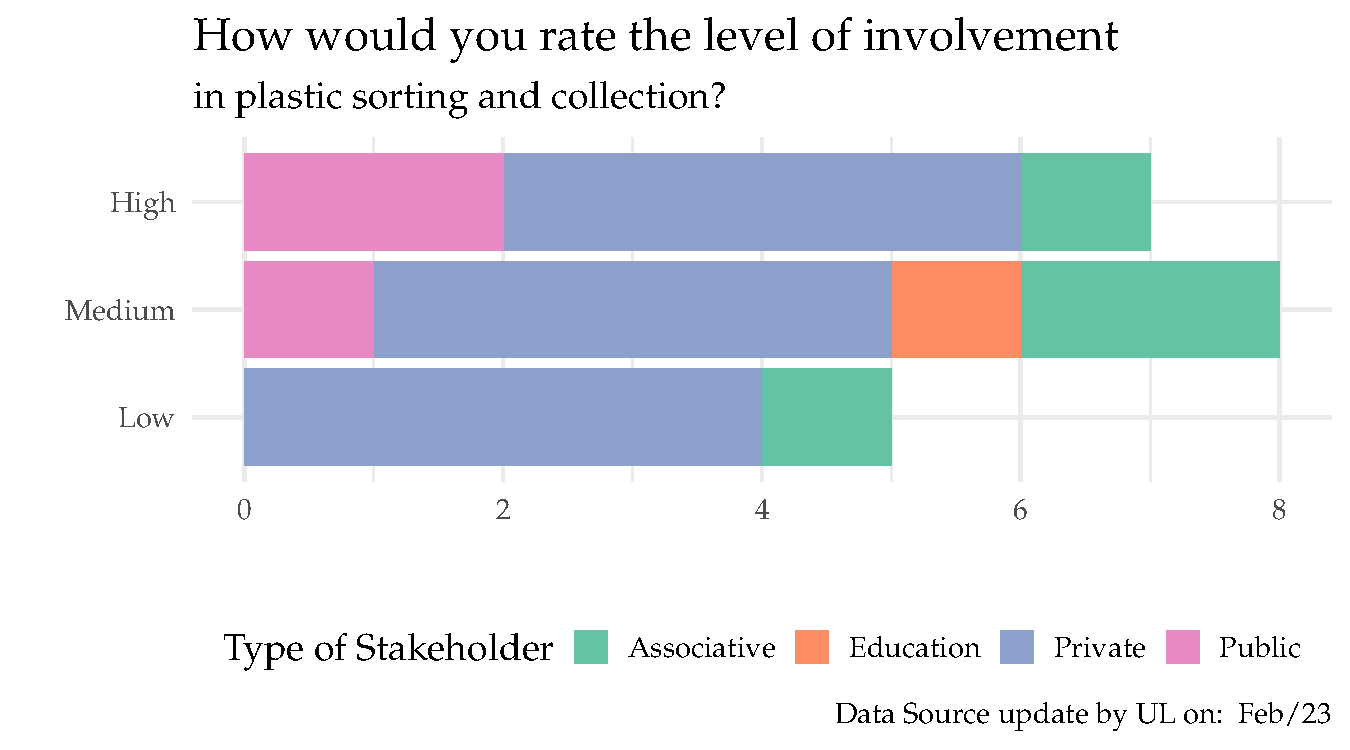
\includegraphics[width=0.9\textwidth,height=\textheight]{figures/fedoua/Acceptability-01.pdf}

}

\caption{\label{fig-acceptability-01}Local ecosystem interviewed about
the implementation ofa 3D printing recycled demostrator}

\end{figure}

To do this, we identified the role of each actor, then the sources of
plastic waste collection, and then identify the sources of 3D printing
and potential synergies with LF2L. In order to achieve these results, an
exchange with key actors in territorial development was necessary.

\begin{figure}[H]

{\centering 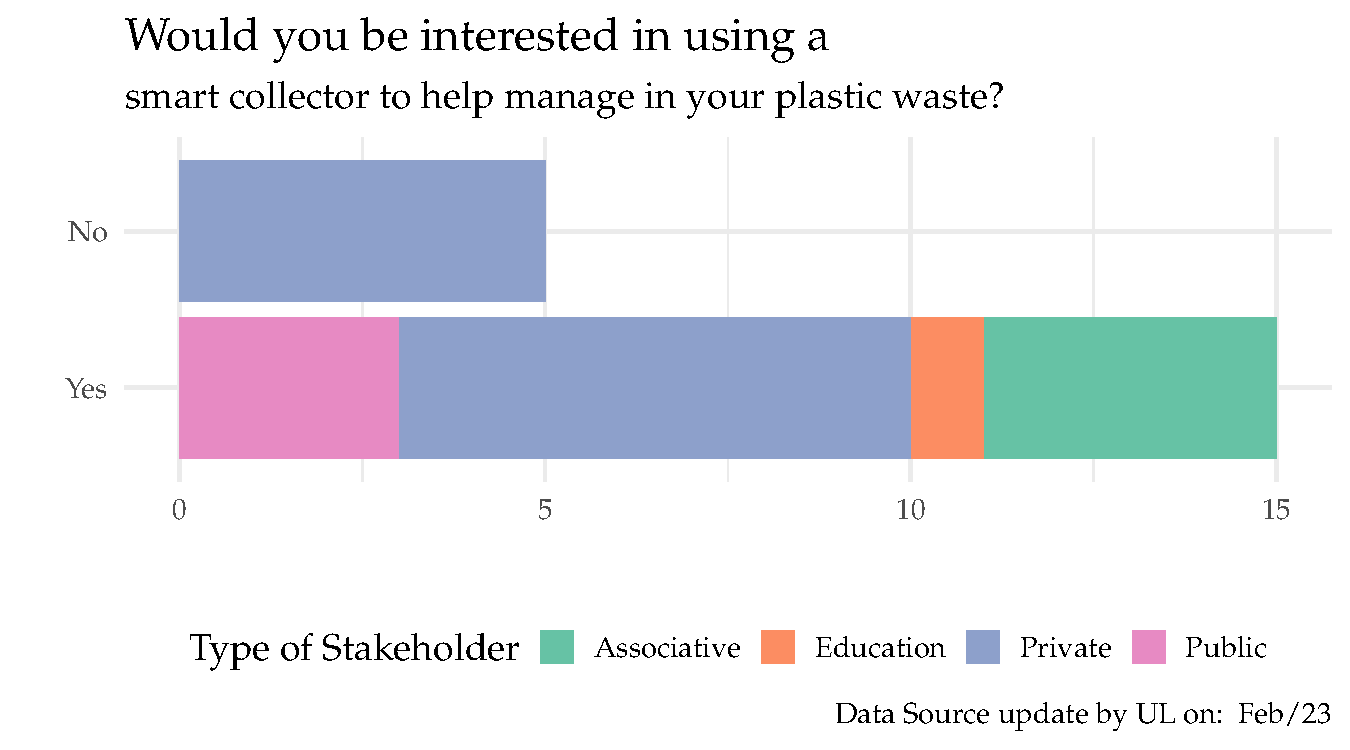
\includegraphics[width=0.9\textwidth,height=\textheight]{figures/fedoua/Acceptability-02.pdf}

}

\caption{\label{fig-acceptability-02}Acceptability of the possible use
of `smart collector' for the}

\end{figure}

Thanks to this approach, we have identified eigth collection sites at
the local territory for the deployment of the smart collector.

\hypertarget{step-4-put-in-place-smart-collectors}{%
\subsection{Step 4: Put in place smart
collectors}\label{step-4-put-in-place-smart-collectors}}

In this step the main purpose is the deployment of a set of \emph{smart
collectors} around the neighborhood. Figure~\ref{fig-sc-deployment}
presents the selected points around the Green FabLab for the
installation of the prototype. The smart collector is produced and
mounted manually. The specific details and step-by-step assemble process
can be found in the technical paper
(\protect\hyperlink{ref-gabriel2023}{Gabriel and Cruz, 2023}).

\begin{figure}[H]

{\centering 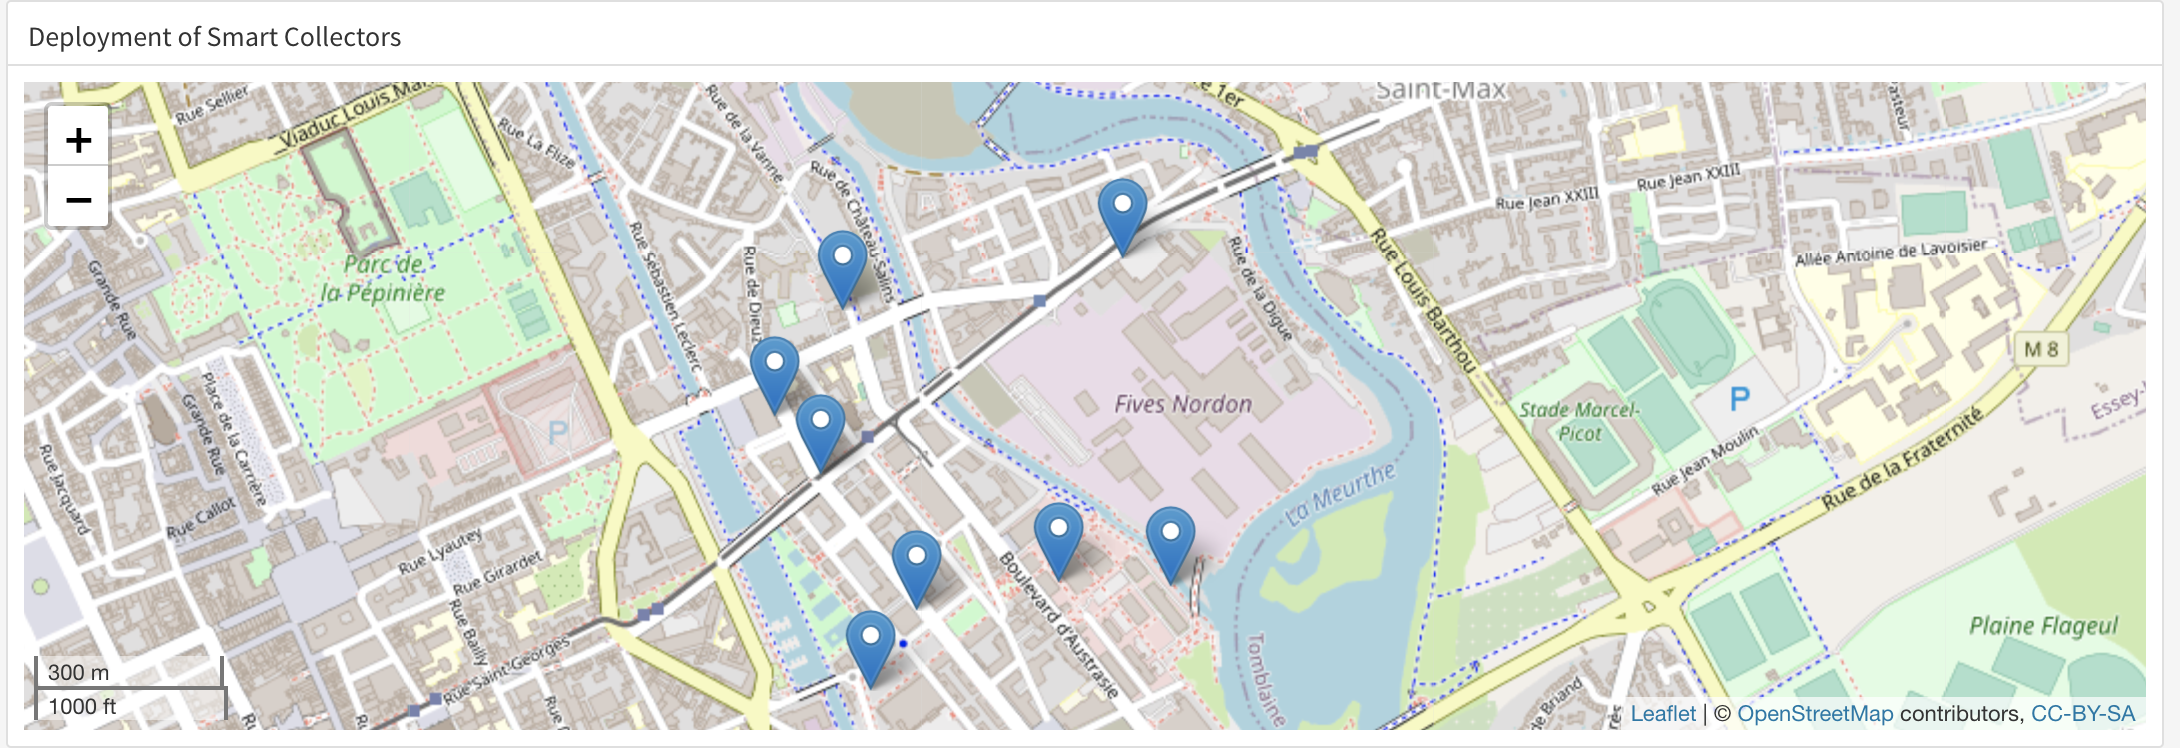
\includegraphics{figures/SC/Deployment.png}

}

\caption{\label{fig-sc-deployment}Deployment of the Smart Collectors.}

\end{figure}

The selection of the places were based on the steps 3. For the
experimentation, 8 sites were selected for the deployment as listed in
the Table~\ref{tbl-deployment}.

\hypertarget{tbl-deployment}{}
\begin{table}[H]
\caption{\label{tbl-deployment}Selected points of deployment of the smart collector in the
neighboorhood of Rives de Meurthe, Nancy - France. }\tabularnewline

\centering\begingroup\fontsize{10}{12}\selectfont

\begin{tabular}[t]{r>{\raggedright\arraybackslash}p{3cm}l>{\raggedright\arraybackslash}p{2cm}>{\raggedright\arraybackslash}p{4cm}}
\toprule
ID &  Name & Type​  & Potential public​  & Main activity\\
\midrule
\cellcolor{gray!6}{1} & \cellcolor{gray!6}{MCJ Bazin ​ } & \cellcolor{gray!6}{Association​ } & \cellcolor{gray!6}{+300​ } & \cellcolor{gray!6}{Activités culturelles/loisirs​ }\\
2 & Octroi​  & Association ​  & +1000​  & Tiers lieu, accueil de porteurs de projets et espaces de coworking​ \\
\cellcolor{gray!6}{3} & \cellcolor{gray!6}{Curves​ } & \cellcolor{gray!6}{Private Entreprise​ } & \cellcolor{gray!6}{+100​ } & \cellcolor{gray!6}{Salle de sport​ }\\
4 & ENSGSI​  & University  & 300​  & Ecole d’ingénieurs - Enseignement supérieur et recherche​ \\
\cellcolor{gray!6}{5} & \cellcolor{gray!6}{MAIF (bat.1)​ } & \cellcolor{gray!6}{Private Enterprise} & \cellcolor{gray!6}{50​ } & \cellcolor{gray!6}{Assurance mutuelle​ }\\
\addlinespace
6 & EEIGM​  & University  & 500​  & Ecole d'ingénieurs - Formation et enseignement d'ingénieurs en Génie des Matériaux ​ \\
\cellcolor{gray!6}{7} & \cellcolor{gray!6}{Voie Navigable de France​ } & \cellcolor{gray!6}{Public Entreprise​ } & \cellcolor{gray!6}{50​ } & \cellcolor{gray!6}{Gestion du réseau des voies navigables de France​ }\\
8 & Sport Nautique de Nancy​  & Association​  & +100​  & Club de sport (aviron )​ \\
\bottomrule
\end{tabular}
\endgroup{}
\end{table}

First, face-to-face meetings with the local actors were made to obtain
the agreement for the installation of the prototype. As a relevant
criteria, the installation needed to be in a location were the
visitors/employees/customers of the selected point are able to see the
device. We designed an appropriate communication that enables to explain
the purpose of the device and connect to the information of INEDIT
projet (see Figure~\ref{fig-smart})

\begin{figure}

\begin{minipage}[t]{0.62\linewidth}

{\centering 

\raisebox{-\height}{

\includegraphics[width=2.5in,height=\textheight]{figures/SC/curves.jpeg}

}

}

\subcaption{\label{fig-sc-curves}Picture of the Smart collector at the
collection point}
\end{minipage}%
%
\begin{minipage}[t]{0.38\linewidth}

{\centering 

\raisebox{-\height}{

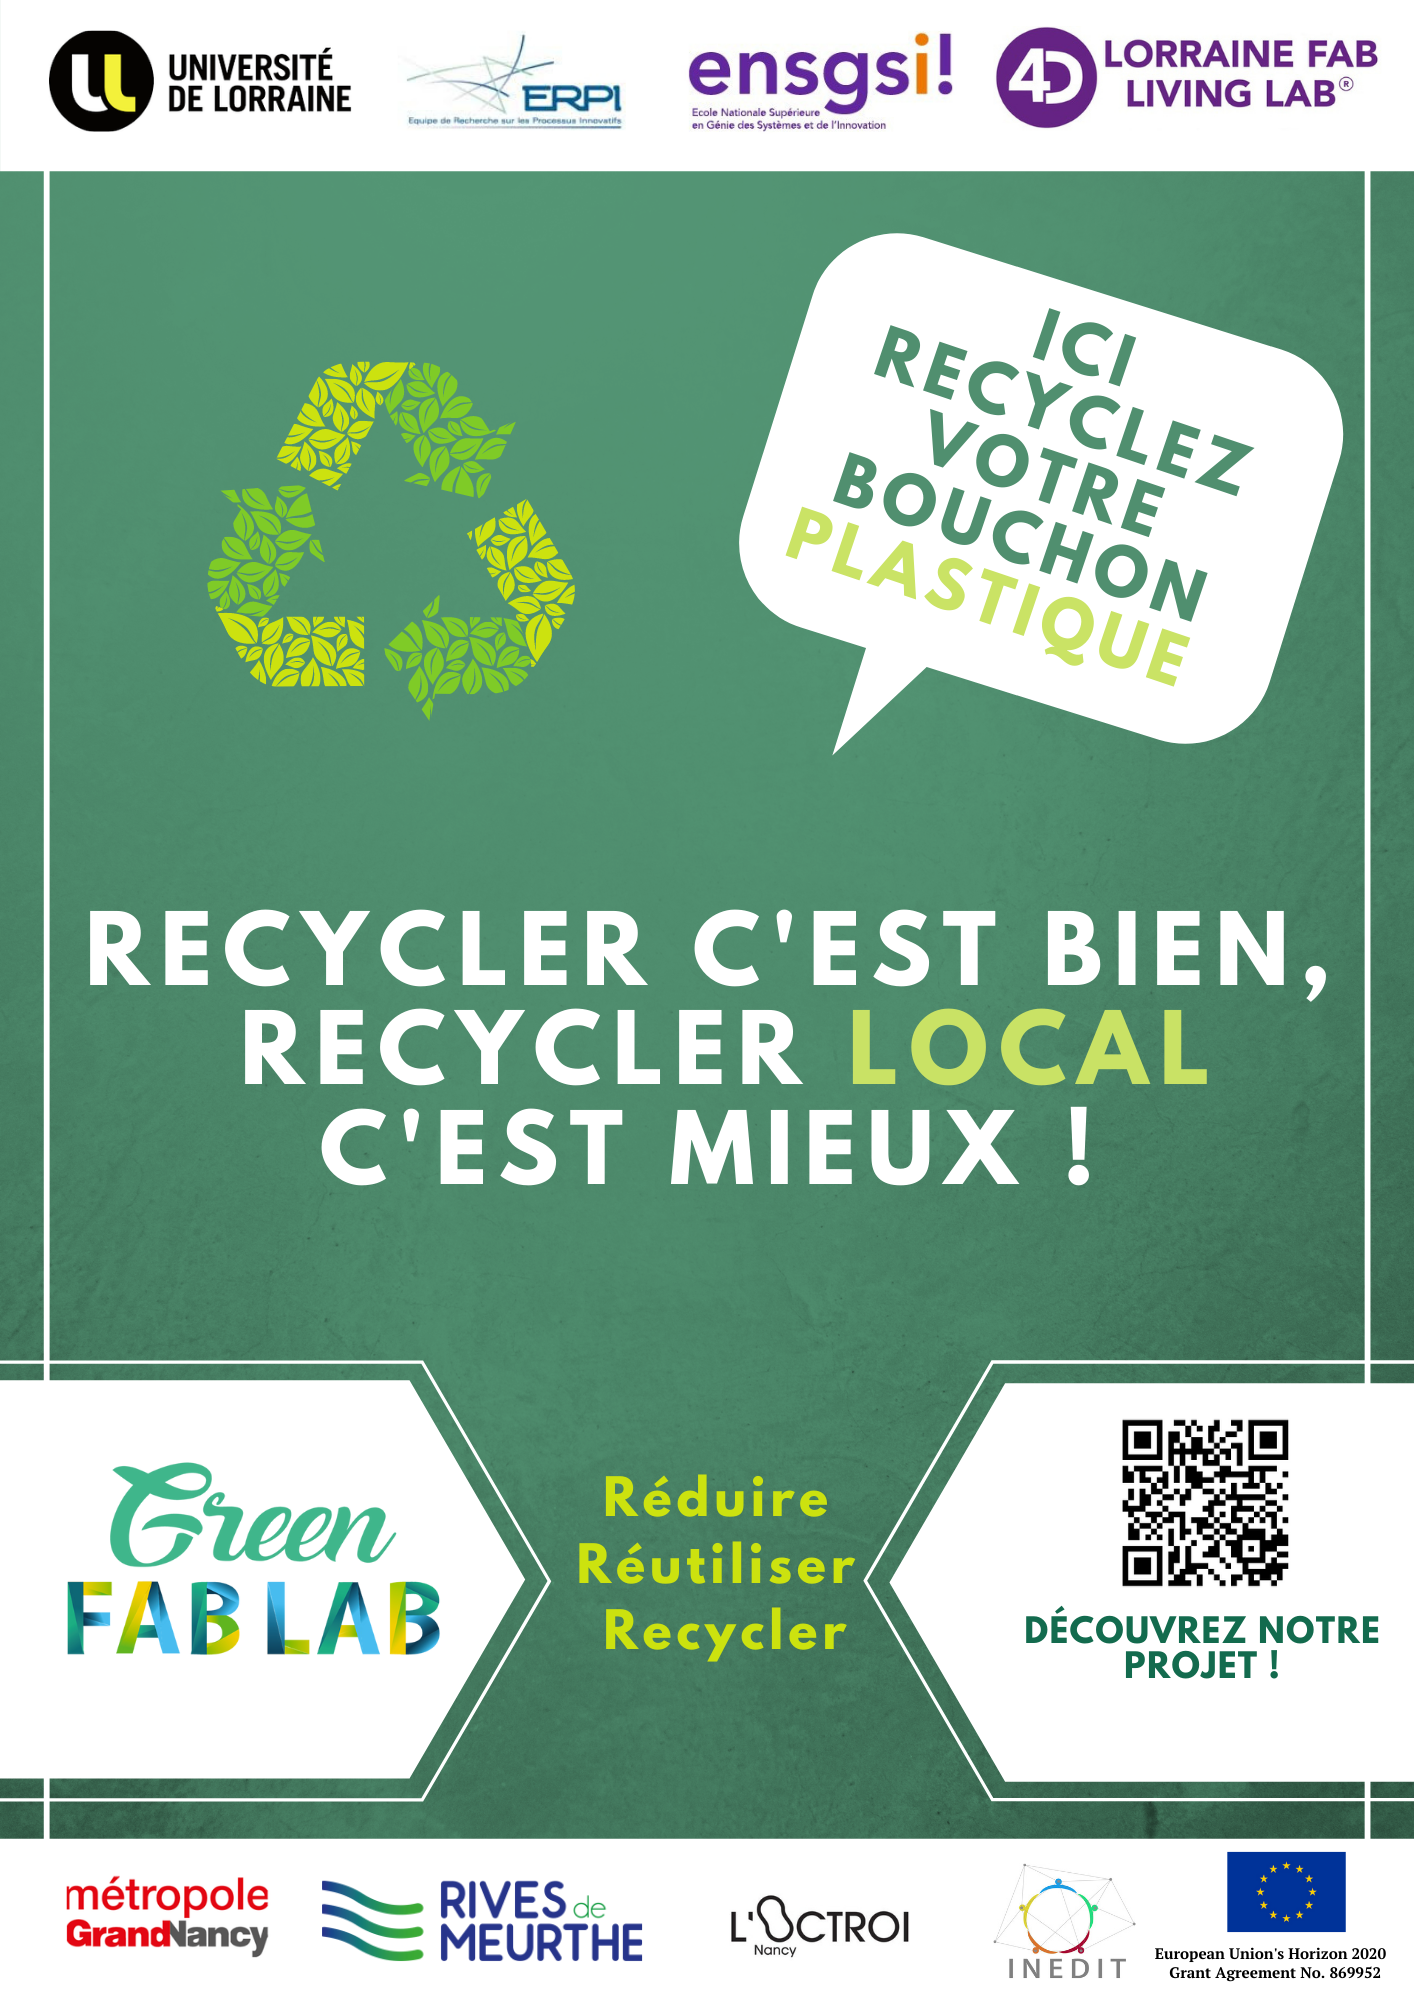
\includegraphics[width=1.5in,height=\textheight]{figures/SC/comm.png}

}

}

\subcaption{\label{fig-sc-flyer}Communication strategy of the smart
collector}
\end{minipage}%

\caption{\label{fig-smart}Smart collector}

\end{figure}

Then, a system activation is putted in place to begin the collection
gate. Once the smart collector is online, it is necessary to survey the
online dashboard to control the waste plastic quantity. In the moment
that the dashboard present a weight more than 3 kg, we mapped the
collection point in the stage of \emph{`to collect'} and we plan the
recovery. The distance of the collection place is less than \(2~km\) so
is carried out by bicycle or on foot to avoid the possible impact
produced for a combustion or electric vehicle. Once the recovery process
is made, at the Green Fablab When the waste plastic is collected, it is
stored at the facilities of the Green FabaLab before posterior treatment
and adequation.\\
we have build a central collector where the material is stored before it
is treated.

\begin{figure}[H]

{\centering 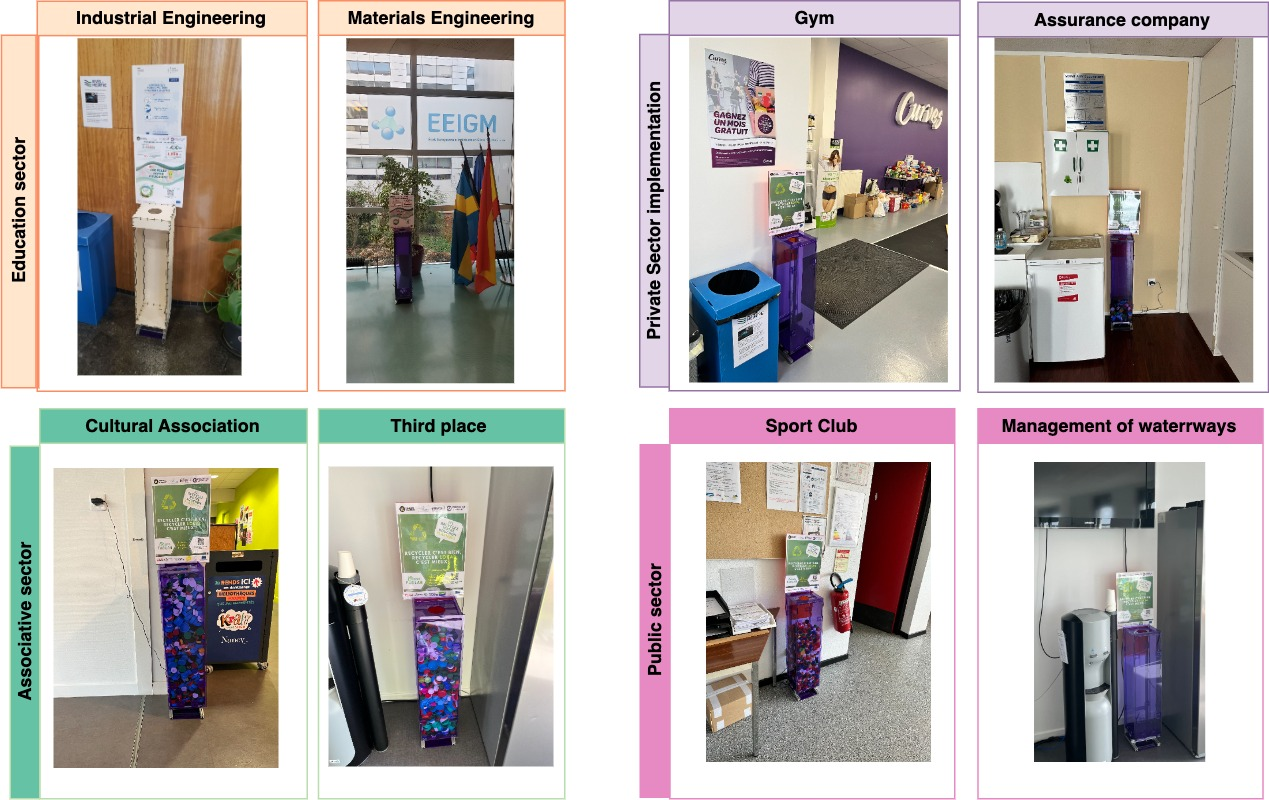
\includegraphics[width=1\textwidth,height=\textheight]{figures/SC/Smart-Collectors.pdf}

}

\caption{\label{fig-sc-flyer}Smart collectors deployed in the territory}

\end{figure}

\hypertarget{step-5-transport-waste-material-to-the-recycling-facilities}{%
\subsection{Step 5: Transport waste material to the recycling
facilities}\label{step-5-transport-waste-material-to-the-recycling-facilities}}

The recovery process took place once a week on average. The plastic
waste is collected and transported to Green Fablab facilities, and then
it is stored in a central collector as illustrated by the figure
Figure~\ref{fig-sc-recovery}.

\begin{figure}

\begin{minipage}[t]{0.50\linewidth}

{\centering 

\raisebox{-\height}{

\includegraphics[width=2in,height=\textheight]{figures/SC/Collector-bouchons-00.jpeg}

}

}

\subcaption{\label{fig-sc-collector-00}Centrla collector of plastic
waste}
\end{minipage}%
%
\begin{minipage}[t]{0.50\linewidth}

{\centering 

\raisebox{-\height}{

\includegraphics[width=2in,height=\textheight]{figures/SC/Collector-bouchons-01.jpeg}

}

}

\subcaption{\label{fig-sc-collector-01}Communication flyer for the smart
collector}
\end{minipage}%

\caption{\label{fig-sc-collector}Smart collector}

\end{figure}

Throughout the experimentation of the deployment, we have mapped the
quantity of collected material. Figure~\ref{fig-sc-recovery} corresponds
to the profile of quantity collection per month. In average, we have
collected XX\textasciitilde kg per month.

\begin{figure}[H]

{\centering 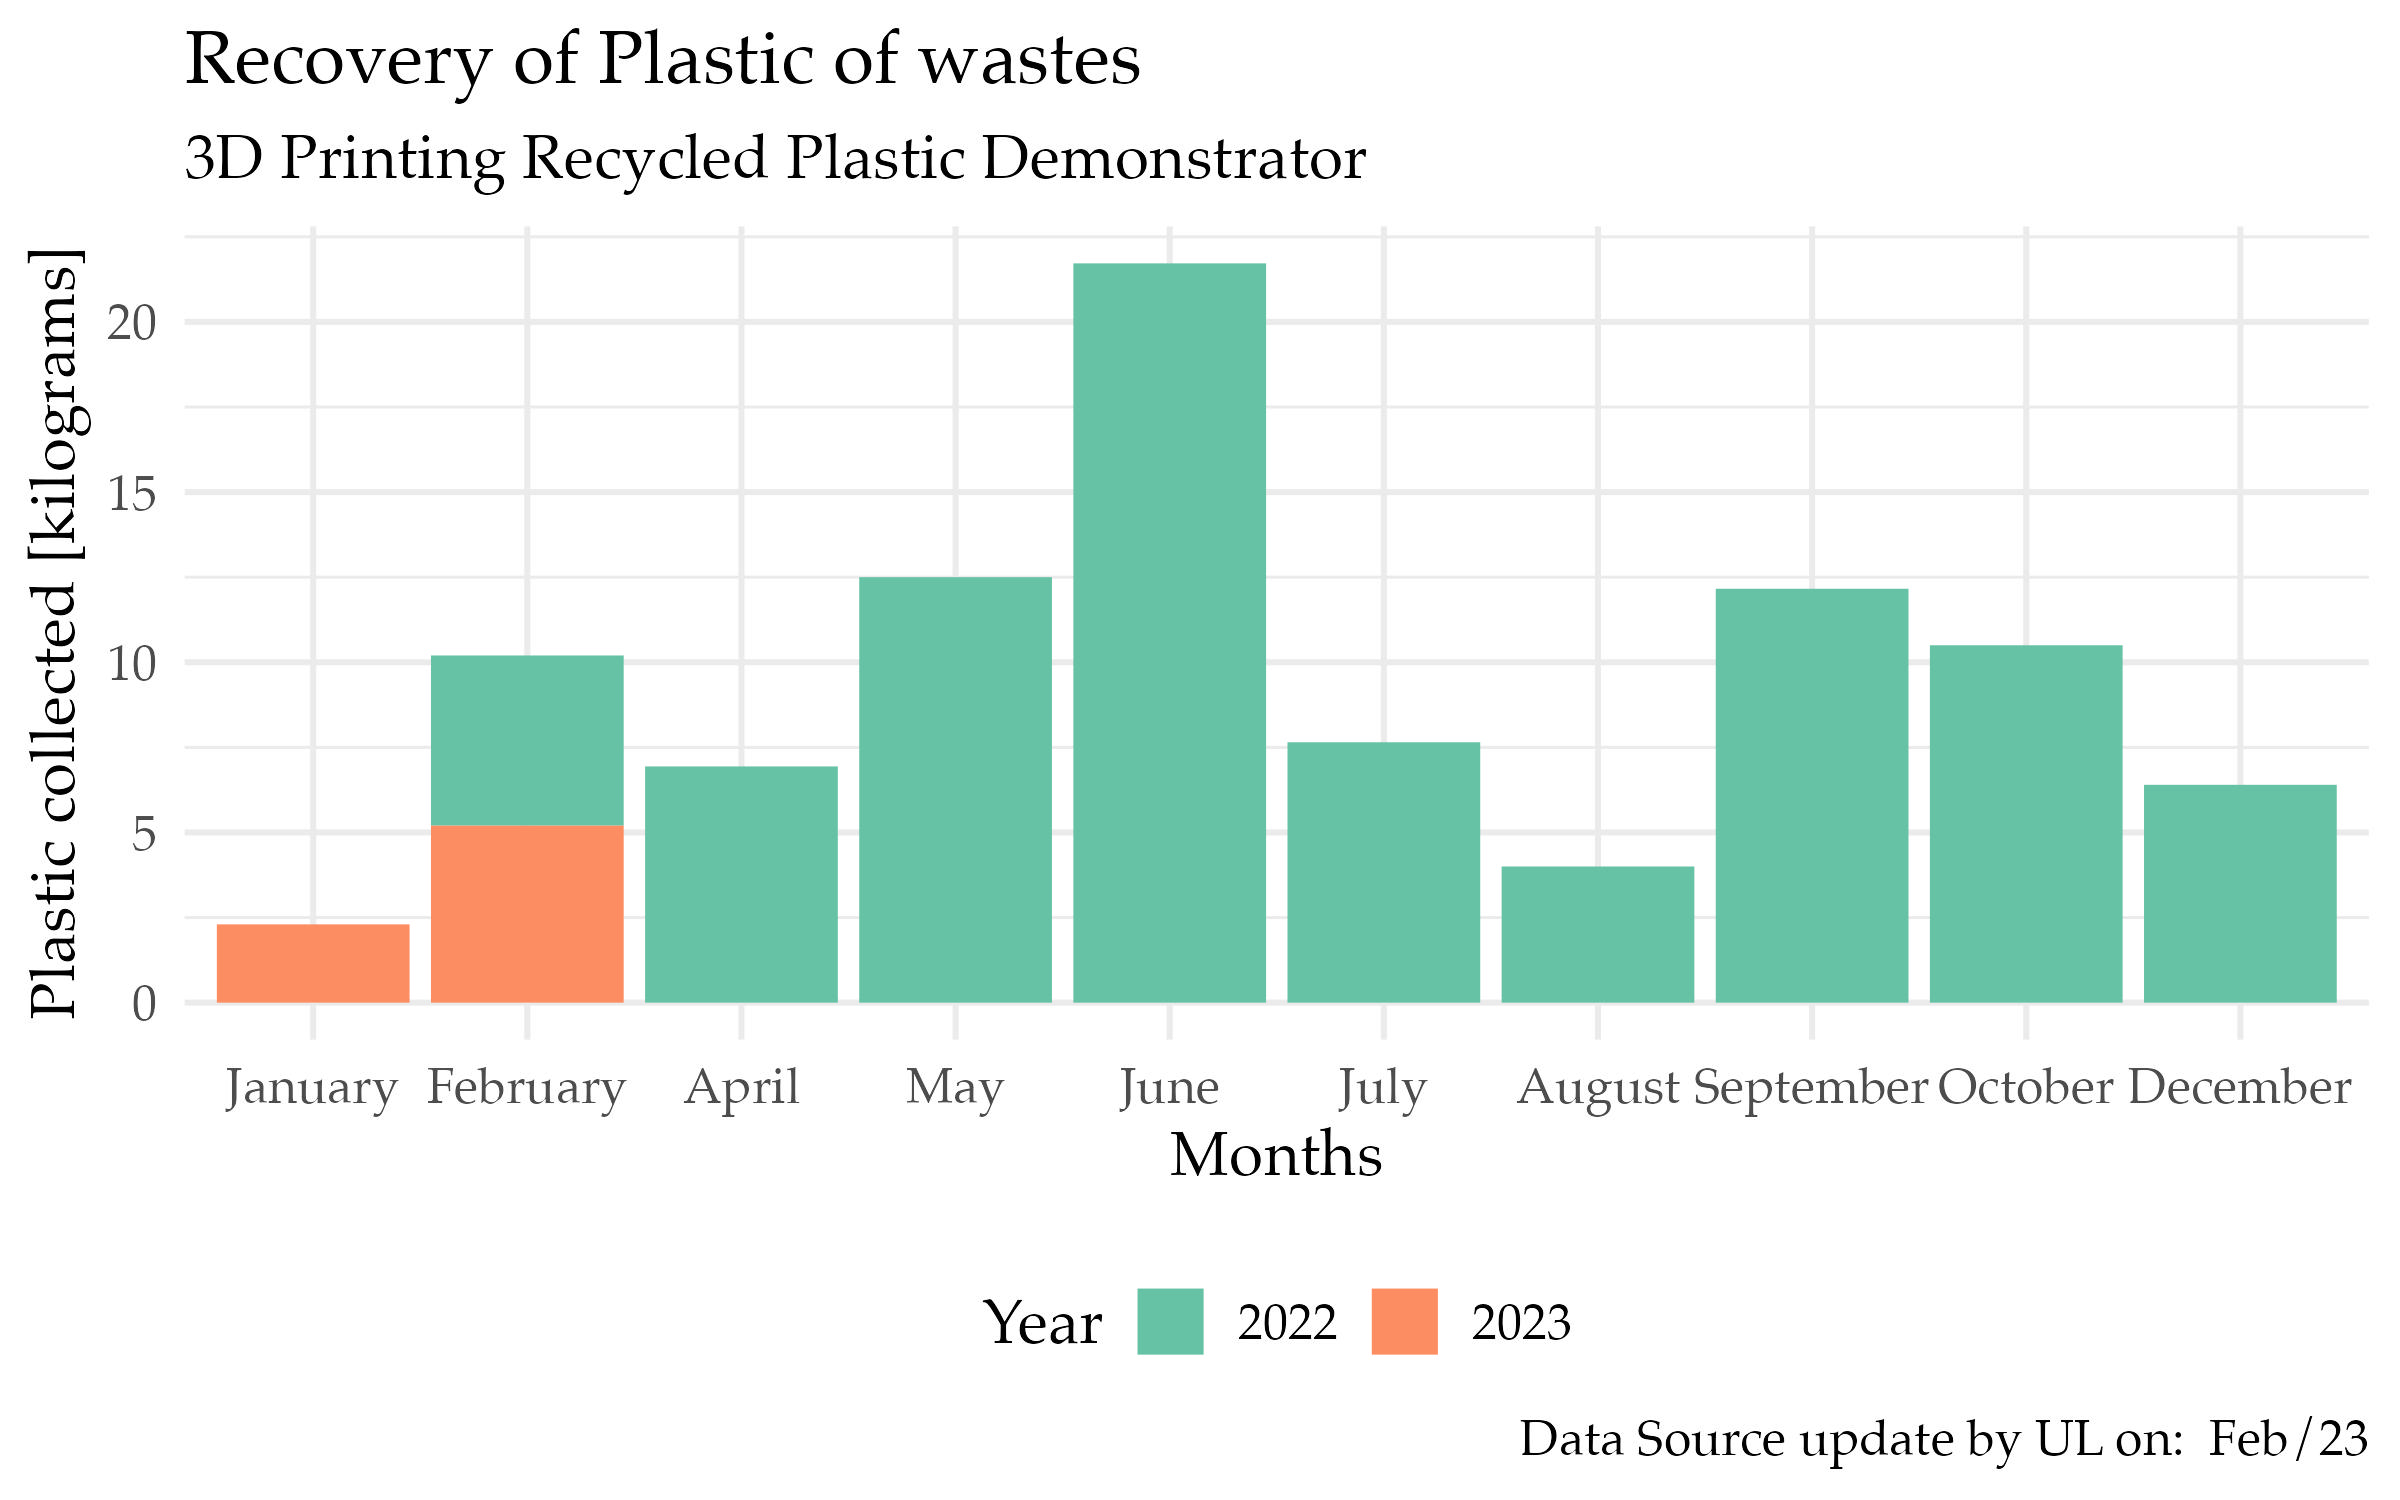
\includegraphics[width=0.9\textwidth,height=\textheight]{figures/SC/Recovery.jpg}

}

\caption{\label{fig-sc-recovery}Recovery profile of plastic}

\end{figure}

\begin{tcolorbox}[enhanced jigsaw, opacityback=0, rightrule=.15mm, leftrule=.75mm, colframe=quarto-callout-note-color-frame, breakable, toprule=.15mm, bottomtitle=1mm, left=2mm, colback=white, title=\textcolor{quarto-callout-note-color}{\faInfo}\hspace{0.5em}{Key Performance Indicator of the Recovery process}, coltitle=black, colbacktitle=quarto-callout-note-color!10!white, toptitle=1mm, arc=.35mm, bottomrule=.15mm, opacitybacktitle=0.6, titlerule=0mm]

In terms of \emph{KPI} of the recovery, from February 2022 to February
2023, we have collected a total of \(94.37~kg\) of plastic waste using 8
collectors in the territory of Rives de Meurthe, Nancy-France.

\end{tcolorbox}

\hypertarget{step-6-adequation-and-preparation-of-the-material}{%
\subsection{Step 6: Adequation and preparation of the
material}\label{step-6-adequation-and-preparation-of-the-material}}

This is the first stage carried out inside the Green FabLab. This stage
is the set of activities required for the plastic waste to be adapted
for further use. The Green FabLab works mainly with 4 types of plastic
at the moment. The most common are high density polyethylene (HDPE) and
polypropylene (PP), which are the main plastics used in the production
of bottle caps and they are collected in the smart collector. The
plastic waste from unused/damaged 3D printing parts are mainly of
polylactic acid (PLA) are collected from mainly from the Lorraine Fab
Living Lab. And finally, the plastic bottles also are collected which
are polyethylene terephthalate (PET).

The preparation process begins with the separation and identification of
each plastic collected. As already mentioned, the plastics used in the
Green FabLab are 4 (HDPE, PP, PET and PLA) and are separated by type of
plastic and colour. This process is carried out manually.

\begin{figure}[H]

{\centering 
\includegraphics[width=0.5\textwidth,height=\textheight]{figures/Image-to-add.png}

}

\caption{Photo of the sorting process}

\end{figure}

The second step is the cleaning phase. Cleaning and washing plastic cups
and bottles is crucial step for effective recycling because plastics are
mainly post-consumer waste, they are not in an adequate state of
cleanliness. It is required that to ensure the plastic is as clean as
possible because dirty material can affect the quality of the extrusion
/ printing process, which at the end affects the recycled product.
Therefore, we aims to remove adhesives, leftover waste, and labels. HDPE
and PP are mainly used in the plastic injection molding process, while
PLA and PET (Mixed with 9\% HDPE) are used in 3D printing.

\begin{figure}[H]

{\centering 
\includegraphics[width=0.5\textwidth,height=\textheight]{figures/Image-to-add.png}

}

\caption{Photo of the cleaning process}

\end{figure}

In a first moment, the manual cleaning is used in the Green Fablab to
remove the most of the majors contaminant present in the material. For
plastic injection moulding, where mainly PP and HDPE are used, the
plastic is washed in a sink with hot water.\\
The water consumption per gram is approximately \(4L/1000g\). The drying
of the plastic is done by natural convection in the open air.

For additive manufacturing, where mainly PLA, HDPE and PET blends are
used, the cleaning process is much more controlled. The process is
carried out in a small ultrasonic cleaning machine, to ensure that
impurities are removed. The cleaner ultrasonic machine wash 200gr de
plástico en 1 L of water. This process takes 20 mins with a consuption
of 2kWh.

\begin{figure}[H]

{\centering 
\includegraphics[width=5.20833in,height=\textheight]{figures/Image-to-add.png}

}

\caption{Photo of the Ultrasonic cleaning}

\end{figure}

The second step in the preparation of the waste material is the size
reduction process. In this step, the washed and sorted plastic is sent
through shredding machine where it is grounded into smaller pieces of
plastic. A critical parameters in the control of the granulometry. The
purpose of the size reduction is to obtain plastic waste where the
granulometry correspond to the extrusion / printing. The plastic waste
need to be in reduced from a range of between 25-50 mm to 3-5mm
approximately after grinding. A cutting mill machine SM 300
Retsch\textsuperscript{\textregistered} with a selectable speed range
from 700 to 3,000 \(rpm\) was used. The selected speed was \(1500~rpm\).
Normally we use a rotational speed of 1500 which produces an energy
consumption of 0.7 kWh. The process takes 15 minutes per kilogram of
material with a loss of approximately 10\%. For direct additive
manufacturing the optimum size for the granulometry for printing is
between 3 and 5mm. Therefore, after shredding it is necessary to
sieve.\\
In terms of plastic injection moulding, the plastic flakes can be
slightly larger than those required for 3D printing.

\begin{figure}[H]

{\centering 
\includegraphics[width=5.20833in,height=\textheight]{figures/Image-to-add.png}

}

\caption{Photo of the Shredding process}

\end{figure}

Filament is produced at 0.4 kg/h using 0.24 kWh/kg with a diameter
±4.6\%. 3Devo

To remove all the moisture from the plastic it is necessary to carry out
a drying process in a conventional oven.\\
In the drying phase, the plastic is putted in the oven at 60°C during
15h with a consumption of 0,061 Kwh.

Finally, the drying process is last step to prepare the material.

\hypertarget{step-7-path-planning---3d-printing}{%
\subsection{Step 7: Path planning - 3D
Printing}\label{step-7-path-planning---3d-printing}}

Once, we have the model to concerning the

\begin{figure}[H]

{\centering 
\includegraphics[width=5.20833in,height=\textheight]{figures/Image-to-add.png}

}

\caption{Photo of the Slicer of the Gigzbot}

\end{figure}

\hypertarget{step-8-post-processing}{%
\subsection{Step 8 : Post-processing}\label{step-8-post-processing}}

Post-processing relies to the treatment of the injected and/or printed
part. Regarding the injection part, the post-processing relies in the

Concerning the 3D printing part, one of the most

\hypertarget{step-9-implementation-examples}{%
\subsection{Step 9: Implementation
Examples}\label{step-9-implementation-examples}}

\hypertarget{case-workbech-1}{%
\subsubsection{Case Workbech 1}\label{case-workbech-1}}

This user case aims the validation of the for personalization of the

\begin{figure}[H]

{\centering 
\includegraphics[width=5.20833in,height=\textheight]{figures/Image-to-add.png}

}

\caption{Photo of the Slicer of the Gigzbot}

\end{figure}

\hypertarget{case-workbech-1-1}{%
\subsubsection{Case Workbech 1}\label{case-workbech-1-1}}

\begin{figure}[H]

{\centering 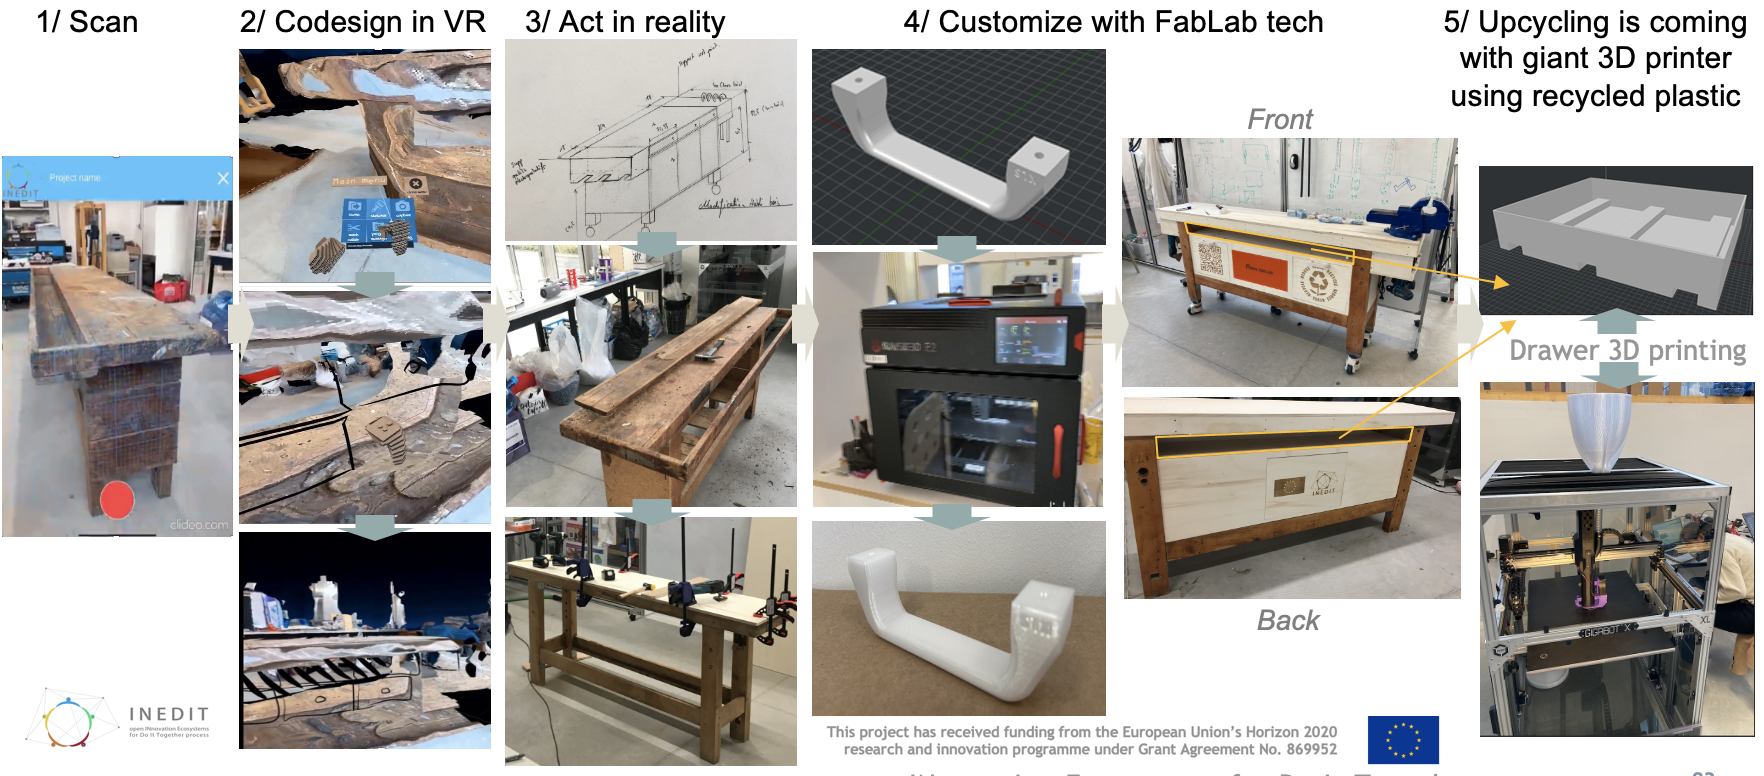
\includegraphics[width=0.9\textwidth,height=\textheight]{figures/demos/workbench/2022-02-24 Processus INEDIT.png}

}

\caption{Photo of the Slicer of the Gigzbot}

\end{figure}

\hypertarget{step-10-re-design-and-improvements-of-fabrication}{%
\subsection{Step 10: Re-design and improvements of
fabrication}\label{step-10-re-design-and-improvements-of-fabrication}}

\hypertarget{step-11-validation}{%
\subsection{Step 11: Validation}\label{step-11-validation}}

\newpage

\hypertarget{conclusions}{%
\section{Conclusions}\label{conclusions}}

Plastic waste as secondary ressources and possibilities for a secondary
market

Qualification of the waste

Mains challenges to tackle

Legislation of waste and

More examples neeed it in the recycling for education purposes

\newpage

\hypertarget{bibliography}{%
\section*{Bibliography}\label{bibliography}}
\addcontentsline{toc}{section}{Bibliography}

\hypertarget{refs}{}
\begin{CSLReferences}{1}{0}
\leavevmode\vadjust pre{\hypertarget{ref-Anderson2017}{}}%
Anderson, I., 2017. Mechanical {Properties} of {Specimens 3D Printed}
with {Virgin} and {Recycled Polylactic Acid}. 3D Printing and Additive
Manufacturing 4, 110--115. \url{https://doi.org/10.1089/3dp.2016.0054}

\leavevmode\vadjust pre{\hypertarget{ref-Bano2020}{}}%
Bano, A., Ud Din, I., Al-Huqail, A.A., 2020. {AIoT-Based Smart Bin} for
{Real-Time Monitoring} and {Management} of {Solid Waste}. Scientific
Programming 2020. \url{https://doi.org/10.1155/2020/6613263}

\leavevmode\vadjust pre{\hypertarget{ref-Beltagui2020}{}}%
Beltagui, A., Sesis, A., Stylos, N., 2021. A bricolage perspective on
democratising innovation: {The} case of {3D} printing in makerspaces.
Technological Forecasting and Social Change 163, 120453.
\url{https://doi.org/10.1016/j.techfore.2020.120453}

\leavevmode\vadjust pre{\hypertarget{ref-Birtchnell2013a}{}}%
Birtchnell, T., Urry, J., 2013. Fabricating {Futures} and the {Movement}
of {Objects}. Mobilities 8, 388--405.
\url{https://doi.org/10.1080/17450101.2012.745697}

\leavevmode\vadjust pre{\hypertarget{ref-BonninRoca2019}{}}%
Bonnín Roca, J., Vaishnav, P., Laureijs, R.E., Mendonça, J., Fuchs,
E.R.H., 2019. Technology cost drivers for a potential transition to
decentralized manufacturing. Additive Manufacturing 28, 136--151.
\url{https://doi.org/10.1016/j.addma.2019.04.010}

\leavevmode\vadjust pre{\hypertarget{ref-Boujut2003}{}}%
Boujut, J.-F., Blanco, E., 2003. Intermediary {Objects} as a mean to
foster {Co-operation}. Engineering Design Computer Supported Cooperative
Work 205--219.

\leavevmode\vadjust pre{\hypertarget{ref-Bourell2017}{}}%
Bourell, D., Kruth, J.P., Leu, M., Levy, G., Rosen, D., Beese, A.M.,
Clare, A., 2017. Materials for additive manufacturing. CIRP Annals 66,
659--681. \url{https://doi.org/10.1016/j.cirp.2017.05.009}

\leavevmode\vadjust pre{\hypertarget{ref-Brenken2017}{}}%
Brenken, B., Barocio, E., Favaloro, A., Kunc, V., Pipes, R.B., 2018.
Fused filament fabrication of fiber-reinforced polymers: {A} review.
Additive Manufacturing 21, 1--16.
\url{https://doi.org/10.1016/j.addma.2018.01.002}

\leavevmode\vadjust pre{\hypertarget{ref-Canessa2017}{}}%
Canessa, E., Baruzzo, M., Fonda, C., 2017. Study of {Moineau-based}
pumps for the volumetric extrusion of pellets. Additive Manufacturing
17, 143--150. \url{https://doi.org/10.1016/j.addma.2017.08.015}

\leavevmode\vadjust pre{\hypertarget{ref-Catania2014}{}}%
Catania, V., Ventura, D., 2014. An approch for monitoring and smart
planning of urban solid waste management using smart-{M3} platform, in:
Conference of {Open Innovation Association}, {FRUCT}. {IEEE Computer
Society}, pp. 24--31. \url{https://doi.org/10.1109/FRUCT.2014.6872422}

\leavevmode\vadjust pre{\hypertarget{ref-Chen2017}{}}%
Chen, L., He, Y., Yang, Y., Niu, S., Ren, H., 2017. The research status
and development trend of additive manufacturing technology. The
International Journal of Advanced Manufacturing Technology 89,
3651--3660. \url{https://doi.org/10.1007/s00170-016-9335-4}

\leavevmode\vadjust pre{\hypertarget{ref-CruzSanchez2020}{}}%
Cruz Sanchez, F.A., Boudaoud, H., Camargo, M., Pearce, J.M., 2020.
Plastic recycling in additive manufacturing: {A} systematic literature
review and opportunities for the circular economy. Journal of Cleaner
Production 264, 121602.
\url{https://doi.org/10.1016/j.jclepro.2020.121602}

\leavevmode\vadjust pre{\hypertarget{ref-CruzSanchez2017}{}}%
Cruz Sanchez, F.A., Boudaoud, H., Hoppe, S., Camargo, M., 2017. Polymer
recycling in an open-source additive manufacturing context: {Mechanical}
issues. Additive Manufacturing 17, 87--105.
\url{https://doi.org/10.1016/j.addma.2017.05.013}

\leavevmode\vadjust pre{\hypertarget{ref-ReportsAndData2019}{}}%
Data, R.A., 2019. {ReportsAndData2019}. Additive Manufacturing Market To
Reach USD 23.33 Billion By 2026.

\leavevmode\vadjust pre{\hypertarget{ref-Despeisse2016}{}}%
Despeisse, M., Baumers, M., Brown, P., Charnley, F., Ford, S.J.,
Garmulewicz, A., Knowles, S., Minshall, T.H.W., Mortara, L.,
Reed-Tsochas, F.P., Rowley, J., 2017. Unlocking value for a circular
economy through {3D} printing: {A} research agenda. Technological
Forecasting and Social Change 115, 75--84.
\url{https://doi.org/10.1016/j.techfore.2016.09.021}

\leavevmode\vadjust pre{\hypertarget{ref-Dupont2014}{}}%
Dupont, L., Morel, L., Hubert, J., Guidat, C., 2014. Study case: {Living
Lab Mode} for urban project design: {Emergence} of an ad hoc methodology
through collaborative innovation, in: 2014 {International Conference} on
{Engineering}, {Technology} and {Innovation} ({ICE}). {IEEE}, {Bergamo},
pp. 1--9. \url{https://doi.org/10.1109/ICE.2014.6871550}

\leavevmode\vadjust pre{\hypertarget{ref-Dupont2015b}{}}%
Dupont, L., Morel, L., Lhoste, P., 2015. L ' innovation {Médiation}
scientifique , territorialité et développement local. Actes des Journées
Hubert Curien, session Médiation Scientifique, territorialité et
développement local, Colloque Science \& You 2--8.

\leavevmode\vadjust pre{\hypertarget{ref-Dupont2016}{}}%
Dupont, L., Pallot, M., Morel, L., Pallot, M., 2016. Exploring the
{Appropriateness} of {Different Immersive Environments} in the {Context}
of an {Innovation Process} for {Smart Cities}. 22nd ICE/IEEE
International Technology Management Conference, 13--15.

\leavevmode\vadjust pre{\hypertarget{ref-EC2018}{}}%
European Commission, 2018. A european strategy for plastics in a
circular economy, COM (2018). {European Commission}, {Brussels}.
\url{https://doi.org/10.1021/acs.est.7b02368}

\leavevmode\vadjust pre{\hypertarget{ref-fatimah2020}{}}%
Fatimah, Y.A., Govindan, K., Murniningsih, R., Setiawan, A., 2020.
Industry 4.0 based sustainable circular economy approach for smart waste
management system to achieve sustainable development goals: {A} case
study of {Indonesia}. Journal of Cleaner Production 269, 122263.
\url{https://doi.org/10.1016/j.jclepro.2020.122263}

\leavevmode\vadjust pre{\hypertarget{ref-gabriel2023}{}}%
Gabriel, A., Cruz, F., 2023. Open source {IoT-based} collection bin
applied to local plastic recycling. HardwareX 13, e00389.
\url{https://doi.org/10.1016/j.ohx.2022.e00389}

\leavevmode\vadjust pre{\hypertarget{ref-Geissdoerfer2017}{}}%
Geissdoerfer, M., Savaget, P., Bocken, N.M.P., Hultink, E.J., 2017. The
{Circular Economy} \textendash{} {A} new sustainability paradigm?
Journal of Cleaner Production 143, 757--768.
\url{https://doi.org/10.1016/j.jclepro.2016.12.048}

\leavevmode\vadjust pre{\hypertarget{ref-Mueller2012}{}}%
Gibson, I., Rosen, D.W., Stucker, B., 2010. Additive {Manufacturing
Technologies}, Assembly Automation. {Springer US}, {Boston, MA}.
\url{https://doi.org/10.1007/978-1-4419-1120-9}

\leavevmode\vadjust pre{\hypertarget{ref-Hahladakis2018}{}}%
Hahladakis, J.N., Iacovidou, E., 2018. Closing the loop on plastic
packaging materials: {What} is quality and how does it affect their
circularity? Science of The Total Environment 630, 1394--1400.
\url{https://doi.org/10.1016/j.scitotenv.2018.02.330}

\leavevmode\vadjust pre{\hypertarget{ref-Hart2018}{}}%
Hart, K.R., Frketic, J.B., Brown, J.R., 2018. Recycling
meal-ready-to-eat ({MRE}) pouches into polymer filament for material
extrusion additive manufacturing. Additive Manufacturing 21, 536--543.
\url{https://doi.org/10.1016/j.addma.2018.04.011}

\leavevmode\vadjust pre{\hypertarget{ref-Hienerth2014}{}}%
Hienerth, C., von Hippel, E., Berg Jensen, M., 2014. User community vs.
Producer innovation development efficiency: {A} first empirical study.
Research Policy 43, 190--201.
\url{https://doi.org/10.1016/j.respol.2013.07.010}

\leavevmode\vadjust pre{\hypertarget{ref-Hofstatter2017}{}}%
Hofstätter, T., Pedersen, D.B., Tosello, G., Hansen, H.N., 2017.
State-of-the-art of fiber-reinforced polymers in additive manufacturing
technologies. Journal of Reinforced Plastics and Composites 36,
1061--1073. \url{https://doi.org/10.1177/0731684417695648}

\leavevmode\vadjust pre{\hypertarget{ref-Holmstrom2016}{}}%
Holmström, J., Holweg, M., Khajavi, S.H., Partanen, J., 2016. The direct
digital manufacturing (r)evolution: Definition of a research agenda.
Operations Management Research 9, 1--10.
\url{https://doi.org/10.1007/s12063-016-0106-z}

\leavevmode\vadjust pre{\hypertarget{ref-Hopewell2009}{}}%
Hopewell, J., Dvorak, R., Kosior, E., 2009. Plastics recycling:
Challenges and opportunities. Philosophical Transactions of the Royal
Society B: Biological Sciences 364, 2115--2126.
\url{https://doi.org/10.1098/rstb.2008.0311}

\leavevmode\vadjust pre{\hypertarget{ref-Jiang2017}{}}%
Jiang, R., Kleer, R., Piller, F.T., 2017. Predicting the future of
additive manufacturing: {A Delphi} study on economic and societal
implications of {3D} printing for 2030. Technological Forecasting and
Social Change 117, 84--97.
\url{https://doi.org/10.1016/j.techfore.2017.01.006}

\leavevmode\vadjust pre{\hypertarget{ref-Karaylan2021}{}}%
Karayılan, S., Yılmaz, Ö., Uysal, Ç., Naneci, S., 2021. Prospective
evaluation of circular economy practices within plastic packaging value
chain through optimization of life cycle impacts and circularity.
Resources, Conservation and Recycling 173, 105691.
\url{https://doi.org/10.1016/j.resconrec.2021.105691}

\leavevmode\vadjust pre{\hypertarget{ref-Kranzinger2018}{}}%
Kranzinger, L., Pomberger, R., Schwabl, D., Flachberger, H., Bauer, M.,
Lehner, M., Hofer, W., 2018. Output-oriented analysis of the wet
mechanical processing of polyolefin-rich waste for feedstock recycling.
Waste Management \& Research 36, 445--453.
\url{https://doi.org/10.1177/0734242X18764294}

\leavevmode\vadjust pre{\hypertarget{ref-Kreiger2013}{}}%
Kreiger, M., Pearce, J.M., 2013. Environmental {Impacts} of {Distributed
Manufacturing} from 3-{D Printing} of {Polymer Components} and
{Products}. MRS Proceedings 1492, 85--90.
\url{https://doi.org/10.1557/opl.2013.319}

\leavevmode\vadjust pre{\hypertarget{ref-Kucherov2017}{}}%
Kucherov, F.A., Gordeev, E.G., Kashin, A.S., Ananikov, V.P., 2017.
Three-{Dimensional Printing} with {Biomass-Derived PEF} for
{Carbon-Neutral Manufacturing}. Angewandte Chemie International Edition
56, 15931--15935. \url{https://doi.org/10.1002/anie.201708528}

\leavevmode\vadjust pre{\hypertarget{ref-Laplume2016}{}}%
Laplume, A.O., Petersen, B., Pearce, J.M., 2016. Global value chains
from a {3D} printing perspective. Journal of International Business
Studies 47, 595--609. \url{https://doi.org/10.1057/jibs.2015.47}

\leavevmode\vadjust pre{\hypertarget{ref-Little2020}{}}%
Little, H.A., Tanikella, N.G., J. Reich, M., Fiedler, M.J., Snabes,
S.L., Pearce, J.M., 2020. Towards {Distributed Recycling} with {Additive
Manufacturing} of {PET Flake Feedstocks}. Materials 13, 4273.
\url{https://doi.org/10.3390/ma13194273}

\leavevmode\vadjust pre{\hypertarget{ref-Matt2015}{}}%
Matt, D.T., Rauch, E., Dallasega, P., 2015. Trends towards {Distributed
Manufacturing Systems} and {Modern Forms} for their {Design}. Procedia
CIRP 33, 185--190. \url{https://doi.org/10.1016/j.procir.2015.06.034}

\leavevmode\vadjust pre{\hypertarget{ref-Mohan2017}{}}%
Mohan, N., Senthil, P., Vinodh, S., Jayanth, N., 2017. A review on
composite materials and process parameters optimisation for the fused
deposition modelling process. Virtual and Physical Prototyping 12,
47--59. \url{https://doi.org/10.1080/17452759.2016.1274490}

\leavevmode\vadjust pre{\hypertarget{ref-Ngo2018}{}}%
Ngo, T.D., Kashani, A., Imbalzano, G., Nguyen, K.T.Q., Hui, D., 2018.
Additive manufacturing ({3D} printing): {A} review of materials,
methods, applications and challenges. Composites Part B: Engineering
143, 172--196. \url{https://doi.org/10.1016/j.compositesb.2018.02.012}

\leavevmode\vadjust pre{\hypertarget{ref-Niaki2019}{}}%
Niaki, M.K., Torabi, S.A., Nonino, F., 2019. Why manufacturers adopt
additive manufacturing technologies: {The} role of sustainability.
Journal of Cleaner Production 222, 381--392.
\url{https://doi.org/10.1016/j.jclepro.2019.03.019}

\leavevmode\vadjust pre{\hypertarget{ref-pallot2021}{}}%
Pallot, M., Dupont, L., Fleury, S., Araque-Tellez, G., Richir, S., 2021.
Investigating the {Impact} of {Visual Representations} during
{Ideation}: {Towards Immersive eXperience Design}, in: 2021 {IEEE
International Conference} on {Engineering}, {Technology} and
{Innovation} ({ICE}/{ITMC}). {IEEE}, p. 1.
\url{https://doi.org/10.1109/ICE/ITMC52061.2021.9570244}

\leavevmode\vadjust pre{\hypertarget{ref-Pearce2009}{}}%
Pearce, J.M., Mushtaq, U., 2009. Overcoming technical constraints for
obtaining sustainable development with open source appropriate
technology. TIC-STH'09: 2009 IEEE Toronto International Conference -
Science and Technology for Humanity 814--820.
\url{https://doi.org/10.1109/TIC-STH.2009.5444388}

\leavevmode\vadjust pre{\hypertarget{ref-Petersen2017a}{}}%
Petersen, E., Pearce, J., 2017. Emergence of {Home Manufacturing} in the
{Developed World}: {Return} on {Investment} for {Open-Source} 3-{D
Printers}. Technologies 5, 7.
\url{https://doi.org/10.3390/technologies5010007}

\leavevmode\vadjust pre{\hypertarget{ref-Petrovic2011}{}}%
Petrovic, V., Vicente Haro Gonzalez, J., Jordá Ferrando, O., Delgado
Gordillo, J., Ramón Blasco Puchades, J., Portolés Griñan, L., 2011.
Additive layered manufacturing: Sectors of industrial application shown
through case studies. International Journal of Production Research 49,
1061--1079. \url{https://doi.org/10.1080/00207540903479786}

\leavevmode\vadjust pre{\hypertarget{ref-Plastics2019}{}}%
Plastics, E., 2019. Plastics - the {Facts} 2019.

\leavevmode\vadjust pre{\hypertarget{ref-Rahman2018}{}}%
Rahman, Z., Barakh Ali, S.F., Ozkan, T., Charoo, N.A., Reddy, I.K.,
Khan, M.A., 2018. Additive {Manufacturing} with {3D Printing}:
{Progress} from {Bench} to {Bedside}. The AAPS Journal 20, 101.
\url{https://doi.org/10.1208/s12248-018-0225-6}

\leavevmode\vadjust pre{\hypertarget{ref-Ranjbari2021}{}}%
Ranjbari, M., Saidani, M., Esfandabadi, Z.S., Peng, W., Lam, S.S.,
Aghbashlo, M., Quatraro, F., Tabatabaei, M., Shams Esfandabadi, Z.,
Peng, W., Lam, S.S., Aghbashlo, M., Quatraro, F., Tabatabaei, M., 2021.
Two decades of research on waste management in the circular economy:
{Insights} from bibliometric, text mining, and content analyses. Journal
of Cleaner Production 314, 128009.
\url{https://doi.org/10.1016/j.jclepro.2021.128009}

\leavevmode\vadjust pre{\hypertarget{ref-rejeb2022}{}}%
Rejeb, A., Suhaiza, Z., Rejeb, K., Seuring, S., Treiblmaier, H., 2022.
The {Internet} of {Things} and the circular economy: {A} systematic
literature review and research agenda. Journal of Cleaner Production
350, 131439. \url{https://doi.org/10.1016/J.JCLEPRO.2022.131439}

\leavevmode\vadjust pre{\hypertarget{ref-Ryberg2019}{}}%
Ryberg, M.W., Hauschild, M.Z., Wang, F., Averous-Monnery, S., Laurent,
A., 2019. Global environmental losses of plastics across their value
chains. Resources, Conservation and Recycling 151, 104459.
\url{https://doi.org/10.1016/j.resconrec.2019.104459}

\leavevmode\vadjust pre{\hypertarget{ref-Santander2020}{}}%
Santander, P., Cruz Sanchez, F.A., Boudaoud, H., Camargo, M., 2020.
Closed loop supply chain network for local and distributed plastic
recycling for {3D} printing: A {MILP-based} optimization approach.
Resources, Conservation and Recycling 154, 104531.
\url{https://doi.org/10.1016/j.resconrec.2019.104531}

\leavevmode\vadjust pre{\hypertarget{ref-Simon2019}{}}%
Simon, B., 2019. What are the most significant aspects of supporting the
circular economy in the plastic industry? Resources, Conservation and
Recycling 141, 299--300.
\url{https://doi.org/10.1016/j.resconrec.2018.10.044}

\leavevmode\vadjust pre{\hypertarget{ref-Singh2017}{}}%
Singh, S., Ramakrishna, S., Singh, R., 2017. Material issues in additive
manufacturing: {A} review. Journal of Manufacturing Processes 25,
185--200. \url{https://doi.org/10.1016/j.jmapro.2016.11.006}

\leavevmode\vadjust pre{\hypertarget{ref-Thompson2009b}{}}%
Thompson, R.C., Moore, C.J., vom Saal, F.S., Swan, S.H., 2009. Plastics,
the environment and human health: Current consensus and future trends.
Philosophical Transactions of the Royal Society B: Biological Sciences
364, 2153--2166. \url{https://doi.org/10.1098/rstb.2009.0053}

\leavevmode\vadjust pre{\hypertarget{ref-VanBuren2016}{}}%
van Buren, N., Demmers, M., van der Heijden, R., Witlox, F., 2016.
Towards a {Circular Economy}: {The Role} of {Dutch Logistics Industries}
and {Governments}. Sustainability 8, 647.
\url{https://doi.org/10.3390/su8070647}

\leavevmode\vadjust pre{\hypertarget{ref-Volpato2015}{}}%
Volpato, N., Kretschek, D., Foggiatto, J.A., Gomez da Silva Cruz, C.M.,
2015. Experimental analysis of an extrusion system for additive
manufacturing based on polymer pellets. The International Journal of
Advanced Manufacturing Technology 81, 1519--1531.
\url{https://doi.org/10.1007/s00170-015-7300-2}

\leavevmode\vadjust pre{\hypertarget{ref-West2016a}{}}%
West, J., Kuk, G., 2016. The complementarity of openness: {How MakerBot}
leveraged {Thingiverse} in {3D} printing 102, 169--181.
\url{https://doi.org/10.1016/j.techfore.2015.07.025}

\leavevmode\vadjust pre{\hypertarget{ref-Wittbrodt2013}{}}%
Wittbrodt, B.T., Glover, A.G., Laureto, J., Anzalone, G.C., Oppliger,
D., Irwin, J.L., Pearce, J.M., 2013. Life-cycle economic analysis of
distributed manufacturing with open-source 3-{D} printers. Mechatronics
23, 713--726. \url{https://doi.org/10.1016/j.mechatronics.2013.06.002}

\leavevmode\vadjust pre{\hypertarget{ref-Woern2017}{}}%
Woern, A., Pearce, J., 2017. Distributed {Manufacturing} of {Flexible
Products}: {Technical Feasibility} and {Economic Viability}.
Technologies 5, 71. \url{https://doi.org/10.3390/technologies5040071}

\leavevmode\vadjust pre{\hypertarget{ref-Zanoni2019}{}}%
Zanoni, S., Ashourpour, M., Bacchetti, A., Zanardini, M., Perona, M.,
2019. Supply chain implications of additive manufacturing: A holistic
synopsis through a collection of case studies. The International Journal
of Advanced Manufacturing Technology 102, 3325--3340.
\url{https://doi.org/10.1007/s00170-019-03430-w}

\leavevmode\vadjust pre{\hypertarget{ref-Zhao2018}{}}%
Zhao, P., Rao, C., Gu, F., Sharmin, N., Fu, J., 2018. Close-looped
recycling of polylactic acid used in {3D} printing: {An} experimental
investigation and life cycle assessment. Journal of Cleaner Production
197, 1046--1055. \url{https://doi.org/10.1016/j.jclepro.2018.06.275}

\leavevmode\vadjust pre{\hypertarget{ref-Zhuo2014}{}}%
Zhuo, C., Levendis, Y.A., 2014. Upcycling waste plastics into carbon
nanomaterials: {A} review. Journal of Applied Polymer Science 131,
n/a--n/a. \url{https://doi.org/10.1002/app.39931}

\end{CSLReferences}



\end{document}
